%%%%%%%%%%%%%%%%%%%%%%%%%%%%%%%%%%%%%%%%%%%%%%%%%%%%%%%%%%%%%%%%%%%%%%%%%%%%%%%
%  main.tex —— 主文件
%
%  A Symplectic Prolegomenon（辛拓扑导论）中文译注版
%  原文：Ivan Smith, arXiv:1401.0269v2, 47 pp.
%
%  编译：xelatex main.tex （连续两遍；第一遍生成目录与交叉引用）
%  依赖：TeX Live（ctex, amsmath, amssymb, amsthm, mathrsfs, euscript, xy,
%        graphicx, xcolor, hyperref, geometry, epigraph, tcolorbox, enumitem,
%        caption, etoolbox）
%%%%%%%%%%%%%%%%%%%%%%%%%%%%%%%%%%%%%%%%%%%%%%%%%%%%%%%%%%%%%%%%%%%%%%%%%%%%%%%
\documentclass[11pt,a4paper]{article}
%%%%%%%%%%%%%%%%%%%%%%%%%%%%%%%%%%%%%%%%%%%%%%%%%%%%%%%%%%%%%%%%%%%%%%%%%%%%%%%
%  preamble.tex —— 全局导言区
%  《辛拓扑导论》（A Symplectic Prolegomenon，arXiv:1401.0269v2）中文译注版
%  编译方式：xelatex（连续编译两遍以生成交叉引用与目录）
%  说明：本文件仅含导言，不含 \documentclass；由 main.tex 通过 \input 载入。
%%%%%%%%%%%%%%%%%%%%%%%%%%%%%%%%%%%%%%%%%%%%%%%%%%%%%%%%%%%%%%%%%%%%%%%%%%%%%%%

%============================== 1. 文字与版面 ================================%
\usepackage[UTF8]{ctex}                 % 中文支持（XeLaTeX 下自动选择系统字体）
\usepackage[a4paper, margin=2.6cm]{geometry}
\usepackage{indentfirst}                % 中文段落首行缩进
\setlength{\parindent}{2em}
\linespread{1.15}
\setlength{\emergencystretch}{2.5em}    % 减少行内公式/长术语造成的 overfull
\hbadness=10000
\vbadness=10000

%============================== 2. 数学与图表 ================================%
\usepackage{amsmath}
\usepackage{amssymb}
\usepackage{amsthm}
\usepackage{mathrsfs}                   % \mathscr
% 注：原文载入 mathabx；该宏包仅提供 Metafont 字型，XeLaTeX 无法嵌入，
%     故此处略去。正文中用到的 \pitchfork、\maltese 等符号由 amssymb 提供。
\usepackage{euscript}                   % \EuScript（原文使用的欧拉花体）
\usepackage[dvipsnames]{xcolor}
\usepackage{graphicx}
\graphicspath{{figs/}}
\usepackage{xy}                         % 保留原稿的 \xymatrix 交换图
\xyoption{all}
\usepackage{epigraph}
\usepackage{etoolbox}
\usepackage{caption}
\captionsetup{font=small, labelsep=quad}
\usepackage{enumitem}
\usepackage{array}
\usepackage{booktabs}
\usepackage{longtable}
\usepackage[breakable,skins]{tcolorbox}

%============================== 3. 超链接 ====================================%
\usepackage[colorlinks=true, linkcolor=blue!45!black, citecolor=blue!45!black,
            urlcolor=blue!45!black, bookmarksnumbered=true,
            pdfencoding=auto]{hyperref}

%============================== 4. 定理类环境 ================================%
% 编号方案与原文一致：所有定理类环境共用一个按节编号的计数器
\numberwithin{equation}{section}

\newtheorem{thm}{定理}[section]
\newtheorem{Theorem}[thm]{定理}
\newtheorem*{Theorem*}{定理}
\newtheorem{Corollary}[thm]{推论}
\newtheorem{corollary}[thm]{推论}
\newtheorem*{corollary*}{推论}
\newtheorem{Lemma}[thm]{引理}
\newtheorem{sublemma}[thm]{子引理}
\newtheorem{addendum}[thm]{补遗}
\newtheorem{prop}[thm]{命题}
\newtheorem{Proposition}[thm]{命题}
\newtheorem{Conjecture}[thm]{猜想}
\newtheorem*{conjecture*}{猜想}
\newtheorem{Question}[thm]{问题}
\newtheorem*{question*}{问题}
\newtheorem{defn}[thm]{定义}
\newtheorem{Definition}[thm]{定义}
\newtheorem{definitions}[thm]{定义}
\newtheorem*{definitions*}{定义}
\newtheorem{rem}[thm]{注}
\newtheorem*{rem*}{注}
\newtheorem{Remark}[thm]{注}
\newtheorem{assumption}[thm]{假设}
\newtheorem{background}[thm]{背景}
\newtheorem{listthm}[thm]{列表}
\newtheorem*{remark*}{注}
\newtheorem{remarks}[thm]{注}
\newtheorem*{remarks*}{注}
\newtheorem*{example*}{例}
\newtheorem{Example}[thm]{例}
\newtheorem*{examples*}{例}
\newtheorem{examples}[thm]{例}
\newtheorem*{convention*}{约定}
\newtheorem*{conventions*}{约定}
\newtheorem{cor}[thm]{推论}
\newtheorem{lemma}[thm]{引理}
\newtheorem{remark}[thm]{注}
\newtheorem*{Notes}{选读文献}
\newtheorem*{bibliographical-note*}{文献说明}

% 原文自定义的证明环境（\begin{pf} ... \end{pf}）
\newenvironment{pf}{\paragraph{证明}}{\qed\par\medskip}
\renewcommand{\proofname}{证明}

%============================== 5. 版式细节 ==================================%
\setlength{\epigraphwidth}{0.82\textwidth}
\renewcommand{\epigraphsize}{\small}
\setlength{\epigraphrule}{0pt}

% 「本节重点」提示框：每节开头使用
\newtcolorbox{keypoints}{
  enhanced, breakable,
  colback=black!3, colframe=black!45, boxrule=0.5pt, arc=2pt,
  left=8pt, right=8pt, top=5pt, bottom=5pt,
  fonttitle=\bfseries\sffamily,
  title={本节重点（Key Takeaways）},
  attach boxed title to top left={xshift=6pt, yshift=-2.5mm},
  boxed title style={colback=black!45, colframe=black!45, arc=1pt,
                     left=4pt, right=4pt, top=2pt, bottom=2pt},
  coltitle=white
}
\newenvironment{keylist}{\begin{itemize}[leftmargin=1.6em, itemsep=1pt, topsep=2pt]}{\end{itemize}}

%================================ 6. 记号 ====================================%
% ---- 黑体字母（域、空间） ----
\newcommand{\bR}{\mathbb{R}}
\newcommand{\bZ}{\mathbb{Z}}
\newcommand{\bC}{\mathbb{C}}
\newcommand{\bQ}{\mathbb{Q}}
\newcommand{\bN}{\mathbb{N}}
\newcommand{\bP}{\mathbb{P}}
\newcommand{\bK}{\mathbb{K}}
\newcommand{\bF}{\mathbb{F}}
\newcommand{\bM}{\mathbb{M}}
\newcommand{\LL}{\mathbb{L}}
\newcommand{\Z}{\mathbb{Z}}
\newcommand{\R}{\mathbf R}
\renewcommand{\S}{\mathbb{S}}
\newcommand{\PP}{\operatorname{\mathbb P}}
\newcommand{\RR}{\operatorname{R}}

% ---- 花体（欧拉花体，同原文） ----
\newcommand{\scrB}{\EuScript{B}}
\newcommand{\scrH}{\EuScript{H}}
\newcommand{\scrQ}{\EuScript{Q}}
\newcommand{\scrA}{\EuScript{A}}
\newcommand{\scrT}{\EuScript{T}}
\newcommand{\scrX}{\EuScript{X}}
\newcommand{\scrK}{\EuScript{K}}
\newcommand{\scrY}{\EuScript{Y}}
\newcommand{\scrL}{\EuScript{L}}
\newcommand{\scrM}{\EuScript{M}}
\newcommand{\scrE}{\EuScript{E}}
\newcommand{\scrF}{\EuScript{F}}
\newcommand{\scrJ}{\EuScript{J}}
\newcommand{\scrG}{\EuScript{G}}
\newcommand{\scrR}{\EuScript{R}}
\newcommand{\scrP}{\EuScript{P}}
\newcommand{\scrC}{\EuScript{C}}
\newcommand{\scrS}{\EuScript{S}}
\newcommand{\hatscrF}{\widehat{\EuScript{F}}}
\newcommand{\Cech}[1]{\check{#1}}

% ---- 花体（\mathcal） ----
\newcommand{\calA}{\mathcal{A}}
\newcommand{\calC}{\mathcal{C}}
\newcommand{\calD}{\mathcal{D}}
\newcommand{\calE}{\mathcal{E}}
\newcommand{\calF}{\mathcal{F}}
\newcommand{\calM}{\mathcal{M}}
\newcommand{\calO}{\mathcal{O}}
\newcommand{\calP}{\mathcal{P}}
\newcommand{\calQ}{\mathcal{Q}}
\newcommand{\calT}{\mathcal{T}}
\newcommand{\calK}{\mathcal{K}}
\newcommand{\cW}{\mathcal{W}}
\newcommand{\cK}{\mathcal{K}}
\newcommand{\PMF}{\mathcal{PMF}}
\newcommand{\cF}{\mathcal{F}}
\newcommand{\cH}{\mathcal{H}}
\newcommand{\Slice}{\mathcal{S}}
\newcommand{\N}{\mathcal{N}}
\newcommand{\I}{\mathcal{I}}
\newcommand{\G}{\mathcal{G}}
\newcommand{\J}{\mathcal{J}}
\newcommand{\B}{\mathcal{B}}
\newcommand{\CC}{\mathcal{C}}
\newcommand{\DD}{\mathbf{D}}
\newcommand{\XX}{\mathbf{X}}
\newcommand{\OO}{\mathcal{O}}
\newcommand{\ZZ}{\mathcal{Z}}
\newcommand{\TT}{\mathcal{T}}
\newcommand{\FF}{\mathcal{F}}
\newcommand{\KK}{\mathcal{K}}
\newcommand{\A}{\mathcal{A}}
\newcommand{\W}{\mathcal{W}}
\newcommand{\K}{\EuScript{K}}
\newcommand{\D}{\mathcal{D}}
\newcommand{\F}{F}
\newcommand{\E}{E}
\newcommand{\T}{T}
\newcommand{\C}{\mathbb C}
\renewcommand{\L}{\operatorname{L}}
\renewcommand{\P}{\mathcal{P}}
\renewcommand{\H}{\bar{\mathcal{H}}}
\renewcommand{\O}{\Omega}
\renewcommand{\o}{\omega}
\newcommand{\op}{0}
\renewcommand{\sp}{\operatorname{Sp}}
\renewcommand{\sc}{\operatorname{sc}}
\renewcommand{\Im}{\operatorname{Im}}
\newcommand{\DDelta}{\mathbf{\Delta}}

% ---- 算子名 ----
\newcommand{\Sym}{\mathrm{Sym}}
\newcommand{\Diff}{\mathrm{Diff}}
\newcommand{\Symp}{\mathrm{Symp}}
\newcommand{\Ham}{\mathrm{Ham}}
\newcommand{\tr}{\mathrm{tr}}
\newcommand{\cdbar}{\mathrm{\overline{\partial}}}
\newcommand{\Pic}{\mathrm{Pic}}
\newcommand{\id}{\mathrm{id}}
\newcommand{\ind}{\mathrm{ind}}
\newcommand{\re}{\mathrm{re}}
\newcommand{\im}{\mathrm{im}}
\renewcommand{\ker}{\mathrm{ker}}
\newcommand{\coker}{\mathrm{coker}}
\newcommand{\mymod}{\quad\text{mod }}
\newcommand{\Hom}{\mathrm{Hom}}
\newcommand{\End}{\mathrm{End}}
\renewcommand{\index}{\mathrm{index}\,}
\newcommand{\Zer}{\mathrm{Zer}}
\newcommand{\Ob}{\mathrm{Ob}}
\newcommand{\Aut}{\mathrm{Aut}}
\newcommand{\Isom}{\operatorname{Isom}}
\newcommand{\diag}{\mathrm{diag}}
\newcommand{\triv}{\operatorname{triv}}
\newcommand{\Pot}{\operatorname{Pot}}
\newcommand{\Cyc}{\operatorname{Cyc}}
\newcommand{\Tw}{\operatorname{Tw}}
\newcommand{\lEnd}{\mathcal{E}nd}
\newcommand{\lHom}{\mathcal{H}om}
\newcommand{\lExt}{\mathcal{E}xt}
\newcommand{\Coh}{\operatorname{Coh}}
\newcommand{\Hilb}{\operatorname{Hilb}}
\newcommand{\Hilbs}{\operatorname{Hilb}^\sharp}
\newcommand{\PHilb}{\operatorname{Hilb^\sharp}}
\newcommand{\Ker}{\operatorname{Ker}}
\newcommand{\Ext}{\operatorname{Ext}}
\newcommand{\Map}{\operatorname{Map}}
\newcommand{\Spec}{\operatorname{Spec}}
\newcommand{\Obj}{\operatorname{Obj}}
\newcommand{\DT}{\operatorname{DT}}
\newcommand{\GL}{\operatorname{GL}}
\newcommand{\ch}{\operatorname{ch}}
\newcommand{\PT}{\operatorname{PT}}
\newcommand{\St}{\operatorname{St}}
\newcommand{\virt}{\operatorname{vir}}
\newcommand{\td}{\operatorname{td}}
\newcommand{\var}{\operatorname{Var}}
\newcommand{\red}{\operatorname{red}}
\newcommand{\SF}{\operatorname{SF}}
\newcommand{\semi}{\operatorname{SS}}
\newcommand{\ad}{\operatorname{ad}}
\newcommand{\add}{\operatorname{Ad}}
\newcommand{\Treg}{\operatorname{QT}_\circ}
\newcommand{\Tsc}{\operatorname{QT}_\mathrm{sc}}
\newcommand{\Hs}{\H^\sharp}
\newcommand{\sch}{\operatorname{Sch}}
\newcommand{\bij}{\text{bij}}
\newcommand{\Knum}{N}
\newcommand{\Quot}{\operatorname{Quot}}
\newcommand{\Set}{\operatorname{Set}}
\newcommand{\Auteq}{\mathrm{Auteq}}
\newcommand{\Quad}{\operatorname{Quad}}
\newcommand{\Stab}{\operatorname{Stab}}
\newcommand{\CY}{CY$_3$ }
\newcommand{\g}{\operatorname{g}}
\newcommand{\Q}{\operatorname{Q}}
\newcommand{\perf}{\operatorname{Per}}
\newcommand{\Dperf}{\operatorname{Perf}}
\newcommand{\MCG}{\operatorname{MCG}}
\newcommand{\orb}{\operatorname{orb}}
\newcommand{\Sph}{\operatorname{Sph}}
\newcommand{\Mod}{\operatorname{Mod}}
\newcommand{\st}{\operatorname{st}}
\newcommand{\Ev}{\operatorname{ev}}
\newcommand{\Chord}{\operatorname{Chord}}
\newcommand{\ro}{\operatorname{ro}}
\newcommand{\Supp}{\operatorname{Supp}}
\newcommand{\Crit}{\operatorname{Crit}}
\newcommand{\vol}{\operatorname{vol}}
\newcommand{\rk}{\operatorname{rk}}
\newcommand{\Cone}{\operatorname{Cone}}
\newcommand{\Tot}{\operatorname{Tot}}
\newcommand{\sgn}{\operatorname{sgn}}
\newcommand{\gr}{\operatorname{gr}}
\newcommand{\Eu}[1]{\EuScript{#1}}

% ---- 希腊/字体便捷命令 ----
\newcommand{\half}{{\textstyle\frac{1}{2}}}
\newcommand{\quarter}{{\textstyle\frac{1}{4}}}
\newcommand{\iso}{\cong}
\newcommand{\htp}{\simeq}
\newcommand{\smooth}{C^\infty}
\newcommand{\CP}[1]{\bC {\mathrm P}^{#1}}
\newcommand{\RP}[1]{\bR{\mathrm P}^{#1}}
\newcommand{\leftsc}{\langle}
\newcommand{\rightsc}{\rangle}
\newcommand{\Rgeq}{\bR^{\scriptscriptstyle \geq 0}}
\newcommand{\Rleq}{\bR^{\scriptscriptstyle \leq 0}}
\newcommand{\suchthat}{\; : \;}
\newcommand{\isom}{\cong}
\newcommand{\tensor}{\otimes}
\newcommand{\onto}{\twoheadrightarrow}
\newcommand{\blob}{{\scriptscriptstyle\bullet}}
\newcommand{\into}{\hookrightarrow}
\newcommand{\eu}{\operatorname{\chi}}
\newcommand{\lRa}[1]{\xrightarrow{\ #1\ }}
\newcommand{\lLa}[1]{\xleftarrow{\ #1\ }}
\newcommand{\lra}{\longrightarrow}
\newcommand{\ha}{\small{1/2}}
\newcommand{\dual}{\vee}
\newcommand{\Ltensor}{\mathbin{\buildrel{\mathbf L}\over{\tensor}}}
\newcommand{\blank}{-}

% ---- 原文中的杂项 ----
\newcommand{\mo}{(M,\omega)}
\newcommand{\Acknowledgements}{{\em 致谢.} }
\newcommand{\ev}{\operatorname{ev}}
\providecommand{\frak}[1]{\mathfrak{#1}}


\hypersetup{
  pdftitle  = {辛拓扑导论（A Symplectic Prolegomenon）中文译注版},
  pdfauthor = {Ivan Smith（原著）；中文译注：DSH 学术翻译组},
  pdfsubject = {arXiv:1401.0269v2（math.SG）},
  pdfkeywords = {辛拓扑, Floer 上同调, Fukaya 范畴, 镜像对称, A-infinity 范畴}
}

\begin{document}


%%%%%%%%%%%%%%%%%%%%%%%%%%%%%%%%%%%%%%%%%%%%%%%%%%%%%%%%%%%%%%%%%%%%%%%%%%%%%%%
%%  [Inlined] s00-front
%%%%%%%%%%%%%%%%%%%%%%%%%%%%%%%%%%%%%%%%%%%%%%%%%%%%%%%%%%%%%%%%%%%%%%%%%%%%%%%
%%%%%%%%%%%%%%%%%%%%%%%%%%%%%%%%%%%%%%%%%%%%%%%%%%%%%%%%%%%%%%%%%%%%%%%%%%%%%%%
%  s00-front.tex —— 封面、题词、摘要、译者说明、凡例、术语表
%%%%%%%%%%%%%%%%%%%%%%%%%%%%%%%%%%%%%%%%%%%%%%%%%%%%%%%%%%%%%%%%%%%%%%%%%%%%%%%

%================================ 封面 =======================================%
\begin{titlepage}
\centering
\vspace*{2.2cm}

{\Huge\bfseries 辛拓扑导论\par}
\vspace{0.9em}
{\Large\itshape A Symplectic Prolegomenon\par}

\vspace{2.2em}
{\large Ivan Smith\par}
\vspace{0.4em}
{\small Centre for Mathematical Sciences, University of Cambridge, CB3 0WB, England\par}
\vspace{0.3em}
{\small\texttt{[邮箱隐去]}\par}

\vspace{2.6em}
\begin{minipage}{0.78\textwidth}
\centering
{\large 中文译注版\par}
\vspace{0.6em}
{\small 依据 arXiv:1401.0269v2（2014 年 9 月修订版）翻译\\
附学术级审校批注、本节重点与图表还原\par}
\end{minipage}

\vspace{2.4em}
\begin{minipage}{0.82\textwidth}
\small
\noindent\textbf{内容提要}\quad 一个辛流形会给出一个三角 $A_\infty$-范畴，即导出 Fukaya 范畴；
它编码了拉格朗日子流形以及由 Floer 上同调所探测的动力学信息。本综述旨在让读者对
Fukaya 范畴是什么、它从何而来、以及辛拓扑学家想用它做什么，获得一些直观的理解。
\end{minipage}

\vfill
{\small 2014 年 1 月（v1）；2014 年 9 月修订（v2）\par}
\vspace{0.4em}
{\small 中译本：2026 年 10 月\par}
\end{titlepage}

%================================ 题词 =======================================%
\thispagestyle{empty}
\vspace*{0.28\textheight}
\begin{epigraph}{\itshape
……你想说的一切都需要一个语境。若给出完整语境，人们会觉得你是个絮叨的老傻瓜；
若不给出语境，人们又会觉得你是个言简意赅的老傻瓜。}{\itshape Julian Barnes，《凝视太阳》（Staring at the Sun）}
\end{epigraph}
% [Tutor Note: 原文题词 “everything you wanted to say required a context...” 是全书基调：
%   作者自嘲式地提醒读者，本综述必然在“讲得太多”与“讲得太少”之间取舍。]

\clearpage

%================================ 译者说明 ===================================%
\section*{译者说明}
\addcontentsline{toc}{section}{译者说明}
\markboth{译者说明}{译者说明}

\paragraph{一、底本.}
本译本的底本为 Ivan Smith 的综述文章 \emph{A Symplectic Prolegomenon}，arXiv:1401.0269v2
（\texttt{math.SG}，2014 年 9 月 7 日修订版，47 页，11 幅插图）。该文是为数不多的、
面向“想用 Fukaya 范畴”的读者的整体性导引之一。

\paragraph{二、关于底本的一处说明.}
委托方原始说明中提到 Edward Witten 的文章；经核对，本 PDF 的实际作者是 Ivan Smith（剑桥大学），
主题为辛拓扑与导出 Fukaya 范畴，属于 \texttt{math.SG} 领域的数学综述，并非 Witten 的物理论文。
Witten 在镜像对称、拓扑弦与量子上同调方面的物理论述与本主题密切相关，但本文本身是纯数学的。
译文据实以底本为准，未作任何“向物理靠拢”的改写。

\paragraph{三、翻译原则.}
\begin{enumerate}
  \item \textbf{数学无损}：全部公式、上下标、指标、$\bZ_2$ 分次、符号约定均按底本原样保留；
        只把叙述性文字译为中文。
  \item \textbf{术语统一}：采用中文学界约定俗成的译名（如 gauge theory 规范场论、holonomy 和乐、
        anomaly 反常、Floer 上同调、Fukaya 范畴），人名与专名保留英文（详见文末术语表）。
  \item \textbf{不作增删}：不添加底本没有的定理、例子、文献或物理图像；对作者的“显然可得”、
        “标准论证”等跳步，只在批注中指出其依赖的核心工具。
  \item \textbf{编号一致}：公式编号按节编号，与底本完全对应（如 (3.7)、\eqref{Eqn:HMS}），
        便于与原文逐式对照。
\end{enumerate}

\paragraph{四、审校批注（Tutor Note）的用法.}
源码中插入了大量整行的 LaTeX 注释，形如
\begin{quote}\ttfamily
\% [Tutor Note: 此处推导极易出现符号错误，请注意核对原文的 $\cdots$ 约定。]
\end{quote}
这些批注\textbf{不会出现在编译后的 PDF 中}，是留给读者的“旁批”，分为三类：
(i) 易错预警（指标升降、张量缩并、分次符号、定向约定）；
(ii) 含糊点拨（作者写 “It is obvious/standard that\dots” 时，指出其核心逻辑与可查阅的文献类型）；
(iii) 概念辨析（如 exact 与 monotone、$HF^*$ 与 $QH^*$、twist functor 与 Dehn twist）。
在源码目录中检索 \texttt{Tutor Note} 即可定位全部批注；随交付附有《审校批注索引》一份。

\paragraph{五、排版说明.}
\begin{itemize}
  \item 底本使用 \texttt{mathabx} 宏包，该宏包只提供 Metafont 字型，XeLaTeX 无法嵌入，
        故本译本略去；正文用到的 \texttt{\textbackslash pitchfork}、\texttt{\textbackslash maltese}
        等符号由 \texttt{amssymb} 提供，含义不变。
  \item 底本第 7 幅图（亏格 2 曲面）原本是 \texttt{picture} 环境的手绘矢量图，
        本译本改用自原 PDF 以 400\,dpi 裁出的图片，图形本身逐点一致。
  \item 其余 11 幅插图同样自原 PDF 精确裁剪，图题译为中文并标注原文位置（Figure~$n$，第 $p$ 页）。
  \item 编译：\texttt{xelatex} 连续两遍（第一遍生成目录与交叉引用）。
\end{itemize}

\paragraph{六、致谢.}
感谢匿名审稿人对原著的改进；本译本的疏漏一概由译者负责。读者若发现公式或术语问题，
欢迎直接在源码上批注修订。

\clearpage

%================================ 凡例 =======================================%
\section*{凡例与符号}
\addcontentsline{toc}{section}{凡例与符号}
\markboth{凡例与符号}{凡例与符号}

\begin{center}
\small
\begin{tabular}{@{}p{0.11\textwidth}p{0.35\textwidth}p{0.12\textwidth}p{0.33\textwidth}@{}}
\toprule
$\bR,\bC,\bZ,\bQ,\bN$ & 实数域、复数域、整数环、有理数域、自然数 & $\bP^n,\ \bK$ & 射影空间、系数域 \\
$\scrF(X)$ & 辛流形 $X$ 的（导出）Fukaya 范畴 & $HF^*(L,L')$ & Floer 上同调群 \\
$CF^*(L,L')$ & Floer 上链复形 & $\mu^k$ & $A_\infty$-乘法（$k$ 个输入、1 个输出） \\
$(X,\omega)$ & 辛流形及其辛形式 & $\tau_V$ & 沿拉格朗日球面 $V$ 的 Dehn 扭转 \\
$D^b(\scrX)$ & 层的（有界）导出范畴 & $D^{\pi}\scrF(X)$ & 分裂闭包的导出 Fukaya 范畴 \\
$QH^*(X)$ & 量子上同调 & $\Tw,\ \Tw^{\pi}$ & 扭曲复形、幂等完备化后的扭曲复形 \\
\bottomrule
\end{tabular}
\end{center}

\noindent 约定：$\bZ_2=\{0,1\}$；分次记号 $[1]$ 表示分次移位；$\mathrm{Don}(X)$ 表示
以（无障碍）拉格朗日子流形为对象的 Donaldson 范畴；无特别说明时，流形均默认光滑、紧致、
可定向，拉格朗日子流形均默认闭且可定向。

\clearpage

%================================ 术语表 =====================================%
\section*{术语表}
\addcontentsline{toc}{section}{术语表（英汉对照）}
\markboth{术语表}{术语表}

\begin{center}
\footnotesize
\begin{longtable}{p{0.285\textwidth}p{0.155\textwidth}p{0.265\textwidth}p{0.155\textwidth}}
\toprule
\textbf{English} & \textbf{中文} & \textbf{English} & \textbf{中文} \\
\midrule
\endfirsthead
\toprule
\textbf{English} & \textbf{中文} & \textbf{English} & \textbf{中文} \\
\midrule
\endhead
\bottomrule
\endfoot
symplectic manifold & 辛流形 & symplectic form & 辛形式 \\
symplectic topology & 辛拓扑 & Lagrangian submanifold & 拉格朗日子流形 \\
Floer cohomology & Floer 上同调 & Floer complex & Floer 复形 \\
Fukaya category & Fukaya 范畴 & derived Fukaya category & 导出 Fukaya 范畴 \\
Donaldson category & Donaldson 范畴 & triangulated category & 三角范畴 \\
$A_\infty$-category & $A_\infty$-范畴 & twisted complex & 扭曲复形 \\
exact triangle & 正合三角 & distinguished triangle & 特异三角 \\
mapping cone & 映射锥 & long exact sequence & 长正合列 \\
holomorphic curve & 全纯曲线 & pseudoholomorphic curve & 伪全纯曲线 \\
almost complex structure & 近复结构 & taming / tame & 驯服 / 驯服的 \\
moduli space & 模空间 & transversality & 横截性 \\
bubbling & 冒泡 & disc bubble & 圆盘泡 \\
Gromov compactness & Gromov 紧性 & monotone & 单调的 \\
exact Lagrangian & 恰当拉格朗日 & Maslov class / index & Maslov 类 / 指标 \\
minimal Chern number & 极小 Chern 数 & Novikov field / ring & Novikov 域 / 环 \\
quantum cohomology & 量子上同调 & Gromov--Witten invariant & Gromov--Witten 不变量 \\
Dehn twist & Dehn 扭转 & vanishing cycle & 消没圈 \\
Lefschetz fibration & Lefschetz 纤维化 & mapping class group & 映射类群 \\
monodromy & 单值（性） & flux group & 通量群 \\
Hamiltonian isotopy & Hamilton 同痕 & symplectomorphism & 辛同胚 \\
holonomy & 和乐 & cotangent bundle & 余切丛 \\
Stein manifold & Stein 流形 & plurisubharmonic & 多重次调和 \\
Lagrangian correspondence & 拉格朗日对应 & Lagrange surgery & 拉格朗日手术 \\
Whitney trick / disc & Whitney 技巧 / 圆盘 & pearly trajectory & 珠串型轨道 \\
obstruction theory & 障碍理论 & unobstructed & 无障碍的 \\
bounding cochain & 界定上链 & virtual perturbation & 虚拟扰动 \\
spectral sequence & 谱序列 & filtration & 滤过 \\
Cardy relation & Cardy 关系 & Yoneda module & Yoneda 模 \\
Hochschild cohomology & Hochschild 上同调 & quasi-isomorphism & 拟同构 \\
split-closed & 分裂闭包的 & split-generate & 分裂生成 \\
strong generator & 强生成元 & generation time & 生成时间 \\
Orlov spectrum & Orlov 谱 & stability condition & 稳定性条件 \\
autoequivalence & 自等价 & coherent sheaf & 凝聚层 \\
matrix factorisation & 矩阵分解 & homological mirror symmetry & 同调镜像对称 \\
Lagrangian fibration & 拉格朗日纤维化 & integral affine manifold & 整仿射流形 \\
toric degeneration & 环簇退化 & anti-canonical divisor & 反典范除子 \\
genus & 亏格 & hyperelliptic curve & 超椭圆曲线 \\
quartic K3 surface & 四次 K3 曲面 & toric Fano variety & 环簇 Fano 簇 \\
moment map & 矩映射 & quadric hypersurface & 二次超曲面 \\
Tate curve & Tate 曲线 & elliptic surface & 椭圆曲面 \\
isotropic submanifold & 迷向子流形 & displaceable & 可移开的 \\
Euler characteristic & 欧拉示性数 & Poincar\'e duality & Poincar\'e 对偶 \\
compactly supported & 紧支的 & convex at infinity & 无穷远处凸的 \\
pseudogroup & 伪群 & contact transformation & 接触变换 \\
Legendre transform & Legendre 变换 & K\"unneth theorem & K\"unneth 定理 \\
quilt theory & quilt 理论 & closed-open string map & 闭-开弦映射 \\
\end{longtable}
\end{center}

\clearpage



\tableofcontents
\newpage


%%%%%%%%%%%%%%%%%%%%%%%%%%%%%%%%%%%%%%%%%%%%%%%%%%%%%%%%%%%%%%%%%%%%%%%%%%%%%%%
%%  [Inlined] s01-intro
%%%%%%%%%%%%%%%%%%%%%%%%%%%%%%%%%%%%%%%%%%%%%%%%%%%%%%%%%%%%%%%%%%%%%%%%%%%%%%%
%%%%%%%%%%%%%%%%%%%%%%%%%%%%%%%%%%%%%%%%%%%%%%%%%%%%%%%%%%%%%%%%%%%%%%%%%%%%%%%
%  s01-intro.tex —— 第 1 节 引言（对应原文 pp.1–2）
%%%%%%%%%%%%%%%%%%%%%%%%%%%%%%%%%%%%%%%%%%%%%%%%%%%%%%%%%%%%%%%%%%%%%%%%%%%%%%%

\section{引言}\label{Sec:Introduction}

\begin{keypoints}
\begin{itemize}
  \item \textbf{核心图像}：辛拓扑的出发点虽是经典 Hamilton 动力学，但它自然地出现在代数几何、表示论、
        低维拓扑与弦论中；贯穿这些领域的核心技术是 Floer 上同调。
  \item \textbf{范畴化}：Floer 上同调 $HF^*(L,L')$ 把拉格朗日相交数“范畴化”——
        其 Euler 示性数回到经典的相交数 $[L]\cdot[L']$。
  \item \textbf{结构升级}：$HF^*(L,L)$ 是（有单位元的）环，$HF^*(L,L')$ 是其右模；
        不同拉格朗日之间的 Floer 群由长正合列、拉格朗日对应函子联系在一起，
        并构成 Donaldson 范畴的态射群；在其底下还有一个三角 $A_\infty$-范畴，即 Fukaya 范畴。
  \item \textbf{本文定位}：这是一篇“印象派”式的综述——不追求技术完备，而是解释 Fukaya 范畴是什么、
        从何而来、以及辛拓扑学家想拿它做什么；“计算一个范畴”究竟意味着什么。
\end{itemize}
\end{keypoints}

辛拓扑的源头在于经典 Hamilton 动力学，但它也同样自然地出现在代数几何、表示论、低维拓扑与弦论之中。
在上述所有语境里，辛拓扑所使用的最重要的技术大概就是 \emph{Floer 上同调}：它给 $2n$ 维辛流形
$(X,\omega)$ 中一对定向的 $n$ 维拉格朗日子流形 $L, L'$ 配置一个 $\bZ_2$-分次向量空间
$HF^*(L,L')$，后者把 $L$ 与 $L'$ 的经典同调相交数“范畴化”，其含义是
$\chi(HF^*(L,L')) = (-1)^{n(n+1)/2}\, [L]\cdot[L']$。
% [Tutor Note: 上式中的符号因子 $(-1)^{n(n+1)/2}$ 是（$n$ 维拉格朗日）相交数的标准 Koszul 型符号约定：
%   $n\equiv 0,1 \pmod 4$ 时为正，$n\equiv 2,3 \pmod 4$ 时为负。推导它时要特别注意定向的选取
%   （$L,L'$ 的定向与 $X$ 的定向如何相容），此处极易出现整体符号错误；
%   核对时请从 $T_pX \cong T_pL\oplus T_pL'$ 的定向次序入手。]

在这门学科的早期，Floer 上同调所扮演的角色，类似于上世纪之初奇异同调群在代数拓扑中所扮演的角色：
这些群的秩为几何或动力系统来源的问题（例如周期点的个数）给出下界。但是，正如它的经典代数拓扑同胞一样，
随着 Floer 上同调获得了越来越多的结构，它的重要性也与日俱增。对 $(L,L)$ 而言，Floer 上同调群构成一个
有单位元的环，而 $HF^*(L,L')$ 是这个环上的右模；不同拉格朗日所对应的 Floer 群常常被长正合列串在一起；
这些群在由拉格朗日对应所定义的辛流形态射下具有函子性；并且它们本身就是一个以拉格朗日子流形为对象、
与 $X$ 相联系的范围——Donaldson 范畴——中的态射群。

% [Tutor Note: 这里出现了三个层次，务必分清：链层次的 $CF^*(L,L')$；上同调层次的 $HF^*(L,L')$
%   （即 Donaldson 范畴的态射）；以及下面要说的带高阶运算 $\mu^k$ 的 $A_\infty$-范畴（Fukaya 范畴）。
%   初学者最常犯的错误是把 “Fukaya 范畴” 与 “Donaldson 范畴” 混为一谈：前者是后者的
%   $A_\infty$-增强，上同调取 $H^0$ 后才回到后者。]

近来，人们的注意力集中于更精细的代数结构，以及 Donaldson 范畴底下那个三角 $A_\infty$-范畴
$\scrF(X)$，即所谓的 \emph{Fukaya 范畴}。$A_\infty$-结构在数学的其他地方也屡见不鲜；而且——
很大程度上是在 Kontsevich 那惊人的\emph{同调镜像对称}猜想的推动之下——人们现在认识到，
其他领域的研究者将会“对着镜子观看，模糊不清”地瞥见辛拓扑，其原因恰恰在于：那些领域中
自然受到关注的范畴，可以被解释为辛流形的 Fukaya 范畴（而且常常是些乍看之下在那“姐妹理论”中
根本无迹可寻的辛流形）。镜像对称的表述使代数几何学家得以看清 Fukaya 范畴与他们所研究的
层的导出范畴之间的关联；除此之外，它与对 Langlands 纲领感兴趣的几何表示论学家、
研究箭图变异的丛代数学家、以及在规范理论或纽结量子不变量方面工作的低维拓扑学家之间，
也都有联系，如此等等。说来有些反常：对某些人而言，Fukaya 范畴倒可能是他们与辛拓扑的
第一个接触点。

% [Tutor Note: “through a glass darkly”（对着镜子观看，模糊不清）出自《哥林多前书》13:12，
%   作者借此形容镜像对称两侧的对应关系是间接的、需要通过层层翻译才能看清的。]

对于有心把 Fukaya 范畴纳入日常工具箱的研究生，目前既有实质性的系统论述 \cite{FO3, FCPLT}，
也有较为平易的导引 \cite{Auroux}。本文这篇更偏“印象派”的综述，或许仍不无裨益。我们希望它
\emph{能够}促使那些使用全纯曲线理论的人，去认真对待采取范畴视角所需要付出的额外努力：
我们试图说明，代数复杂性的增加如何扩展了理论的适用范围，以及“计算”一个范畴究竟意味着什么。
更宽泛地说，我们希望让 Fukaya 范畴对那些（也许身处相邻领域的）希望了解辛拓扑关心什么、
三角范畴如何在该领域中产生、以及我们可以指望用它们做些什么的人，变得更容易接近——
至少是更熟悉。

\noindent\textbf{致歉.} Floer 理论充满了各种微妙之处，我们或者对它们置之不理\footnote{%
\emph{作品的删节者伤害知识}——列奥纳多·达·芬奇，约 1510 年。}，
或者把它们指认出来然后一掠而过，只求不遮蔽更宏阔的图景\footnote{%
感谢匿名审稿人，使笔者“滑冰的姿势”得到了若干改进。}。
这是一个迅速演进的领域，本文所给出的快照远非全面。

\vspace{0.2cm}
\noindent\textbf{致谢.} 笔者对 Fukaya 范畴的看法，主要是在与 Mohammed Abouzaid、Denis Auroux
和 Paul Seidel 的交谈与合作中形成的。能够追随他们的工作学习这一学科，是笔者的荣幸。

% [Tutor Note: 原文标题 “Apologies.” 与 “Acknowledgements” 是作者的自谦笔法。
%   “skating over”（一掠而过/滑过去）与审稿人的 “improvements to my skating style”
%   构成一个双关：既指滑冰，也指在技术细节上“滑过不提”。译文保留了引号以示意。]



%%%%%%%%%%%%%%%%%%%%%%%%%%%%%%%%%%%%%%%%%%%%%%%%%%%%%%%%%%%%%%%%%%%%%%%%%%%%%%%
%%  [Inlined] s02-background
%%%%%%%%%%%%%%%%%%%%%%%%%%%%%%%%%%%%%%%%%%%%%%%%%%%%%%%%%%%%%%%%%%%%%%%%%%%%%%%
%%%%%%%%%%%%%%%%%%%%%%%%%%%%%%%%%%%%%%%%%%%%%%%%%%%%%%%%%%%%%%%%%%%%%%%%%%%%%%%
%  s02-background.tex —— 第 2 节 辛拓扑背景（对应原文 pp.3--6；源码第 394--507 行）
%  原文：Ivan Smith, “A Symplectic Prolegomenon”, arXiv:1401.0269v2, Section 2
%%%%%%%%%%%%%%%%%%%%%%%%%%%%%%%%%%%%%%%%%%%%%%%%%%%%%%%%%%%%%%%%%%%%%%%%%%%%%%%

\section{辛拓扑背景}\label{Sec:Symplectic}

\begin{keypoints}
\begin{itemize}
  \item \textbf{核心图像}：辛流形是带有闭的、非退化 2-形式 $\omega$ 的偶维流形。$\omega$ 的非退化性
        给出等同 $T^*M \cong TM$，使每个光滑函数 $H$ 都生成保持 $\omega$ 的 Hamilton 流；
        Darboux--Moser 定理说明辛几何没有局部不变量，因此有意义的拓扑问题都是整体问题。
  \item \textbf{基本工具}：驯服 $\omega$ 的近复结构构成一个\emph{可缩}空间 $\scrJ$；对一般的 $J$，
        全纯曲线的模空间是有限维光滑流形，并容许 Gromov 紧化。Chern 类与 Maslov 类通过指标理论
        给出这些模空间的（虚拟）维数。
  \item \textbf{动力系统与相交}：Hamilton 方程的解恰好是余切纤维在时间 $1$ 流下的像与另一条余切纤维
        的交点；而辛同胚的不动点等同于乘积辛流形中两个拉格朗日子流形的交点。
  \item \textbf{与其他领域的联系}：辛几何是少数几种“自然的”无穷维几何之一；代数族的单值通过
        Dehn 扭转表现为辛现象；Donaldson 关于 4-流形的猜想把辛拓扑与光滑拓扑的异常特征联系起来。
  \item \textbf{镜像对称}：同调镜像对称猜想 $D^{\pi}\scrF(X) \simeq D^b(\Cech{X})$ 断言辛侧
        导出 Fukaya 范畴与复侧凝聚层的导出范畴等价，这是全文的主要动机。
\end{itemize}
\end{keypoints}

\subsection{基本概念}

辛流形 $(M^{2n},\omega)$ 是偶维流形，它可以由 $\bR^{2n}$ 中的开集通过导数落在子群 $Sp_{2n}(\bR) = \left\{A \ | \ A^t J A = J \right\} \leq GL_{2n}(\bR)$ 中的微分同胚粘合而成，其中 $J = \left(\begin{array}{cc} 0 & -1 \\ 1 & 0 \end{array} \right)$ 是欧氏空间上固定的斜对称形式。在 $\bC^n$ 上取坐标 $z_j = x_j + iy_j$，$1\leq j \leq n$，并令 $\omega_{\st} = \sum_j dx_j \wedge dy_j$：这些微分同胚正是保持 2-形式 $\omega_{\st}$ 的微分同胚；而事实上，一个流形是辛的当且仅当它容许一个闭的（$d\omega = 0$）、非退化的（$\omega^n > 0$）2-形式 $\omega$。仅此一点就已经排除掉了一些拓扑，首先便是球面 $S^4$。

辛几何最重要的单一特征是：经由 $\omega$ 的（非退化性所给出的）等同 $T^*M \cong TM$，任意光滑函数 $H: M \rightarrow \bR$ 都定义了一个向量场 $X_H = \iota_{\omega}(dH)$，其流 $\phi^t_H$ 保持辛结构。于是辛流形具有无穷维的局部可迁对称群，并且不存在类似 Riemann 曲率的局部不变量。Darboux--Moser 定理强化了这一点，它断言：(i) 任意辛 $2n$-流形局部同构于 $(B^{2n}, \omega_{\st})$；(ii) 保持上同调类的 $\omega$ 的形变可以提升为整体辛同胚，至少当 $M$ 紧时如此。因此，辛几何中有意思的拓扑问题本质上是整体性的。换一种世界观看，也可以说：任何辛流形局部都与欧氏空间一样复杂，而关于欧氏空间，仍有大量问题悬而未决。

% [Tutor Note: 上面 Darboux--Moser 定理的 (i)(ii) 两条都是 Moser 同伦论证的推论：若闭形式 $\omega_t$
%   保持上同调类，可写 $\omega_t=\omega_0+d\alpha_t$，并由 $X_t=\iota_{\omega_t}^{-1}(\dot\alpha_t)$
%   积分得到同痕。另请注意“非退化”只给出 $T^*M\cong TM$ 这一等同，局部标准形来自 Darboux 定理，
%   二者不可混为一谈。]

两类特别重要的辛流形是：
\begin{enumerate}
\item （准）射影簇 $X \subset \bP^N$，配以 Fubini--Study 形式 $\omega_{\operatorname{FS}}$ 的限制；特别地，任意有限型的定向二维曲面都在此列，此时辛形式不过是一种度量面积的方式；
\item 余切丛 $T^*Q$，配以典范形式 $\omega =d\theta$，其中 $\theta$ 是 Liouville 1-形式；更一般地，还有 Stein 流形，即 $\bC^N$ 中闭的、真嵌入的全纯子流形，等价地说，是配有穷竭的严格多重次调和函数 $h$ 的复流形，此时 $\omega = -dd^ch$。
% \item 李群的余伴随轨道，配以 Kostant--Kirillov--Souriau 辛形式。
\end{enumerate}

% [Tutor Note: 这三个包含关系里，第一条来自 Kähler 形式本身就是辛形式；第二条是定义使然——
%   辛流形按定义就是光滑流形（驯服近复结构还额外给出几乎复结构）。$4$ 维时 Gompf 的手术构造
%   给出可证明非代数的辛流形，说明第一个包含是严格的；而“辛 vs 光滑”的鸿沟需要规范理论等工具。]

辛流形足够灵活，可以容许“剪切-粘贴”型的手术 \cite{Gompf}；其中许多四维的例子可以证明不是代数的；辛拓扑中的一个主导主题，就是理解包含关系 $\{$K\"ahler$\} \subset \{$Symplectic$\} \subset \{$Smooth$\}$。对于开流形，辛结构有良好的存在性理论，但唯一性问题依然微妙：欧氏空间上存在可数多个辛上互不相同的（有限型）Stein 结构，而识别标准结构在算法上是不可判定的 \cite{McLean:Computability}。

\subsection{进一步的概念}

% [Tutor Note: 可缩性在这里是实质的：不变量依赖辅助选取的 $J$，而空间可缩保证任意两个选取之间
%   的道路在同伦意义下唯一，于是带符号计数与分次不随 $J$ 改变。若换成一般的近复结构空间
%   （非可缩），这套论证立刻失效。]

辛几何的第二个本质特征是：任意辛流形都容许一个\emph{可缩}的空间 $\scrJ$，由驯服辛形式的近复结构组成；所谓驯服，是指对任意非零切向量 $v$ 都有 $\omega(v, Jv) > 0$。遵循一种熟悉的模式，相对于从可缩空间中所作的辅助选择而定义的离散（例如计数型）不变量，反映的是底下辛结构的内蕴性质。

% [Tutor Note: 排除“多重覆盖”曲线是为了横截性：多重覆盖以非正则的方式出现，会使模空间不再是
%   光滑流形、计数没有良好定义；处理它们需要虚拟扰动技术（见第 3 节）。]

子流形 $L\subset M$ 称为拉格朗日的，如果它是迷向的（$\omega|_L = 0$）且是半维的（即迷向子流形所可能具有的最大维数）。在上述几类辛流形中，拉格朗日子流形包括：(1) 定义在 $\bR$ 上的代数簇的实点轨迹；(2) $T^*Q$ 中的零截面与余切纤维（分别对应）。Gromov 的基本洞见是：对于一般的驯服近复结构，$M$ 中非多重覆盖的全纯曲线空间（或许带有拉格朗日边界条件）是有限维光滑流形，而且它们还容许由结点曲线给出的、具有几何意义的紧化。正是由此得到的不变量——即计数“伪全纯”曲线（从 Riemann 面出发、对某个驯服但未必可积的 $J$ 为 $J$-复线性的映射）的不变量——支配着这个领域。

% [Tutor Note: Maslov 类的符号与归一化约定极易出错：不同文献可能把 $\mu_L$ 取为 $2c_1$ 或
%   $c_1$、或相差一个整体符号；本段以 $H^2(M,L;\bZ)\to H^2(M;\bZ)$ 下 $\mu_L\mapsto 2c_1(M)$
%   为准。核对时请回到“沿圆盘边界拉格朗日切平面的绕数”这一几何定义，勿只比较代数公式。]

辛流形与拉格朗日子流形的离散不变量，包括一些特征类；通过指标理论，它们决定了全纯曲线模空间（在非空时）的虚拟维数，即期望维数。任意驯服近复结构 $J$ 的选择都使 $TM$ 成为复丛，因而有 Chern 类 $c_i(M) \in H^{2i}(M;\bZ)$。由于 $\bC^n$ 的拉格朗日子空间构成的 Grassmann 流形 $U(n) / O(n)$ 的基本群为 $\bZ$，任意拉格朗日子流形都有一个 Maslov 类 $\mu_L: \pi_2(M,L) \rightarrow \bZ$，它度量拉格朗日切平面沿圆盘 $D$ 的边界、相对于 $TM|_D$ 的某个平凡化所作的扭转；在映射 $H^2(M,L;\bZ) \rightarrow H^2(M;\bZ)$ 下，$\mu_L$ 映到 $2c_1(M)$。表示同调类 $A$ 的\emph{参数化}有理曲线 $\bP^1 \rightarrow M^{2n}$ 的模空间具有实维数 $2\langle c_1(M),A\rangle + 2n$，于是除以 $\bP SL_2(\bC)$ 后，非参数化曲线的空间维数为 $2\langle c_1(M), A\rangle + 2n - 6$。$L$ 上以 $L$ 为边界、相对同调类为 $u \in \pi_2(M,L)$ 的参数化全纯圆盘构成的空间，具有虚拟实维数 $n + \mu(u)$，并带有 3 维实群 $\bP SL_2(\bR)$ 的作用。

\subsection{语境}

究竟为什么要研究辛拓扑？

\subsubsection{李理论}

除了众所周知的有限维李群分类之外，Lie 与 Cartan 还考虑过欧氏空间的无穷维对称群。为消除冗余，他们考虑在 $\bR^n$ 上局部可迁地作用、且不保持任何由平行平面 $\bR^k \subset \bR^n$ 给出的非平凡叶状结构的对称群。结果这样的伪群只有寥寥几种（现代论述见 \cite{SingerSternberg}）：全体微分同胚群、保体积微分同胚群及其共形类似物、偶数维中的辛变换或共形辛变换、奇数维中的接触变换，以及这些群的全纯类似物。于是，辛几何成为少数几种“自然的”无穷维几何之一（与有限维的分类相对照：$\bR^n$ 的对称群没有“例外”的无穷维情形）。

\subsubsection{动力学}

固定光滑函数 $H: \bR^{2n} \rightarrow \bR$。Hamilton 方程是
\[
\frac{\partial H}{\partial q} = -\dot{p}; \ \frac{\partial H}{\partial p} = \dot{q}
\]
其中 $(q,p) \in \bR^n \times \bR^n = T^*\bR^n$。若 $H = p^2/2 + U(q)$，而 $U: \bR^n \rightarrow \bR$ 是势函数，则这些方程支配一个质量为 1、位置-动量坐标为 $(q,p) \in T^*\bR^n$、受外力 $ -\partial U /\partial q$ 作用的质点的演化。恒等式
$
\frac{dH}{dt} =  \frac{\partial H}{\partial q} \frac{dq}{dt} + \frac{\partial H}{\partial p} \frac{dp}{dt} = 0
$
给出能量 $H$ 的守恒；而经典 Poincar\'e 回复现象则源自如下事实：系统的演化保持体积，即保持测度 $\omega_{\st}^n = \prod_j dp_j dq_j$；但事实上，演化保持的是底下的辛形式 $\omega_{\st}$。因此，经典 Hamilton 动力学无非是沿着 $\Symp(\bR^{2n})$ 中的一条道路行进。

% [Tutor Note: $\phi_H^1(T_x^*)$ 指余切纤维 $T_x^*Q$ 在时间 $1$ Hamilton 流下的像；$x$ 到 $y$
%   的轨迹恰是它与 $T_y^*$ 的交点。这一“动力学 = 拉格朗日相交”的翻译，正是 Floer 理论把
%   Hamilton 轨迹问题化为拉格朗日相交问题的出发点。]

给定两点 $x,y \in Q$ 以及时间依赖的 Hamilton 函数 $H_t: T^*Q \rightarrow \bR$，拉格朗日子流形 $\phi_H^1(T_x^*)$ 与 $T_y^*$ 的交点恰好对应该系统从 $x$ 到 $y$ 的轨迹；因此从动力学观点看，拉格朗日相交从一开始就是自然的。

\subsubsection{代数族的几何\label{Sec:AlgFamily}}

设 $f: X \rightarrow B$ 是射影簇之间的全纯映射，在 $B^0 \subset B$ 上光滑。则 $f$ 在 $B^0$ 上定义局部平凡的纤维化。多数情形下，$f$ 的光滑纤维作为复流形互不相同，但 Moser 定理蕴涵它们作为辛流形同构；纤维化的结构群约化为 $\Symp(f^{-1}(b))$。例如考虑二次映射 $\pi: \bC^3 \rightarrow \bC$，$(z_1,z_2,z_3) \mapsto \sum z_j^2$，它在 $\bC^*$ 上光滑。远离原点的纤维是光滑的仿射二次曲线，辛同胚于 $(T^*S^2, d\theta)$。该纤维化的单值是关于拉格朗日消没圈 $S^2 \subset T^*S^2$ 的一个 \emph{Dehn 扭转}。一个统一了 Arnol'd、Kronheimer 与 Seidel 洞见的基本观察\footnote{$\Diff_{ct}$ 与 $\Symp_{ct}$ 分别表示紧支微分同胚群与紧支辛同胚群。}是：这个单值在 $\pi_0 \Diff_{ct}(T^*S^2)$ 中是 2 阶的，但在 $\pi_0 \Symp_{ct}(T^*S^2)$ 中是无限阶的 \cite{Seidel:twist}，见第 \ref{Sec:Appl1} 节。因而，从辛单值过渡到光滑单值会丢失信息。这一现象无处不在；在代数几何中涉及模的那些部分，单值的辛方面似乎是不可避免的。

辛同胚 $\phi: X \rightarrow X$ 的不动点，恰好是乘积 $(X\times X, \omega \oplus -\omega)$ 中拉格朗日子流形 $\Delta_X, \Gamma_{\phi}$ 的交点，这把辛单值的问题与拉格朗日相交联系了起来。

\subsubsection{低维拓扑}

低维拓扑中的许多不变量都有辛的解释（Alexander 多项式、Seiberg--Witten 不变量等）。Donaldson 猜想 \cite[p.437]{McD-S}：两个同胚的光滑辛 4-流形 $X,Y$ 微分同胚，当且仅当 $X\times S^2$ 与 $Y\times S^2$ 上的乘积辛结构形变等价（即属于辛结构空间的同一连通分支）；这暗示辛拓扑与 4-流形拓扑的“奇异”特征从根本上纠缠在一起。

\subsection{若干未解问题}

辛拓扑中的许多基本问题，迄今似乎完全无从下手。例如，当 $n>2$ 时，$\Symp_{ct}(\bR^{2n}, \omega_{\st})$ 是否可缩、是否连通、甚至是否只有可数多个连通分支，都属未知。迄今也不知道是否存在这样的例子：一个维数至少为 6 的单连通闭流形，它容许近复结构，并且拥有一个最高次幂非零的二次上同调类，却不带辛结构。我们并不否认这类问题的中心地位，但下文将集中于那些至少已取得某些进展的问题。

\subsubsection{拉格朗日子流形的拓扑}

这里的问题大致分为两类：对于“就在眼前”的拉格朗日子流形，我们能说什么（唯一性、可移开性……）；对于“看不见”的拉格朗日子流形，我们又能说什么（存在性、Maslov 类……）？

\begin{Question} $(\bC^n, \omega_{\st})$ 或 $(\bP^n, \omega_{\operatorname{FS}})$ 中的拉格朗日子流形有哪些？ \end{Question}

更具体地说，我们知道能拉格朗日嵌入 $(\bC^3,\omega_{\st})$ 的素 3-流形只有乘积 $S^1\times \Sigma_g$ \cite{Fukaya:LagC3}；对任意可定向 3-流形 $Y$，$Y\#(S^1\times S^2)$ 都可拉格朗日嵌入 $(\bC^3,\omega_{\st})$ \cite{YETI}；但对于哪些双曲 3-流形的连通和容许这样的拉格朗日嵌入，人们实质上还一无所知。

\begin{Question}\label{Q:Arnold} 若 $T^*L \cong_{\omega} T^*L'$ 是辛同胚的，那么 $L$ 与 $L'$ 是否必定微分同胚？ \end{Question}

Arnol'd 的“近旁拉格朗日子流形”猜想将预言“是”。Abouzaid 与 Kragh \cite{Kragh,Abouzaid:Maslov0} 已经证明 $L$ 与 $L'$ 必定同伦等价；在少数情形下——$L=S^{4n+1}$ 或 $L= (S^1\times S^{8n-1})$，见 \cite{Abouzaid:exotic,EkholmSmith}——人们知道 $T^*L$ 记得 $L$ 上光滑结构的某些侧面，即对某些同伦球面 $\Sigma$ 有 $T^*L \not\cong_{\omega} T^*(L\#\Sigma)$。

\begin{Question} 一个闭的 $(X,\omega)$，若 $\dim_{\bR}(X)>2$，能否包含无穷多个两两不相交的拉格朗日球面？ \end{Question}

对射影空间中的完全交，Hodge 理论给出关于\emph{结点}个数（从而也是同时消没圈个数）的界；但拉格朗日球面与消没圈之间的关系略显神秘，参见 \cite{CortiSmith}。

\subsubsection{映射类群与动力学}

辛映射类群 $\pi_0 \Symp(X)$ 是相当微妙的不变量：当 $\omega$ 的扰动改变其上同调类时（从而不受 Moser 定理控制），它可能发生剧烈变化。

\begin{Question}\label{Question:Monodromy} 设 $X_d \subset \bP^N$ 是次数为 $d$ 的超曲面，$d>2$，而 $\scrX_d$ 是所有这些超曲面的粗模空间；描述自然表示 $\pi_1(\scrX_d) \rightarrow \pi_0\Symp(X_d)$ 的（余）核。 \end{Question}

已知该映射的像无限；在这一般性下，它似乎不大可能是单射。余核就更加神秘了：$\pi_0\Symp(X_d)$ 是否有限生成，尚属未知。更靠近动力学一侧，人们可以寻找 Rivin 结果 \cite{Rivin} 的类似物：经典映射类群上的随机游走几乎必然给出伪 Anosov 元素。

\begin{Question} \label{Question:RandomWalk} 对 $\pi_0\Symp(X_d)$（$d>2$）上的随机游走，最终映射类的任意代表元的周期点个数是否以概率一指数增长？ \end{Question}

还有一圈相当不同的动力学问题，来自对\emph{通量}的探讨。一个元素 $\phi \in \Symp_0(M)$，即与恒等同痕的辛同胚，若它是某个 Hamilton 流 $\phi_H^t$ 的时间 1 映射，则称为 Hamilton 的。固定 $a\in H^1(M;\bR)$ 以及闭 1-形式的一条道路 $a_t$，满足 $\int_0^1 a_t dt = a$。这些 $a_t$ 对偶于辛向量场 $X_t$，后者生成同痕 $\phi^t$；而 $\phi^1 = \phi \in \Symp_0(M)$ 在 Hamilton 同痕意义下只依赖于 $a$，不依赖于道路 $(a_t)$。\emph{通量群} $\Gamma \subset H^1(M;\bR)$ 由那些使 $\phi^1 \simeq \id$（即与恒等 Hamilton 同痕）的 $a$ 组成。Ono 的一个深刻定理 \cite{Ono} 蕴涵 $\Gamma$ 是离散的。

\begin{Question} 哪些 $a\in H^1(M,\bR)$ 可由无不动点的辛同胚实现？ \end{Question}

% [Tutor Note: 这里依赖 Arnold 猜想（Hamilton 微分同胚的不动点下界，非退化情形下形如
%   $\#\mathrm{Fix}(\phi)\ge\sum_j\dim H^j(M;\bQ)$）的解决，故通量元素不能由无不动点的
%   辛同胚实现。注意 flux 探测 $\Symp_0(M)$ 的同痕信息，而 $\pi_0\Symp(M)$ 是整体映射类群。]

由（Arnold 猜想的解决）\cite{FOno, LiuTian} 可知，$\Gamma$ 中的元素不可能由无不动点的辛同胚实现。注意，通量探测的是 $\Symp_0(M)$，而不是 $\pi_0 \Symp(M)$，这与问题 \ref{Question:RandomWalk} 形成对照。

\subsection{镜像对称的现象与哲学}\label{Sec:Mirror}

% [Tutor Note: “无障碍”（unobstructed）指 $m_0=0$，或选定界定上链后 $m_0$ 可被消去；只有这样的
%   拉格朗日子流形才是 Fukaya 范畴的对象，一般情形下得到的是 $A_\infty$-模。所谓形式代数扩充，
%   即取三角闭包并作幂等完备化（split-closure）。]

在其最初的表述中，Kontsevich 的同调镜像对称猜想 \cite{Kontsevich} 断言
\begin{equation} \label{Eqn:HMS}
D^{\pi}\scrF(X) \simeq D^b(\Cech{X})
\end{equation}
其中 $X, \Cech{X}$ 是一对互为镜像的 Calabi--Yau 流形，$D^b(\Cech{X})$ 表示有界凝聚层导出范畴，而 $D^{\pi}\scrF(X)$ 是分裂闭包的导出 Fukaya 范畴。前者以代数向量丛的有限长复形 $\mathcal{E}^{\bullet} \rightarrow \Cech{X}$ 为对象，态射为 Cech 复形 $\Cech{C}^*(\EuScript{U}; \mathcal{H}om(\mathcal{E}^{\bullet}, \mathcal{F}^{\bullet}))$，其中 $\EuScript{U}$ 是 $\Cech{X}$ 的一个固定仿射开覆盖；后者则由一个形式代数的扩充过程得到，其对象是 $X$ 的“无障碍”拉格朗日子流形，态射是下文将引入的 Floer 上同调群，见第 \ref{Sec:Floer} 节与第 \ref{Sec:Fukaya} 节。这一表述掩盖了一个事实：一般而言，给定 $X$ 并没有明显的方式产生 $\Cech{X}$，而且它可能并不唯一。（Gross 与 Siebert \cite{GrossSiebert} 给出的更好表述，涉及某类 Calabi--Yau 环簇退化上的一个对合对称性；这些退化的中心纤维应当是以直接组合的方式互为对偶的环簇之并。）

% [Tutor Note: 方向约定务必留意：左边是辛侧 $X$ 的导出 Fukaya 范畴，右边是复几何侧镜像
%   $\Cech{X}$ 的凝聚层导出范畴；不少作者把两侧对调写成 $D^b(X)\simeq D^{\pi}\scrF(\Cech{X})$。
%   上标 $\pi$ 表示 split-closure（幂等完备化），不是 “projective”；去掉它会使命题不成立。]

% [Tutor Note: 此处的“Legendre 变换”是整仿射流形上的组合对偶操作，与经典力学中函数到函数的
%   Legendre 变换只是形式类比；它实现的是 SYZ 意义下的 T-对偶，即环面纤维与其对偶环面互换。]

几何上，按照 Strominger--Yau--Zaslow \cite{SYZ} 的看法，$X$ 与 $\Cech{X}$ 之间的猜想关系是：它们带有相互对偶的拉格朗日环面纤维化（允许奇异纤维）；这种拉格朗日纤维化的底空间是带奇点的整仿射流形，而环簇对偶来自这类流形上的“Legendre 变换”。由此观点，镜像对称已被推广到远为广泛的语境：给定一个带有效反典范除子 $D\subset X$ 的簇 $X$，人们在 $U=X\backslash D$ 上寻找拉格朗日纤维化，并取其对偶 $\Cech{U}$。从 $U$ 回到 $X$ 的紧化，镜像地对应于开启一个全纯“势”函数 $W: \Cech{U}\rightarrow \bC$——它由以拉格朗日环面纤维为边界的全纯圆盘计数构成——反之亦然。（在原来的 Calabi--Yau 情形，$D = \emptyset$，$W$ 为常数。）镜子的两侧仍然有可以相互比较的拉格朗日范畴与层范畴：例如，若 $X$ 是 Fano 的，人们会问是否有 $D^{\pi}\scrF(X) \simeq D^b_{sing}(W:\Cech{U} \rightarrow \bC)$，右端是 $W$ 的矩阵分解的同伦范畴 \cite{Orlov:Dbsing}。

阐明这一点就离题太远了：为着提供动机，只需知道，存在若干代数几何的途径来计算某些范畴，这些范畴被猜想——有时也被证明——等价于由紧拉格朗日子流形构造出的范畴，尽管人们并无任何现实的希望去分类甚至枚举这些拉格朗日子流形。反过来，代数几何中感兴趣的范畴也可以用辛方法来研究：$X$ 的辛自同构作用在 $D^{\pi}\scrF(X)\simeq D^b(\Cech{X})$ 上，而 $X$ 的辛映射类群往往比 $\Cech{X}$ 的代数自同构群丰富得多。

\begin{Notes} 关于辛拓扑的基础，见 \cite{ACdaS, McD-S}；关于动力学与拓扑，见 \cite{HZ, EOSS}；关于镜像对称的概览，见 \cite{AspinwallEtAl, Ballard, Gross:tropical}。\end{Notes}



%%%%%%%%%%%%%%%%%%%%%%%%%%%%%%%%%%%%%%%%%%%%%%%%%%%%%%%%%%%%%%%%%%%%%%%%%%%%%%%
%%  [Inlined] s03a-floer
%%%%%%%%%%%%%%%%%%%%%%%%%%%%%%%%%%%%%%%%%%%%%%%%%%%%%%%%%%%%%%%%%%%%%%%%%%%%%%%
%%%%%%%%%%%%%%%%%%%%%%%%%%%%%%%%%%%%%%%%%%%%%%%%%%%%%%%%%%%%%%%%%%%%%%%%%%%%%%%
%  s03a-floer.tex —— §3 Floer 上同调（前半：§3.1–§3.5）
%  原文：Ivan Smith, A Symplectic Prolegomenon, arXiv:1401.0269v2
%  源码行：508–727（正文），对应原书第 8–18 页
%%%%%%%%%%%%%%%%%%%%%%%%%%%%%%%%%%%%%%%%%%%%%%%%%%%%%%%%%%%%%%%%%%%%%%%%%%%%%%%

\section{Floer 上同调}\label{Sec:Floer}

\begin{keypoints}
\begin{itemize}
  \item \textbf{核心图像}：$HF^*(L,L')$ 由计数以 $L,L'$ 为边界条件的全纯条带（等价地，带两个边界标记点的全纯圆盘）给出，是拉格朗日相交数的“范畴化”；$d^2=0$ 的机制与 Morse 理论同源——一维模空间的紧化边界恰好标号出 $d^2$ 的各项贡献。
  \item \textbf{关键工具}：Cauchy–Riemann 算子的椭圆性（横截性，Sard–Smale 定理）、Gromov 紧性、Maslov 分次，以及必要时改取 Novikov 域作系数。
  \item \textbf{核心障碍}：附着在条带边界上的圆盘泡会给一维模空间添出多余边界、破坏 $d^2=0$；回避之道有三条——先验排除泡（非球性/恰当性）、因维数理由排除泡（单调性）、以障碍理论消去泡（界定上链）。
  \item \textbf{代数结构与不变量}：三角乘积 $\mu^2$ 使 $HF^*(L,L)$ 成为（上同调）幺环，并有 Oh 谱序列 $H^*(L;\Lambda)\Rightarrow HF^*(L,L)$（Morse–Bott 或“pearl”模型）；$\mu^2$ 还组织出 Donaldson 范畴、正合三角（Lagrange 手术、Dehn 扭转）与 quilt 函子。
  \item \textbf{应用}：Hamilton 不可移开性、余切丛中 Arnol'd 猜想的一半，以及用 Floer 上同调的增长速率重述 Nielsen–Thurston 分类、证明 Dehn 扭转在 $\pi_0\Symp_{ct}(T^*S^n)$ 中的无限阶。
  \item \textbf{遗留问题}：仅有环结构不足以从一组“生成元”恢复一般对象的 Floer 上同调（§3.9）；正确的结构是 $A_\infty$-范畴，这正是 §4 的主题。
\end{itemize}
\end{keypoints}

\subsection{定义概述}

固定一个系数域 $\bK$。在适当的技术性假设下，Floer 上同调给一对闭的定向拉格朗日子流形 $L, L' \subset X$ 配置一个 $\bK$ 上的 $\bZ_2$-分次向量空间 $HF^*(L,L')$，它具有如下基本特征：
\begin{enumerate}
\item 欧拉示性数 $\chi(HF^*(L,L')) = (-1)^{n(n+1)/2}\, [L]\cdot[L']$ 还原出 $L, L'$ 所定义的同调类的代数相交数；
\item 有 Poincar\'e 对偶同构 $HF^*(L,L') \cong HF^{n-*}(L',L)^{\vee}$；
\item 空间 $HF^*(L,L')$ 在 $L$ 或 $L'$ 的 Hamilton 同痕下不变，即对任意 Hamilton 辛同胚 $\phi$ 有 $HF^*(L,L') \cong HF^*(\phi(L), L')$；
\item 当 $L$ 与 $L'$ 不相交时 $HF^*(L, L') = 0$；于是它的非零性给出 Hamilton 不可移开性的一个障碍。
\end{enumerate}

设 $L, L'$ 是辛流形 $(X,\omega)$ 的闭的可定向拉格朗日子流形。我们假设 $X$ 是闭的，或者“在无穷远处凸”，即存在 $X$ 上的驯服近复结构 $I$，以及一个穷竭（一列相对紧的开子集 $U_1 \subset U_2 \subset \cdots$，其并为 $X$），使得若 $S$ 是带非空边界的连通紧 Riemann 曲面、$u: S \rightarrow X$ 是 $I$-全纯映射且 $u(\partial S) \subset U_k$，则必有 $u(S) \subset U_{k+1}$。由 Stein 流形上的多重次调和穷竭函数得到的辛结构满足这些性质 \cite{CieliebakEliashberg}。

选取紧支的时间依赖 Hamilton 量 $H \in \smooth_{ct}([0,1] \times X,\bR)$，其相伴的 Hamilton 同痕 $(\phi^t)$ 具有性质：$\phi^1(L)$ 与 $L'$ 横截相交。若 char$(\bK) = 2$，则 Floer 上链复形按定义由该交点集在 $\bK$ 上自由生成。若 $\textrm{char}(\bK)\neq 2$，则指标理论给每个交点（即 Hamilton 弦）$x$ 配置一个 1 维 $\bK$-向量空间 $\mathrm{or}_x$，它由两个元素（$x$ 处的“相合定向”）生成，并满足两者之和为零这一关系。为定义微分，选取 $X$ 上一族一般的驯服近复结构 $J=\{J_t\}_{t\in[0,1]}$。给定两个交点 $x_\pm$，以 $\scrM(x_-,x_+)$ 记 Floer 轨道的模空间
\begin{equation} \label{eq:Floer}
\begin{aligned}
 & u: \bR \times [0,1] \longrightarrow X, \\
 & u(s,0) \in L, \;\; u(s,1) \in L', \\
 & \partial_s u + J(t,u) \big(\partial_tu - X(t,u)\big) = 0, \\
 & \textstyle\lim_{s \rightarrow \pm\infty} u(s,t) = y_\pm(t), \\
 & E(u) = \int u^*\omega = \int \!\!\! \int \big| \partial u / \partial s \big|^2 \, ds\,dt \ < \infty,
\end{aligned}
\end{equation}
其中 $X$ 表示 $H$ 的 Hamilton 向量场，即 $\omega(X,\cdot) = dH$，而 $y_\pm$ 是 $X$ 的流线，满足 $y_\pm(1) = x_\pm$。于是
\begin{equation} \label{Eqn:FloerDifferential}
d_J(x_+) = \sum_{x_-} n_{x_+, x_-} x_-
\end{equation} 其中 $n_{x_+, x_-} \in \bK$ 计数孤立解 $u \in \scrM(x_-, x_+) / \bR$（$\bR$-作用由 $s$ 方向的平移给出），其符号被典范地编码为一个同构 $\delta_u: \mathrm{or}_{x_+} \stackrel{\cong}{\longrightarrow} \mathrm{or}_{x_-}$。人们常常按相应全纯圆盘的辛面积对解加权计数；关于这一点以及 \eqref{Eqn:FloerDifferential} 的收敛性问题，见第 \ref{Sec:Novikov} 节。

\begin{figure}[ht]
  \centering
  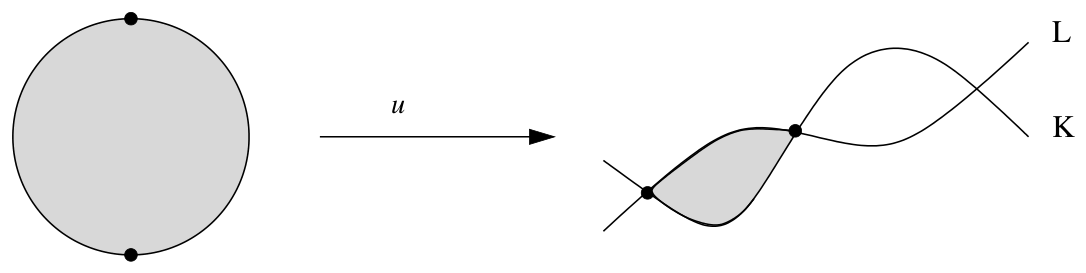
\includegraphics[width=0.55\textwidth]{fig01-floer-whitney.png}
  \caption{Floer 微分（即 $CF^*(L,K)$ 上的微分；原文 Figure~1，第 8 页）。\label{Fig:FloerWhitney}}
\end{figure}

设 $L \pitchfork L'$ 横截，并取 $H \equiv 0$。则方程 \eqref{eq:Floer} 就是通常的 Cauchy–Riemann 方程 $\cdbar_J(u) = 0$。存在共形等同 $\bR\times[0,1] \cong D^2 \backslash \{\pm i\}$，而 Floer 方程的解可延拓为闭圆盘上的连续映射，把 $\pm i$ 送到所选交点 $x_{\pm} \in L \cap L'$；在这个意义上，Floer 微分计数的是全纯圆盘，见图 \ref{Fig:FloerWhitney}。关键在于：(i) 对一般的数据，应当预期 \eqref{eq:Floer} 的解模空间是有限维光滑流形；(ii) 这些模空间具有几何上有意义的紧化。模空间的光滑性与有限维性是 Cauchy–Riemann 方程（带全实边界条件）椭圆性的推论；而面积一致有界的曲线空间之紧化的几何描述，则是 Deligne 与 Mumford 引入稳定曲线模空间那一思路的变体：边界层用带结点的 Riemann 曲面（圆盘与球面构成的树）来标号。

这是一个非平凡的定理（需要下面第 \ref{Sec:GeometricHyp} 节讨论的附加假设）：$d_J^2 = 0$，因此这确实定义了一个链复形。与 Morse 理论一样，$d_J^2=0$ 背后的机制是：\eqref{eq:Floer} 解的 1 维模空间具有紧化，其边界层标号出 $d_J^2$ 的各项贡献；而附加假设排除掉其他会打乱这种标号的不受欢迎的退化。
% [Tutor Note: $d_J^2=0$ 的证明不在正文，其要点是对（模去平移的）1 维解模空间做 Gromov 紧化：
%   边界层要么在角点处破裂、给出 $d_J\circ d_J$ 的各项，要么冒出圆盘泡/球面泡；只有排除后者，边界恒等式才恰好给出 $d_J^2=0$。
%   注意 $E(u) < \infty$ 这一条是紧化的定量前提，不能省略。]
在此前提下，相应的上同调 $HF^*(L,L')$ 就称为 Floer 上同调。一个“选择的同伦”论证说明它既不依赖 $J$ 的选取，也不依赖 $L$ 或 $L'$ 的 Hamilton 同痕。事实上，给定一族近复结构 $\{J_s\}$ 或一个在 $|s| \gg 0$ 时恒定的运动拉格朗日边界条件 $\{L_s\}$，人们考虑连续映射方程
\begin{equation} \label{Eqn:Continuation}
 \partial_s u + J_{s}(t,u) \big(\partial_tu - X_{s}(t,u)\big) = 0
\end{equation}  
其边界条件为 $\{L_s, L'\}$，解的数量给出相关 Floer 复形之间的链映射。把该映射与由逆同伦诱导的映射的复合形变回常值族，便可看出它在同调上诱导同构，而常值族诱导上同调上的恒等。

\begin{Example}
令 $X=T^*S^1$，考虑由 0-截面与一个同伦的圆给出的拉格朗日 $L, L'$，后者与该截面横截相交于两点 $a,b$。有两个跨接两圆的月牙形区域 $u,v$，由 Riemann 映射定理，它们共形地是全纯条带的像。复形 $CF(L, L') = \bK\langle a\rangle \oplus \bK\langle b\rangle$。取 $\bK = \bC$。按面积 $e^{-\int_u \omega}$ 对全纯条带 $u$ 加权计数，并计入全纯条带的定向，可得
\[
\partial(a) = (e^{-\omega(u)} - e^{-\omega(v)}) \, b, \qquad \partial(b) = 0.
\]
因此，除非 $\omega(u) = \omega(v)$，否则 $HF(L,L') =0$；确实，若面积不同，可以把 $L'$ Hamilton 同痕为一个与 $L$ 平行、与 $L$ 不交的平移。若两月牙形面积相等，则 $L'$ 是 $L$ 的 Hamilton 像，且 $HF(L,L')$ 的秩为 2。
\end{Example}

Floer 理论中的一篇典型论文总是先对环境几何给出一系列技术性假设。在第 \ref{Sec:GeometricHyp} 与第 \ref{Sec:AlgebraicHyp} 节中，我们汇集其中最常见的一些，指出它们各自在何处起作用，以及在其不成立或成立时人们能得到什么。

\subsection{定义的动机} 下面第一个动机在历史上是准确的，其余几个则提供了有用的背景。

\subsubsection{路径空间上的 Morse 理论} 设 $Q$ 是光滑有限维流形，$f: Q \rightarrow \bR$ 是一般函数（特别地，其临界点非退化），则 $f$ 的 Morse 复形 $C^*(f)$ 由 $f$ 的临界点生成，其微分计数梯度流线
\[
\gamma: \bR \rightarrow Q,  \quad \dot{\gamma}(t) = \nabla f_{\gamma(t)}
\]
其中梯度流是相对于 $Q$ 上某个辅助选取的 Riemann 度量而言的。有一个由 Novikov 给出的推广：把函数 $f$ 换成一个不一定恰当的一形式。Floer 复形正是该构造的形式类比：把 $Q$ 换成路径空间 $\mathcal{P}(L,L')$，把函数 $f$ 换成作用泛函（一形式）$\scrA$——它沿某条路径 $\gamma$ 的无穷小变分 $\xi$ 积分辛形式，即 $\xi \mapsto \int_0^1\omega(\xi, \dot{\gamma}) dt$，其中 $\xi$ 是沿 $\gamma$ 的向量场。$\scrA$ 的临界点是常值路径，也就是交点。固定 $(X,\omega)$ 上一个相容的近复结构 $J$，即 $J$ 驯服且 $\omega(J\cdot, J\cdot) = \omega(\cdot,\cdot)$。于是 $J$ 在路径空间上定义了一个 $L^2$-度量，而形式的梯度流方程恰是 $H=0$ 时的 Cauchy–Riemann 方程 \eqref{eq:Floer}。

\begin{Remark} \label{Rem:Filtration}
$HF^*(L,L')$ 的梯度流观点还揭示出额外的结构：若 $\scrA$ 是单值的，则复形 $CF^*(L,L')$ 自然被作用量（即泛函 $\scrA$ 的取值）滤过，而 Floer 微分保持该滤过。
% [Tutor Note: 这里“单值”是关键：作用量泛函一般只在覆叠空间上良定义，若辛形式在 $\pi_2(X,L)$ 上不零化，
%   则 $\scrA$ 多值，按作用量滤过只能在万有覆叠上谈；这正是后文要引入 Novikov 系数的原因之一。]
\end{Remark}

\subsubsection{几何相交数} 设 $\Sigma_g$ 是亏格为 $g$ 的定向曲面。对 $\Sigma$ 上（同伦非平凡的）曲线 $\alpha, \beta$，以 $\iota(\alpha,\beta) \in \bZ_{\geq 0}$ 记其几何相交数。一个微分同胚 $f$ 给出序列 $\iota(\alpha, f^n(\beta))$（$n\in \bN$），它只依赖 $f$ 的映射类 $[f] \in \pi_0\Diff(\Sigma)$。Nielsen–Thurston 分类可以用动力学的语言表述如下 \cite{FLP}：每个 $f$ 满足下列之一。

\begin{itemize}
\item $f$ 是可约的：若 $f$ 的某个幂保持一条简单闭曲线（同痕意义下）；
\item $f$ 是周期的：若对任意 $\alpha, \beta$，序列 $\{\iota(\alpha, f^n\beta)\}$ 关于 $n$ 是周期的；
\item $f$ 是伪 Anosov 的：若对任意 $\alpha,\beta$，序列 $\{\iota(\alpha, f^n\beta)\}$ 关于 $n$ 指数增长。
\end{itemize}

该分类应视为对曲面复杂度的归纳：可约情形表明 $f$（的某个幂）由某个更简单曲面的微分同胚诱导。在最有趣的伪 Anosov 情形，几何相交数增长率之对数与 $\alpha,\beta$ 无关，并且可由映射类 $f$ 在 Teichm\"uller 空间上作用的 Teichm\"uller 度量平移长度实现。$\Sigma$ 的任意微分同胚都同痕于一个保面积微分同胚。对不互相同伦（也不同伦平凡）的曲线 $\alpha, \beta$，有 $\iota(\alpha,\beta) = \mathrm{rk}\, HF(\alpha,\beta)$，所以 Thurston 分类同时也是用 Floer 上同调增长率对辛映射类作出的分类。在高维寻找类似物是一个长期挑战。

\subsubsection{手术理论} 高维流形的分类依赖 Whitney 技巧。考虑单连通定向流形 $M$ 中两个互补维数的可定向子流形 $K^k, N^{d-k} \subset M^d$，其中 $d>4$、$k>2$。设 $K,N$ 交于一对相交符号相反的点 $\{x,y\}$；在 $K$ 与 $N$ 中分别取连接 $x$ 与 $y$ 的弧，Whitney 技巧便让 $K$ 沿一张跨接这两条弧的圆盘滑动（该圆盘由 $M$ 的单连通性保证存在；由于 $d > 4$ 且 $k>2$，可假定它嵌入且内部与 $K,N$ 不交），从而降低子流形的几何相交数。Floer 上同调设想的是 Whitney 技巧的一个精细版本：只允许通过沿\emph{全纯} Whitney 圆盘滑动来消去拉格朗日子流形之间多余的相交。

Floer 上同调自身的手术论方面尚待发展，即：给定一对恰交于两点并界定唯一全纯圆盘的拉格朗日子流形 $L, L'$，何时能通过 Hamilton 同痕移动 $L$ 来消去这两个交点，目前未知。这是该理论最基本的空白之一。

\subsubsection{量子上同调} Floer 上同调是闭弦不变量（通过对有理曲线的计数来定义）的开弦类比（涉及带边界的亏格零 Riemann 曲面）。闭辛流形 $X$ 的量子上同调作为加群是 $H^*(X;\bK)$（$\bK$ 通常是 Novikov 域，参看 \eqref{Eqn:NovikovField}），但它带有乘法 $\ast$，该乘法用 3 点 Gromov–Witten 不变量决定的高阶贡献来形变经典的相交积。对光滑射影簇，它可以纯代数几何地定义，即通过稳定映射模栈上的相交理论。若 $\phi: X\rightarrow X$ 是辛同胚，则对角线 $\Delta_X$ 与 $\phi$ 的图像 $\Gamma_{\phi}$ 都是 $(X,\omega) \times (X,-\omega)$ 中的拉格朗日，于是定义\footnote{$HF^*(\phi)$ 有一个更初等、适用范围更广的直接构造；但为简洁起见，我们满足于通过拉格朗日 Floer 上同调来描述。} $CF^*(\phi) = CF^*(\Delta_X, \Gamma_{\phi})$。$CF^*(\phi)$ 的生成元由 $\phi$ 的不动点给出（假定这些不动点非退化）。为把两种讨论联系起来：有同构 $HF^*(\id) \cong QH^*(X)$。

量子上同调本身就是一个重要的不变量：它区分出若干有趣的辛流形集合（例如证明辛结构模微分同胚的模空间在 $K \times S^2$ 上有无穷多个分支，其中 $K \subset \bC\bP^3$ 是四次 $K3$ 曲面）；它在三维 flop 下不变；且与可积系统有深刻联系。若把 $QH^*(X) \cong HF^*(\Delta_X, \Delta_X)$ 视为一种影响深远的推广，那么一般拉格朗日对之间的 Floer 上同调的缺点在于：它很少能用代数几何方法计算——至少在镜像对称带来洞见之前如此。

\subsection{定义的技术细节：几何假设\label{Sec:GeometricHyp}}

低维拓扑与几何中的许多不变量都是通过计数某个椭圆偏微分方程的解来定义的。这样的定义预设：在好的情形下，模空间是紧的零维流形，因而计数才有意义。问题的核心于是归结为克服横截性（使解空间成为已知维数的流形）与紧性（使零维解空间成为有限集）这两方面的困难。

\subsubsection{横截性.} $X$ 上的驯服近复结构 $J$ 称为对某个特定的模问题\emph{正则}的（例如对映射 $u: \bP^1 \rightarrow X$，或对代表固定相对同调类、满足 $\cdbar_J(u) = 0$ 的圆盘 $u: (D^2,\partial D^2) \rightarrow (X,L)$），若 Cauchy–Riemann 方程或 Floer 方程的线性化 $D_u = D(\cdbar_J)_u$ 在每个解 $u$ 处都满射。在这种情形，Sard–Smale 隐函数定理表明解 $u$ 的模空间局部是光滑流形，其维数等于算子 $D_u$ 的指标。Sard–Smale 定理涉及 Banach 流形之间的映射，因此有一个常规的麻烦：应先把 $\cdbar$-算子延拓为 Banach 丛 $\cdbar_J: L^{k,p}(\Sigma, X) \rightarrow L^{k-1,p}(\mathcal{E})$ 的一个截面（其中 $\mathcal{E}_u = \Omega^{0,1}(u^*TX)$），定义在 $L^{k,p}$ 映射空间上（若 $kp>2$ 则映射连续，逐点边界条件才有意义），从而对正则的 $J$ 得到光滑的解模空间——它\emph{先验地}由低正则性的映射组成；然后再用“自举（bootstrapping）”推出方程的任一 $L^{k,p}$-解其实都是光滑映射。
% [Tutor Note: Sard–Smale 只适用于可分 Banach 流形之间的 Fredholm 截面，所以必须先做 $L^{k,p}$ 完备化；
%   把“解”直接当成 $C^\infty$ 映射来谈横截性是常见的形式错误。椭圆正则性负责把 $L^{k,p}$ 解提升回光滑解。]

达到“你想要的那么多横截性”存在内在障碍。例如设 $X$ 是闭辛 6-流形且 $c_1(X) =0$。对任意 $A \in H_2(X;\bZ)$，类 $A$ 中无参数有理曲线的虚拟维数为 $0$。然而，若 $u: \bP^1 \rightarrow X$ 代表类 $A$，则类 $kA$ 可由映射 $\bP^1 \stackrel{k:1}{\longrightarrow} \bP^1 \stackrel{u}{\longrightarrow} X$ 代表，于是类 $kA$ 中曲线的模空间至少和 $\bP^1$ 到自身的 $k$ 次覆盖的 Hurwitz 空间一样大，不可能维数为零。这说明：若不扰动 Floer 方程或 Cauchy–Riemann 方程本身以破坏覆盖的对称性（例如让近复结构 $J$ 依赖曲线的定义域上的点，从而不具任何有限对称性），就不能指望在多重覆盖曲线上达到横截性。对有理曲线，一般选取的 $J$ 对单重（非多重覆盖）曲线是正则的。对圆盘，若视其为条带 $D^2 \backslash \{\pm 1\}$ 上在边界穿孔处光滑延拓的映射，则一族一般的复结构 $\{J_t\}_{t\in[0,1]}$ 对具有内射点 $x$（即满足 $u^{-1}(u(x)) = \{x\}$ 的点）的解仍是正则的。

\begin{Example} \label{Ex:TransversalityFiniteGroup} 还有与多重覆盖无关的横截性问题。设 $X$ 带有一个辛对合 $\iota$，其不动点集为 $X^{\iota}$，并设有 $\iota$-不变的拉格朗日 $L_i$，满足 $L_i^{\iota} = L_i \cap X^{\iota}$ 是 $X^{\iota}$ 中的拉格朗日。若对 $x,y \in L_1^{\iota} \cap L_2^{\iota}$，含于 $X^{\iota}$ 内的 Floer 轨道 $u$ 所在模空间的虚拟维数大于 $u$ 在 $X$ 中相应的虚拟维数，则不能同时要求该曲线在两个空间中都正则：正则 $J$ 的稠密集可能与 $\iota$-不变 $J$ 的无限余维轨迹不相交。（若不动点集中没有轨道，则\emph{可以}实现等变横截性 \cite{Khovanov-Seidel}。）
% [Tutor Note: 等变横截性失败的机制值得记住：正则 $J$ 是稠开集，而 $\iota$-不变 $J$ 是无限余维的闭子集，二者可能不交。
%   因此不能“先取一般 $J$ 再对称化”；正确做法是在等变范畴内单独做横截性论证（如固定轨迹内无轨道时）。]
\end{Example}

\subsubsection{通过冒泡的紧性.} 解模空间即使正则，通常也不紧。Gromov 紧性 \cite{Gromov} 给出一个紧化，其中包含带结点的曲线（球面与圆盘构成的树）。一个要点是：虽然 Floer 方程是 Cauchy–Riemann 方程的形变版本，泡却来自重新尺度化过程，这意味着它们满足未形变的方程 $\overline{\partial}_J(u) = 0$。因此，一般不能指望通过一般地选取非齐次项或依赖定义域的近复结构来克服多重覆盖泡带来的横截性问题。通常，全纯曲线紧化空间的边界层维数可能远大于人们想要紧化的开层维数。对此没有容易的一般性解决办法（已有的解法 \cite{FO3:technical, HWZ} 是在映射的 Banach 空间内扰动解模空间，而不是扰动方程或其他几何数据本身，统称为\emph{虚拟扰动理论}）。

具体地说，要定义 Floer 上同调，需要知道 Floer 复形中 $d^2 = 0$。与 Morse 理论一样，这一关系的证明来自研究（模去平移的）1 维解模空间的边界。除了对 $d^2$ 有贡献的边界层之外，还有一种有问题的破裂：一个以 $L$ 或 $L'$ 为边界的全纯圆盘从中冒出，见图 \ref{Fig:Bubble}。（圆盘的边界值被一个常值映射送到拉格朗日上、从而给出 $X$ 中经过 $L$ 的有理曲线这一退化情形，同样有问题。）

\begin{figure}[ht]
  \centering
  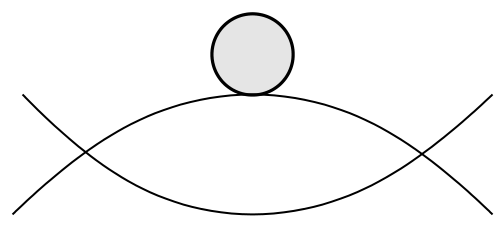
\includegraphics[width=0.4\textwidth]{fig02-disc-bubble.png}
  \caption{全纯圆盘泡会阻碍 Floer 复形中的 $d^2 = 0$（原文 Figure~2，第 12 页）。\label{Fig:Bubble}}
\end{figure}

有三种基本路线可以回避圆盘冒泡带来的问题。
% [Tutor Note: 三条路线不要混为一谈：(i) 非球性/恰当性——面积上根本不容许泡存在；
%   (ii) 单调性——允许泡，但按虚拟维数它扫出的链在 $L$ 中是边界，故对 $d^2$ 无贡献；
%   (iii) 障碍理论——允许泡贡献，用界定上链把这些边界“配平”。恰当性蕴含非球性，但反之不然。]

\subsubsection{先验地排除泡：非球性或恰当性.\label{Sec:exact}} 这里要求对所考虑的一切拉格朗日都有 $\langle \omega, \pi_2(X,L)\rangle = 0$（这特别蕴含 $X$ 中没有辛 2-球面）。由于泡是全纯的，若非常值，其面积必严格为正，这由基本恒等式
\[
\int_C u^*\omega \ = \ \int_C \| du\|_J^2
\] 
对带拉格朗日边界、$J$ 与 $\omega$ 相容的 $J$-全纯曲线 $u: C \rightarrow X$ 成立。这是本学科最早几篇论文（尤其是 Floer 本人的工作）所采用的设定。

对非紧辛流形 $X$，若辛形式 $\omega = d\theta$ 整体恰当，且拉格朗日 $L\subset X$ 是恰当的（即 $\theta|_L = df$ 在 $H^1(L)$ 中为零），则由 Stokes 定理立即排除泡。（然而 $\omega^n > 0$ 表明 $\omega$ 的恰当性与 $X$ 为闭流形不相容。）$X$ 的非紧性引入模空间失去紧性的另一个可能来源：解可能逃逸到无穷远；这由另一套机制控制，通常是某种极值原理的变体，它要求对无穷远处的几何加以控制。Stein 流形 $X$（特别是仿射簇）在无穷远处以接触锥为模型，即紧集之外它们辛同胚于 $(Y\times \bR_+, d(e^t\alpha))$ 的某个子集，其中 $(Y,\alpha)$ 是接触的、$t\in\bR_+$。对全纯曲线 $u: \Sigma \rightarrow X$，（部分定义的）函数 $t\circ u$ 是次调和的，$\Delta(t\circ u) \geq 0$，这意味着该函数没有内部最大值。由此推出：边界包含在内部 $X \backslash (X \cap Y\times\bR_+)$ 中的全纯曲线完全含于内部，因此 Stein 流形在前文所述意义下在无穷远处凸。

一个可追溯到 Floer 的论证，把 $L, \phi_H^t(L)$（其中 $\phi_H^t$ 是 $L$ 上某个 Morse 函数 $H$ 的小时间流，$J$ 是仔细选取的时间依赖近复结构）之间的、保持在 $L$ 附近的全纯条带，与 $H$ 的梯度流线等同起来。因此作为向量空间可以认同 $CF^*(L,L) = C^*_{Morse}(L)$。在不存在以 $L$ 为边界的全纯圆盘时，紧性论证表明没有其他能对 Floer 微分有贡献的全纯条带，从而：

\begin{Theorem}[Floer] \label{Lem:Floer}
若 $\langle \omega, \pi_2(X,L) \rangle = 0$，则 $HF^*(L,L) \cong H^*(L)$。
\end{Theorem}

这恢复了 Gromov 的定理 \cite{Gromov}：$\bC^n$ 不含闭的恰当拉格朗日——因为这样的 $L$ 可被移开，从而 $HF(L,L)=0$。（恰当拉格朗日 $L_t$ 的任何同痕 $\{L_t\} \subset X$ 都由 $X$ 的 Hamilton 流诱导；特别地，恰当同痕不改变 Floer 上同调。）

\subsubsection{因维数理由排除泡：单调性.\label{Sec:Monotone}} 若可能的圆盘泡与球面泡所扫出的 $X$ 的子集具有足够高的（余）维数，则对 Floer 方程中数据的\emph{一般}选取（近复结构、Hamilton 项），1 维模空间中出现的全纯条带的边界值永远不会与泡相交。这一解决办法的典型情形是 $X$ 与 $L$ 都\emph{单调}，即 Maslov 指标 $\mu_L$ 与面积同态在 $\pi_2(X,L)$ 上正比例；特别地，$\omega_X$ 与 $c_1(X)$ 在 $\pi_2(X)$ 上正比例，这是代数几何中 Fano 条件的辛类比。$\bP^n$ 中总次数 $\leq n$ 足够低的超曲面或完全交是单调的。单调辛流形的极小 Chern 数 $N_{min}(X)>0$ 由等式 $\{\langle c_1(X), \pi_2(X)\rangle\} = N_{min}(X)\bZ$ 定义。类似地，单调拉格朗日 $L\subset X$ 有极小 Maslov 数 $N_{min}(L)>0$。由于在 $H^2(X,L)\rightarrow H^2(X)$ 之下 $\mu_L \mapsto 2c_1(X)$，当 $\pi_1(L)=0$ 时 $N_{min}(L) = 2N_{min}(X)$。
% [Tutor Note: $\mu_L \mapsto 2c_1(X)$ 中的因子 2 来自 Maslov 指标与 Chern 数的换算（圆盘边界绕行时切空间转两圈）。
%   由此 $N_{min}(L)=2N_{min}(X)$（当 $\pi_1(L)=0$）；核对 $\frak{m}_0$ 与单调性假设时，此处最容易差一个因子 2。]

先设 $X$ 单调且 $N_{min}(X) \geq 2$，而 $K, L\subset X$ 是单调拉格朗日，各自 $N_{min}\geq 4$。图 \ref{Fig:Bubble} 所描绘的构型，形式上是一个纤维积 $\scrM_{bubble} \times_L \scrM_{Floer}$：Floer 条带空间与圆盘泡空间的纤维积，沿（假定光滑且横截的）到 $L$ 的赋值映射取。某个类 $\beta$ 中 $L$ 上无参数圆盘的模空间的虚拟维数为 $n+\mu_L(\beta)-3 \geq n+1$，故赋值后在 $L$ 上作为链是平凡的，即它们是 $C^*_{sing}(L)$ 中的边界。这意味着在代数上，计算 $CF^*(K,L)$ 中的 $d^2$ 时不会出现带圆盘泡的退化。

在极小 Maslov 指标为 2 的单调拉格朗日这一特殊情形，有一点细微却重要的差别：Maslov 2 圆盘的模空间是 $(n-1)$ 维的，在边界标记点处赋值后，类 $\beta$ 的圆盘以某个重数 $n_{\beta}$ 扫出 $L$。这引出一个特殊的“障碍项”
\[
\frak{m}_0(L) = \sum_{\beta} n_{\beta} q^{\langle \omega, \beta\rangle} \in \bC[\![q]\!].
\] 对满足 $\frak{m}_0(L) = \frak{m}_0(L')$ 的拉格朗日对 $L, L'$，仍可定义 Floer 上同调，因为此时相关的额外边界可以互相抵消；但对 $\frak{m}_0$ 值不同的单调拉格朗日，Floer 复形中\emph{不}成立 $d^2=0$。

\begin{Example} \label{Ex:CY} 若 $X$ 是 Calabi–Yau 曲面，则 Maslov 零的拉格朗日的圆盘泡虚拟维数为负：$n+\mu-3 = -1$，故对一般的 $J$ 没有泡，可以把 $CF^*(L,L)$ 定义为上链复形。然而，在拉格朗日的一参数族中可能出现孤立的圆盘泡，这意味着所得的 Floer 上同调\emph{先验地}不清楚是否 Hamilton 不变：连续映射方程 \eqref{Eqn:Continuation} 可能因冒泡而不是链映射。参看 \cite[Section 8]{Seidel:HMSquartic}。
% [Tutor Note: 虚拟维数为负只保证“一般 $J$ 下没有泡”，不保证一族 $J_t$ 或一族 $L_t$ 中没有孤立泡；
%   这正是“$HF$ 定义出来了、却未必 Hamilton 不变”的典型陷阱，需要额外论证连续映射是链映射。]
\end{Example}

\subsubsection{消去泡：障碍理论} 若圆盘泡出现，它们会给 1 维模空间添上多余的边界，使 $d^2=0$ 不成立。若能“手工”抵消这些多余边界，便可挽救局面：在图 \ref{Fig:Bubble} 中，赋值像 $ev(\scrM_{bubble}) \in C^*_{sing}(L)$ 可能是边界，尽管并非因维数理由而平凡地是边界。这正是 Floer 上同调的\emph{障碍理论}的起源。它并不总是适用（圆盘泡边界扫出的 $L$ 中轨迹可能不是零调的），适用时又依赖于界定上链的额外选取（这使 Hamilton 不变性变得复杂，参看例 \ref{Ex:CY}），但它提供了 Floer 理论迄今得以发展的最一般框架，尤其是 \cite{FO3, FO3:technical}。这一策略奏效的情形类足够宽广，比起其他几种是相当大的进展，但这项工作的细节——一般要依赖虚拟扰动理论——颇为可畏。

为照顾一般情形，Floer 上同调有良好定义的拉格朗日被称为\emph{无障碍的}。

\subsection{定义的技术细节：代数假设\label{Sec:AlgebraicHyp}} 即使已经决定了允许哪一类拉格朗日子流形，它们所携带的附加结构仍有种种变化（这些结构的存在性可能施加进一步的限制）。

\subsubsection{系数环的选取.\label{Sec:Novikov}}

Gromov 紧性在有统一面积界时可控制全纯曲线序列的极限；但——正如 Novikov 的圆周值 Morse 理论——一个问题中仍可能遇到无穷多个模空间（此处是一对固定交点之间的连接条带）。若出现无穷多个模空间，为使和式 \eqref{Eqn:FloerDifferential} 有意义，就需要追踪同伦类。于是，$HF^*$ 最一般适用的定义要在 Novikov 域
\begin{equation} \label{Eqn:NovikovField}
\Lambda \ = \ \left\{ \sum a_i q^{\lambda_i} \ | \ a_i \in \bK, \lambda_i \in \bR, \lambda_i \rightarrow \infty \right\}
\end{equation}
上工作，其底层系数域为 $\bK$（若 $\bK$ 代数闭，则 $\Lambda$ 也代数闭）。然后定义 Floer 微分 \eqref{Eqn:FloerDifferential} 为
\begin{equation} \label{Eqn:FloerDifferential-Novikov}
d_J(x_+) = \sum_{\beta, x_-} n^{\beta}_{x_+, x_-} q^{\langle \omega, \beta\rangle} x_-
\end{equation}
其中 $\beta$ 是连接双边形的同伦类。有一个子环 $\Lambda_+ \subset \Lambda$，由最低 $q$ 幂次 $\geq 0$ 的幂级数组成。Floer 上同调只有在 Novikov 域上工作时才对 Hamilton 同痕不变；尽管如此，它在 $\Lambda_+$ 上仍承载非平凡信息。有限生成 $\Lambda_+$-模的分类定理表明
\[
HF(L,L') \cong \Lambda_+^r \, \bigoplus \ \oplus_{i=1}^n \Lambda_+ / \langle q^{k_i} \rangle
\]
挠部分在过渡到 $\Lambda$ 时显然消失，而自由加项保留下来；另一方面，显式的 Hamilton 同痕只能把系数 $k_i$ 改变不超过该同痕的 Hofer 范数——这是转到 Novikov 域上工作时丢失的信息。这一点在圆 $S^1 \subset \bC$ 这一最平凡的情形就已显现。该圆是 Hamilton 可移开的，故在 $\Lambda$ 上其自 Floer 上同调消失；而在环 $\Lambda_+$ 上自 Floer 上同调是挠群 $\Lambda_+ / \langle q^A \rangle$，其中 $A$ 是该圆所围的面积。于是，$\Lambda_+$ 上的 Floer 上同调记住了（在此情形下是初等的）事实：任何移开它的 Hamilton 量至少要用能量 $A$。
% [Tutor Note: $\Lambda$ 与 $\Lambda_+$ 的取舍是实用分水岭：只有 $\Lambda$ 上才有 Hamilton 同痕不变性；
%   而 $\Lambda_+$ 保留了 Hofer 范数能探测的能量下界（圆 $S^1\subset\bC$ 是最清楚的例子）。
%   另注意 $\Lambda$ 的指数满足 $\lambda_i \to +\infty$（形式幂级数），方向与通常 Laurent 级数相反。]

\begin{Example}
若 $L, L'$ 恰当，$\theta|_L = df$、$\theta|_{L'} = df'$，则交点 $x,y \in L\pitchfork L'$ 之间任一连通全纯条带的面积由 $f(x)-f'(y)$ 给出。统一的面积界与 Gromov 紧性蕴含只有有限多个同伦类 $\beta$ 能由全纯条带实现，因此和式 \eqref{Eqn:FloerDifferential} 是有限的。
\end{Example}

\subsubsection{Spin 结构与扭曲理论}

至此我们尚未提及域 $\bK$ 的特征。若它不等于 2，则 \eqref{Eqn:FloerDifferential} 或 \eqref{Eqn:FloerDifferential-Novikov} 中的计数必须是 0 维模空间的\emph{带符号}计数，因此这些模空间应当可定向。一个基本事实 \cite{deSilva,FO3} 是：$L$ 上 $Spin$ 结构的一个选取\footnote{用 $Pin$ 结构也够，但我们坚持用 $Spin$。}诱导出某个类 $\beta$ 中 $L$ 上全纯圆盘模空间 $\scrM(\beta)$ 的一个定向；环路 $\gamma: S^1 \rightarrow \scrM(\beta)$ 通过取边界值诱导映射 $\Gamma_{\gamma}: T^2 \rightarrow L$，且 $\langle w_1(\scrM(\beta)), \gamma\rangle = \langle w_2(L), \Gamma_{\gamma}\rangle$。同理，若 $L$ 不是 $Spin$ 的，就不能指望圆盘或 Floer 轨道的模空间可定向，此时应在特征 2 下工作。

拉格朗日上 $Spin$ 结构的存在意味着模空间具有定向。然而这些定向仍非典范的：人们可以用任一全纯圆盘与 $X$ 中某个与拉格朗日不交的余维 2 闭链的相交数，来扭转该圆盘计入 Floer 微分的符号；这种扭转与曲线的破裂以及由此定义 Floer 上同调（及其上以后会遇到的各种运算）的模空间紧化相容。结论是：实际上对任意“背景”类 $\beta \in H^2(X;\bZ_2)$ 的选择，都有一个版本的 Floer 上同调 $HF^*(L,L';\beta)$，其中拉格朗日应在“相对 spin”的意义下满足 $w_2(L) + \beta|_L = 0$。

\subsubsection{分次} 与经典代数拓扑的链复形不同，Floer 复形一般不是 $\bZ$-分次的。至少当拉格朗日子流形 $L, L'$ 定向时，横截交点有正负之分，这在复形上诱导一个 $\bZ_2$-分次（若拉格朗日可定向但未定向，这仍作为相对 $\bZ_2$-分次保留下来）。这可以细化为 $\bZ/N$ 分次，其中 $N$ 是拉格朗日的极小 Maslov 数。特别地，若 $L$ 与 $L'$ 的 Maslov 类为零（这尤其要求 $2c_1(X)=0$），则 Floer 复形可以 $\bZ$-分次。
% [Tutor Note: 分次有三个层次，切勿混用：$\bZ_2$（来自定向）$\subseteq$ $\bZ/N$（$N$ 为极小 Maslov 数）$\subseteq$ $\bZ$（Maslov 类为零，需 $2c_1(X)=0$）。
%   同一公式在不同分次下的次数可能相差 $N$ 的倍数，引用时务必先确认用的是哪一种。]

\subsection{应用 I}\label{Sec:Appl1} 正如开头所指出的，若 $HF^*(L,L') \neq 0$，则 $L$ 与 $L'$ 不能通过 Hamilton 同痕彼此移开。最早的应用中有若干是这一主题的变体：下面几例取自 \cite{Lalonde-Sikorav, FSS2, Polterovich}。

\subsubsection{近邻拉格朗日子流形} 若 $L\subset M$ 是拉格朗日，则 $M$ 局部以带标准辛结构的余切丛 $(T^*L, d\theta)$ 为模型。这意味着拉格朗日嵌入的分类问题至少和余切丛中拉格朗日的局部分类问题一样复杂。Arnol'd 猜想（参看问题 \ref{Q:Arnold}）：若 $K\subset T^*L$ 是闭的\emph{恰当}拉格朗日，则它应当与零截面 Hamilton 同痕。特别地
\begin{itemize}
\item  $HF^*(K,L) \cong HF^*(L,L) = H^*(L)$ 应当非零，从而 $K$ 应当与零截面 $L\subset T^*L$ 相交；
\item  $K \subset T^*L \rightarrow L$ 应当是度一映射，因而满射。
\end{itemize}
% [Tutor Note: 证明的骨架是“按面积滤过 + 谱序列”：先让 $c\to\infty$ 把 $cK$ 压成若干条余切纤维的并，
%   再借注 \ref{Rem:Filtration} 的作用量滤过把纤维的 Floer 群拼回 $K$ 的 Floer 群。这里只能得到“相交非空”与“投影满”，
%   度 $=1$ 需要更精细的论证（见 §4.5）。]

$T^*L$ 有一个重新尺度化作用，把纤维乘以常数 $c$；重尺度化后的子流形 $cK$ 都恰当，因而互相 Hamilton 同痕。令 $c\rightarrow \infty$，则子流形 $cK$ 逼近纤维之并 $\bigcup_{x \in K \cap L} T_x^*L$。在这幅示意图像里，$L$ 与 $cK$ 之间的全纯条带要么保持靠近单条余切纤维，要么扫出余切丛的一大片区域。按面积对全纯圆盘过滤，便得到谱序列，参看注 \ref{Rem:Filtration}：
\begin{equation} \label{Eqn:FibresShouldGenerate}
\bigoplus_{x\in K\cap L} \, HF^*(K, T_x^*L) \ \Longrightarrow \ HF^*(K,cK) = H^*(K)
\end{equation}
（最后的等式由定理 \ref{Lem:Floer} 给出。）于是可断定 $L\cap K \neq \emptyset$，并且对 $x\in L\cap K$ 有 $HF^*(K, T_x^*L) \neq 0$。然而由适当的连续论证，群 $HF^*(K, T_x^*L)$ 与 $x$ 的选取无关，这给出第二个断言的第二半：投影 $K \rightarrow L$ 是满射。就目前而言，这一论证\emph{不}足以断定投影映射的度为 1；我们稍后会在第 \ref{Sec:NearbyLag} 节推出这一点。

\subsubsection{映射类群} 回忆第 \ref{Sec:AlgFamily} 节中的二次映射 $\pi: \bC^{n+1} \rightarrow \bC$，$(z_1,\ldots,z_{n+1}) \mapsto \sum z_j^2$。一般纤维 $\pi^{-1}(1) \subset (\bC^{n+1}, \omega_{\st})$ 辛同胚于 $(T^*S^n, d\theta)$。该纤维化的单值（monodromy）同痕于一个紧支辛同胚，即\emph{Dehn 扭转} $\tau \in \pi_0\Symp_{ct}(T^*S^n)$；它也可以更直接地定义如下。$S^n$ 上圆度量的测地流是周期的，周期为 $\pi$。取 Hamilton 函数 $H:T^*S^n \rightarrow \bR$，它是 $r=|p|$（纤维坐标的范数）的函数，在 $|p| \ll 1$ 时为零，在 $|p| \geq 1$ 时斜率为 $\pi$。于是定义 $\tau$ 为 $T^*S^n$ 的（按构造是紧支的）辛同胚，它由复合（对径映射）$\circ \phi_H^1$ 给出。

我们断言，对 $n\geq 1$，$\tau$ 是 $\pi_0\Symp_{ct}(T^*S^n)$ 中的无限阶元素。（$n$ 为奇数时这是初等的，由同调考虑可得；但在偶数维，该映射在光滑映射类群中是有限阶的。）

考虑 Floer 上同调 $HF^*(\tau^m (T_x^*), T_y^*)$，其中 $x, y$ 互异但不互为对径。虽然这些拉格朗日非紧，但交点落在一个紧集中，且拉格朗日恰当、在无穷远处以 Legendrian 锥为模型，这意味着 $HF$ 可以毫无问题地定义（另一种做法是把相关的两条余切纤维封顶，得到含 $A_3$-链的拉格朗日球面的空间；与第 \ref{Sec:MCGIII} 节比较）。此外，由于 $c_1(T^*S^n) = 0$ 且拉格朗日的 Maslov 类平凡，$HF$ 还是 $\bZ$-分次的。Floer 复形的生成元对应绕相应大圆至多 $m$ 圈的测地线。Floer 复形中的 $\bZ$-分次重现了测地线作为环路空间上能量泛函临界点的 Morse 分次（由 Jacobi 场的数目决定），并且可以算出 \cite{FrauSchlenk}：$CF^*(\tau^m (T_x^*), T_y^*)$ 集中在次数
\[
(2n-2) \{0,1,...,(m-1)\}, \ \mathrm{and} \ (3n-3)\{0,1,...,(m-1)\}.
\]
若 $n \geq 3$，这些群从不出现在相邻的次数，Floer 微分消失，而 Floer 群的秩随 $m$ 增长。该结果在 $n=2$ 时也成立，但需要额外一步：例如可以对一个辛对合做等变处理，化归到 $T^*S^1$ 这一较易情形（在该不动点集中，由同伦理由没有 Floer 微分，即可以实现等变横截性，参看例 \ref{Ex:TransversalityFiniteGroup}）。

%%%%%%%%%%%%%%%%%%%%%%%%%%%%%%%%%%%%%%%%%%%%%%%%%%%%%%%%%%%%%%%%%%%%%%%%%%%%%%%
% 说明：本文件只覆盖 §3.1–§3.5（源码 508–727 行），因此只含 Figure 1 与 Figure 2 两幅图。
% §3.6 起的三幅图（无编号示意图、Figure 3、Figure 4）由 s03b-floer.tex 负责，此处不插入。
%%%%%%%%%%%%%%%%%%%%%%%%%%%%%%%%%%%%%%%%%%%%%%%%%%%%%%%%%%%%%%%%%%%%%%%%%%%%%%%



%%%%%%%%%%%%%%%%%%%%%%%%%%%%%%%%%%%%%%%%%%%%%%%%%%%%%%%%%%%%%%%%%%%%%%%%%%%%%%%
%%  [Inlined] s03b-floer
%%%%%%%%%%%%%%%%%%%%%%%%%%%%%%%%%%%%%%%%%%%%%%%%%%%%%%%%%%%%%%%%%%%%%%%%%%%%%%%
%%%%%%%%%%%%%%%%%%%%%%%%%%%%%%%%%%%%%%%%%%%%%%%%%%%%%%%%%%%%%%%%%%%%%%%%%%%%%%%
%  s03b-floer.tex —— 第 3 节后半（§3.6–§3.9，对应原文 pp.17–24）
%  说明：本文件续接 s03a-floer.tex，不再重复 \section 与 keypoints。
%  原文行区间：Prolegomenon_utf8.tex 第 728–962 行。
%%%%%%%%%%%%%%%%%%%%%%%%%%%%%%%%%%%%%%%%%%%%%%%%%%%%%%%%%%%%%%%%%%%%%%%%%%%%%%%

\subsection{代数结构}

Floer 上链群拥有丰富的附加结构；我们先从那些确实会下降到上同调中成为结构的（链层次）构造讲起。

\subsubsection{乘积结构}

给定三个拉格朗日子流形 $L,M,N \subset X$，存在一个零次乘积
\[
\mu^2: HF^*(M,N) \otimes HF^*(L,M) \longrightarrow HF^*(L,N)
\]
它由下图示意给出的全纯三角乘积所定义。
\begin{center}
  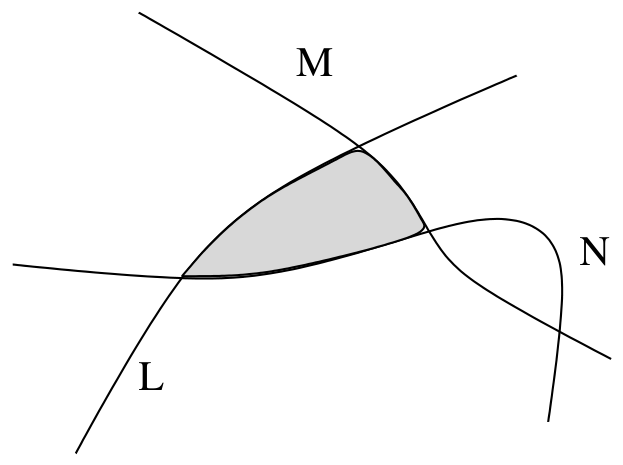
\includegraphics[width=0.4\textwidth]{fig03-floer-product.png}
\end{center}
% [Tutor Note: $\mu^2$ 的两个输入次序极易写反。本文的约定是 $\mu^2(x,y)$ 中 $x\in HF^*(M,N)$
%   为“较晚”的态射、$y\in HF^*(L,M)$ 为“较早”的态射，故合成顺序是“先 $y$ 后 $x$”；
%   而 $H(\scrA)$ 中的结合合成带着分次符号 $[a]\cdot[b]=(-1)^{|b|}[\mu^2(a,b)]$。
%   本节的三角乘积与 §4.1 的 $A_\infty$ 约定必须一致，核对时以 $(-1)^{|a|}$ 是作用在
%   第一个变元还是第二个变元上为第一要务（链层次关系 $d\mu^2(x,y)=\mu^2(dx,y)\pm\mu^2(x,dy)$
%   的符号随此约定联动）。]

图中表明：给定 $L\cap M$ 与 $M \cap N$ 中的输入交点（假定横截），某个给定输出点（位于 $L\cap N$）的系数由图中所示的一族三角形的计数给出；这里照例有若干保留条件：只计数零维模空间的元素，需在适当的几何假设下保证紧性，并且在原则上可以有无穷多个不同模空间作出贡献时要取 Novikov 系数。

\begin{figure}[ht]
  \centering
  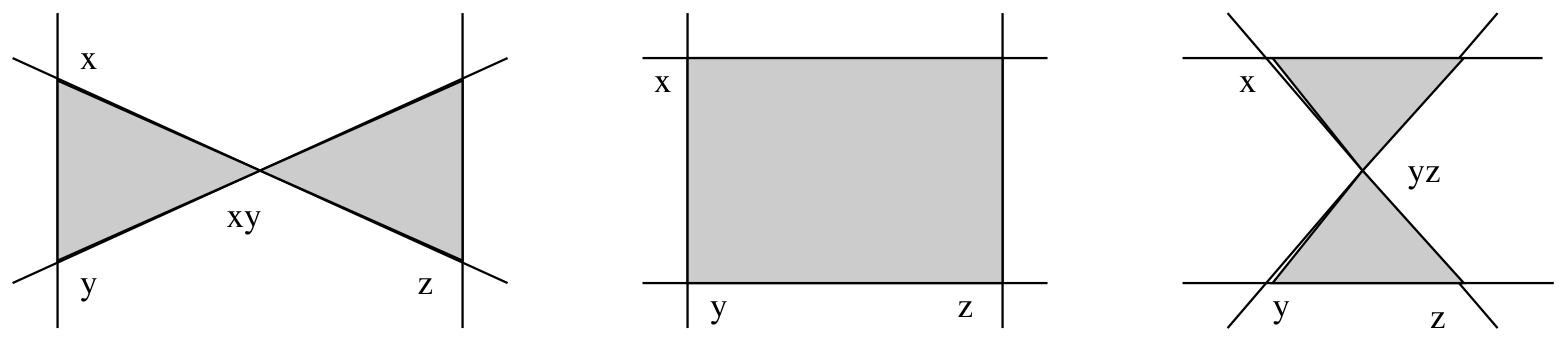
\includegraphics[width=0.78\textwidth]{fig04-triangle-assoc.png}
  \caption{三角乘积在上同调上满足结合律（原文 Figure~3，第 17 页）。\label{Fig:BrokenTriangles}}
\end{figure}

链层次运算之所以能下降到上同调，反映的是如下事实：模去冒泡之后，此类三角形的一维模空间的边界由“在角点处断开”的破裂构型所给出的层组成，而这些层在某个固定输出交点处的系数正是 $\mu^2(d(x),y)$、$\mu^2(x,d(y))$ 与 $d\mu^2(x,y)$ 的系数，其中 $d$ 是 Floer 微分。类似地，四边形的 1 维模空间可以如图 \ref{Fig:BrokenTriangles} 所示那样破裂，这表明三角乘积在上同调上结合：若所有输入都是 Floer 闭链，即 $d(\cdot) = 0$，则只有那两个“拼接三角形”的图形给出该一维模空间边界上非平凡的层，而它们分别对应 $\mu^2(x,\mu^2(y,z))$ 与 $\mu^2(\mu^2(x,y),z)$ 中右上交点的系数。

由此可知，对单个拉格朗日子流形 $L$，$HF^*(L,L)$ 自然地构成一个环，而且还是有单位元的环。环 $HF^*(L,L)$ 具有 Poincaré 对偶，它来自把全纯条带两侧的边界条件互换。事实上，存在迹 $\tr: HF^{n}(L,L) \rightarrow \bK$，它与三角乘积一起给出非退化配对
\[
HF^*(K,L) \otimes HF^{n-*}(L,K) \stackrel{\tr}{\longrightarrow} \bK.
\]
% [Tutor Note: 这里的 Poincaré 对偶就是“交换条带两端的边界条件”：$\tr$ 只在最高次
%   $HF^{n}(L,L)$ 上取值，配对 $HF^*(K,L)\otimes HF^{n-*}(L,K)\to\bK$ 把 $(x,y)$ 送到
%   $\tr(\mu^2(x,y))$。注意次数是 $n-*$ 而不是 $n+*$，且配对两侧 $K,L$ 的次序互换；
%   若定向或分次约定取反，$\tr$ 可能整体差一个 $(-1)^{n(n+1)/2}$，这与 §1 中相交数
%   公式的符号因子是同一个来源。]

下面的命题本质上属于 Oh \cite{Oh:Thomas}（与环结构的相容性在 \cite{Buhovski:ring} 中被明确写出），另见 \cite{Albers,BiranCornea}。它给出了本学科中的一个关键计算工具。

\begin{Proposition}\label{Lem:Oh}
存在谱序列 $H^*(L;\Lambda) \Rightarrow HF^*(L,L)$，它与普通上同调与 Floer 上同调中的环结构相容。
\end{Proposition}

\begin{proof}[证明概要]
固定 Morse 函数 $f: L \rightarrow \bR$。如定理 \ref{Lem:Floer} 中那样，对适当的 $J$，Morse 流线可用来定义 Floer 轨道。该谱序列来自按作用量对 Floer 微分作过滤，使得所有低能量解都来自 Morse 轨道。在作用量与指标相关的单调情形，该谱序列来自把 Floer 微分写成和式 $\partial_0 + \partial_1 + \cdots + \partial_k$，其中 $\partial_0$ 是 $C^*_{Morse}(L)$ 中的 Morse 微分，而 $\partial_i$ 的次数为 $1-iN_L$，$N_L$ 是 $L$ 的极小 Maslov 数。更形象地说，Floer 上同调有一个 Morse–Bott（或“珠串”）模型 \cite{BiranCornea}，其中 Floer 微分计数被 $L$ 上的全纯圆盘打断的 $f$ 的梯度线，参见图 \ref{Fig:PearlyGradient}，而 $\partial_i$ 所计数的构型中圆盘的总 Maslov 指标为 $iN_L$。Morse 乘积计数流线构成的 $Y$-树，这可以推广到珠串构成的 $Y$-形图，由此给出谱序列与环结构的相容性。
\end{proof}
% [Tutor Note: 谱序列的过滤是“按作用量”而不是“按次数”：低能量解只剩 Morse 流线，
%   于是 $E_1$ 页为 $H^*(L;\Lambda)$，微分逐级修正全纯圆盘的贡献。单调情形下
%   能量与指标相关，才可以把 $\partial$ 按圆盘总 Maslov 指标 $iN_L$ 拆成
%   $\partial_0+\partial_1+\cdots$，且 $\deg\partial_i=1-iN_L$；若能量—指标不相关，
%   “按作用量过滤”给出的只是收敛的滤过而非按次数的直和分解。收敛方向是
%   $H^*(L)\Rightarrow HF^*(L,L)$，核对时勿写反。]

\begin{figure}[ht]
  \centering
  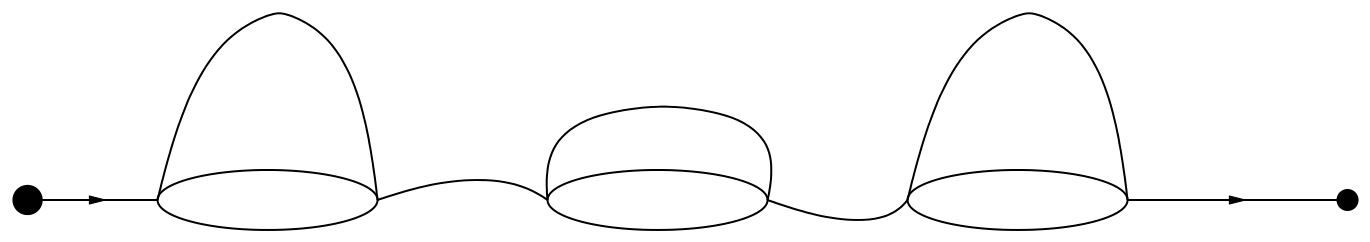
\includegraphics[width=0.68\textwidth]{fig05-pearly.png}
  \caption{Morse–Bott（或“珠串”型）Floer 轨道（原文 Figure~4，第 18 页）。\label{Fig:PearlyGradient}}
\end{figure}

\begin{Example}
环 $HF^*(L,L)$ \emph{并不}总是斜交换的。取 $L = S^1_{eq} \subset \bP^1$；则 $HF^*(L,L) \cong \bC[x]/(x^2=1)$，其中 $|x|=1$ 是最高次生成元，且 $\mu^2(x,x)=1_L$。取珠串模型，该乘积由圆盘 $(D^2, \partial D^2) \rightarrow (\bP^1, S^1_{eq})$ 输出处的取值来定义，这些圆盘带有两个输入标记点，它们是赤道上的固定一般位置点。三个边界标记点有固定的循环次序，由此产生两种可能：若像圆盘是上半球面，取值扫过 $S^1_{eq}$ 上的一条链；若像圆盘是下半球面，则扫过补链。两者合起来构成 $L$ 的基本类。
\end{Example}

\begin{Example} \label{Ex:ToricFibre}
设 $X$ 是单调的，$L\subset X$ 是极小 Maslov 数为 $\mu_L$ 的单调拉格朗日环面。谱序列 $H^*(L) \Rightarrow HF^*(L,L)$ 中的微分 $\partial_1$ 是映射
\begin{equation} \label{Eqn:ToricDifferential}
H^1(L) \longrightarrow H^{2-\mu_L}(L).
\end{equation}
若 $\mu_L=2$ 且该映射非零，则 $H^0(L)$ 中的单位元成为边界，从而在 $HF^*(L,L)$ 中消失，这意味着后者恒为零。若 \eqref{Eqn:ToricDifferential} 为零，则 $H^1(L) \subset \ker(\partial_1)$；由于该核是子环，故 $H^*(L) \subset \ker(\partial_1)$ 且 $\partial_1 \equiv 0$。又因高阶 $\partial_i$ 的次数为 $1-2i \leq -2$，同样的论证表明 $H^1(L)$（从而 $H^*(L)$）位于每个 $\partial_i$ 的核中，这说明谱序列退化。因此，若 $L\subset X$ 是\emph{可移开的}单调环面（例如 $\bC^n$ 中的一个），则由 $HF(L,L)=0$ 可得 $\mu_L = 2$。
\end{Example}

存在一个范畴 Don$(X)$，即 Donaldson 范畴，其对象是（无障碍的）拉格朗日子流形，态射是 Floer 上同调群。合成由全纯三角乘积给出。若 $X$ 是单调的，则该范畴分解为彼此正交的子范畴
\begin{equation} \label{Eqn:DonSplits}
\mathrm{Don}(X) = \bigoplus_{\lambda} \mathrm{Don}(X;\lambda)
\end{equation}
其中 $\lambda$ 取遍 $\frak{m}_0(L)$ 的所有可能值，因为只有当 $\frak{m}_0(L) = \frak{m}_0(L')$ 时，$HF^*(L,L')$ 才对一对拉格朗日有良好定义。由于 $\frak{m}_0(L)$ 计数 Maslov 指标 2 的圆盘，若 $X$ 的极小 Chern 数 $>1$，则任何单连通的拉格朗日都必然落在 Don$(X;0)$ 中。
% [Tutor Note: 分解 \eqref{Eqn:DonSplits} 的依据是 $\frak{m}_0(L)$ 只依赖于单个拉格朗日；
%   两个分支 $\lambda\neq\lambda'$ 之间没有非零态射，故是“正交”直和而非普通直和。
%   注意 $\frak{m}_0(L)$ 是 Novikov 域中的数（计数带面积的 Maslov 2 圆盘），
%   因此分解的指标集 $\lambda$ 是连续取值的；这与按拓扑不变量进行的离散分解不同。]

\subsubsection{模结构}\label{Subsec:ModuleStructures}

Floer 上同调 $HF^*(L, L')$ 是有单位元环 $HF^*(L,L)$ 上的右模。此外还有量子上同调作用的模结构：对任何（可定向的）拉格朗日 $L$，存在有单位元的环同态
\begin{equation} \label{Eqn:ClosedOpen}
\mathcal{CO}^0: QH^*(X) \longrightarrow HF^*(L,L)
\end{equation}
称为（闭-开弦映射的长度零部分）。它通过计数以 $L$ 为边界的全纯圆盘来定义：圆盘带一个内部输入标记点，该点被约束在 $X$ 中代表某个 $QH^*$-生成元的闭链上；另有一个边界标记点，我们在该点取值以定义输出的 Floer 类。$QH^*(X)$ 是交换的，且 $\mathcal{CO}^0$ 的像落在 $HF^*(L,L)$ 的中心。

\begin{Example}
$\bC\bP^n$ 的量子上同调为 $\Lambda[x]/(x^{n+1}=1)$，其中 $|x|=2$。设 $L\subset \bC\bP^n$ 是拉格朗日子流形。若 $HF^*(L,L)$ 有良好定义，则由 $x$ 在 $HF^*(L,L)$ 中的像可逆可知，后者必须是 2-周期的。
\end{Example}

Auroux、Kontsevich 与 Seidel 的一个美妙观察 \cite{Auroux} 是：在单调情形下、并避开特征 2，映射 \eqref{Eqn:ClosedOpen} 把 $c_1(X) \mapsto \frak{m}_0(L) e_L$，这意味着 \eqref{Eqn:DonSplits} 中出现的值 $\lambda$ 恰好是自同态 $\ast c_1(X)$ 作用在 $QH^*(X)$ 上的特征值。简短讨论见注 \ref{Rem:StarC1}。
% [Tutor Note: $\frak{m}_0(L)$ 与量子上同调的联系是本节的深层要点：闭-开弦映射把
%   $QH^*(X)$（由 $X$ 的 Gromov–Witten 理论决定）送到 $HF^*(L,L)$，而 $c_1(X)$ 的像
%   正是 “Maslov 2 圆盘计数” $\frak{m}_0(L)$ 乘以单位元 $e_L$。因此 $\frak{m}_0(L)$
%   不是自由参数，而必须等于 $\ast c_1(X)$ 在 $QH^*(X)$ 上的某个特征值——
%   这正是 \eqref{Eqn:DonSplits} 中 $\lambda$ 的取值有限（离散）的原因。
%   易错点：$c_1\mapsto\frak{m}_0(L)e_L$ 成立需要“单调 + 特征 $\neq 2$”；
%   $e_L$ 是 $HF^*(L,L)$ 的单位元，而 $\frak{m}_0(L)\in\Lambda$ 属系数域。]

\subsubsection{正合三角\label{Subsec:ExactTriDon}}

暂且这样定义：三个拉格朗日子流形与态射
\[
\xymatrix{ L \ar^{a}[r] & L' \ar^{b}[r] & \ar@/^1.5pc/[ll]_{[1]} L''}
\]
在 Don$(X)$ 中构成一个\emph{正合三角}，如果对任意另一个拉格朗日 $K$，与给定态射（Floer 闭链）作复合诱导出 Floer 上同调群的长正合列
\[
\cdots  \rightarrow HF^i(K,L) \stackrel{a}{\longrightarrow} HF^i(K,L')\stackrel{b}{\longrightarrow} HF^i(K,L'') \rightarrow HF^{i+1}(K,L) \rightarrow \cdots.
\]
也许令人惊讶的是，正合三角确实存在：
% [Tutor Note: “正合三角”在这里是由 Yoneda 型条件定义的：对每个测试对象 $K$，
%   $HF^*(K,\cdot)$ 把三角 $L\to L'\to L''$ 变成长正合列；并非三角本身在链层次
%   正合。弧上的 $[1]$ 表示映射锥的平移，方向（逆时针）也是约定的一部分，
%   画反会改变三角的定向。]

\hspace{1em} $\bullet$ 若 $L \pitchfork L' = \{p\}$ 横截相交于唯一一点，且 $L'' = L\# L'$ 是 Lagrange 手术 \cite{Polterovich}（拓扑上即连通和：把二重点的邻域 $\bR^n \cup i\bR^n$ 换成一个拉格朗日 1-柄 $S^{n-1} \times \bR$），则 \cite{BiranCornea2, FO3} 存在正合三角 $L \stackrel{p}{\longrightarrow} L' \longrightarrow L''$。在图 \ref{Fig:SurgeryTriangle} 中，直的拉格朗日 $L, L'$ 的交点从左至右被消解；虚线弧是第三个拉格朗日 $K$；可以看到右图中有两个全纯圆盘对复形 $CF^*(K, L\#L')$ 作出贡献，一个来自复形 $CF^*(K,L)$，另一个来自与 $p$ 的乘法（把该点视为映射 $CF(K,L) \rightarrow CF(K,L')$），这示意性地给出拟同构
\[
CF(K,L\#L') \stackrel{\sim}{\longrightarrow} \left( CF(K,L) \oplus CF(K,L'), \left(\begin{array}{cc} \partial_L & 0 \\ \mu^2(p,\cdot) & \partial_{L'} \end{array} \right)\right)
\]
（在更高维情形，从刚性全纯三角形的集合到以 $K$ 与 $L\#L'$ 为边界的刚性圆盘的相应单射并非平凡）。
% [Tutor Note: 右端矩阵微分的非对角项 $\mu^2(p,\cdot)$ 是符号与次序的双重易错点：
%   它把 $CF(K,L)$ 送到 $CF(K,L')$，其中 $p\in CF(L,L')=HF^*(L,L')$ 充当“较晚”的
%   变元；若把 $p$ 放进第二个变元或漏掉分次符号 $(-1)^{|p|+1}$ 型因子，
%   $\partial^2=0$ 会失效，且手术三角的定向随之出错。对角块是 $\partial_L,\partial_{L'}$，
%   次序对应直和分解 $CF(K,L)\oplus CF(K,L')$，不要与上三角/下三角混淆。]

\begin{figure}[ht]
  \centering
  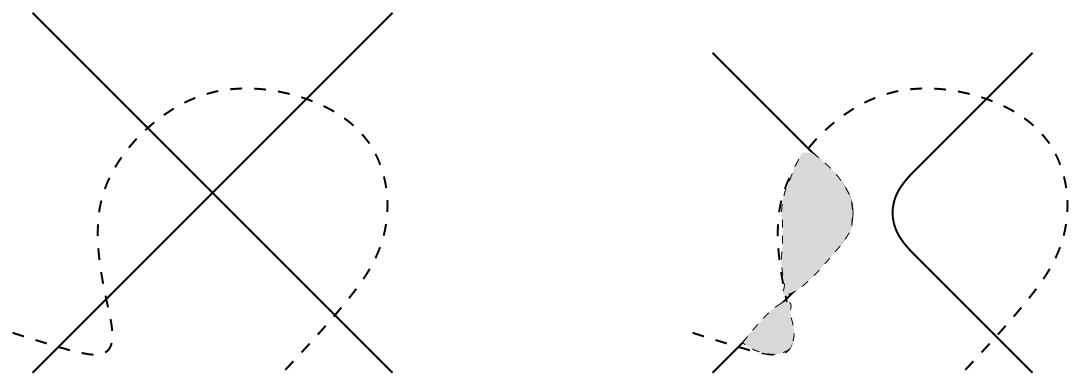
\includegraphics[width=0.5\textwidth]{fig06-surgery-tri.png}
  \caption{走向手术正合三角（原文 Figure~5，第 20 页）。\label{Fig:SurgeryTriangle}}
\end{figure}

% 原文此处有 \newcommand{\ev}{\mathrm{ev}}；本译稿的导言区已定义 \ev，故略去以免重复定义报错。

\hspace{1em} $\bullet$ 若 $V\cong S^n \subset X$ 是（单调或恰当的）拉格朗日球面，$\tau_V$ 表示沿 $V$ 的 Dehn 扭转，则 \cite{Seidel:LES} 在 Don$(X)$ 的加法扩张中存在正合三角 $L \stackrel{\phi}{\longrightarrow} \tau_V(L) \rightarrow HF^*(V,L)\otimes V$；所谓加法扩张，就是我们形式地允许对象的直和，或等价地允许拉格朗日与分次向量空间作张量积。固定任意另一个拉格朗日 $K$。首先把 $K \cap \tau_V(L)$ 的交点与 $K \cap L$ 的点（我们假定这些点位于 $\tau_V$ 的支集之外）等同起来，再对 $V \cap L$ 的每个点附加一份 $K \cap V$，因为每当 $L$ 与 $V$ 相交，$\tau_V$ 就把 $L$ 绕 $V$ 缠绕一圈。于是在向量空间层次上
$CF(K,\tau_V(L))  = CF(K,L) \oplus (CF(V,L)\otimes CF(K,V))$。态射 $\phi$ 计数 $D^2\backslash \{-1\}$ 上 Lefschetz 纤维化的截面，该纤维化在 $0$ 处有一个临界点（消没圈 $V$ 在那里被收缩为一点），边界条件为 $L, \tau_V(L)$。所需的同伦
\begin{equation} \label{Eqn:Nullhtpy}
\kappa: CF(V,L) \rightarrow CF(V,\tau_V(L)), \quad \partial \kappa \pm \kappa \partial + \mu^2(\phi, \cdot) = 0
\end{equation}
由如图 \ref{Fig:LESnullhtpy} 的一族单参数 Lefschetz 纤维化得到，并由此给出长正合列。左端看到的是复合 $\mu^2(\phi,\cdot)$；图中最右的纤维化没有刚性截面，因为模型 Lefschetz 纤维化 $\bC^{n+1} \rightarrow \bC$ 在以已经冒泡的消没圈 $V$ 为边界条件时\emph{没有}这样的截面——模型的所有截面模空间的虚维数都是奇数。因此，若 $\kappa$ 计数整个族中的刚性曲线，就得到 \eqref{Eqn:Nullhtpy}。把 $\kappa$ 视为映射 $CF(V,L)\otimes V \rightarrow \tau_V(L)$，并令 $\ev: CF(V,L) \otimes V \rightarrow L$ 为自然的取值映射，则 \eqref{Eqn:Nullhtpy} 表明 $\mu^2(\phi,\ev)$ 经 $\kappa$ 零伦，从而按需把 Cone$(\ev)$ 与 $\tau_V(L)$ 等同起来。
% [Tutor Note: \eqref{Eqn:Nullhtpy} 里的 $\pm$ 号取决于定向与分次约定，原文有意保留
%   未定；核对时应把 $\kappa$ 的度数与 $\mu^2(\phi,\cdot)$ 的度数一起检查，才能确定
%   是 $+$ 还是 $-$。几何上，$\kappa$ 是一族 Lefschetz 纤维化的刚性截面计数：
%   左端的纤维化给出 $\mu^2(\phi,\cdot)$，右端因模型纤维化的截面模空间虚维数为奇而
%   无刚性截面，于是整族的计数恰好给出零伦。另有一步易漏：把 $\kappa$ 视为
%   $CF(V,L)\otimes V\to\tau_V(L)$ 时要用取值映射 $\ev$ 与 $\mu^2$ 的配对。]

\begin{figure}[ht]
  \centering
  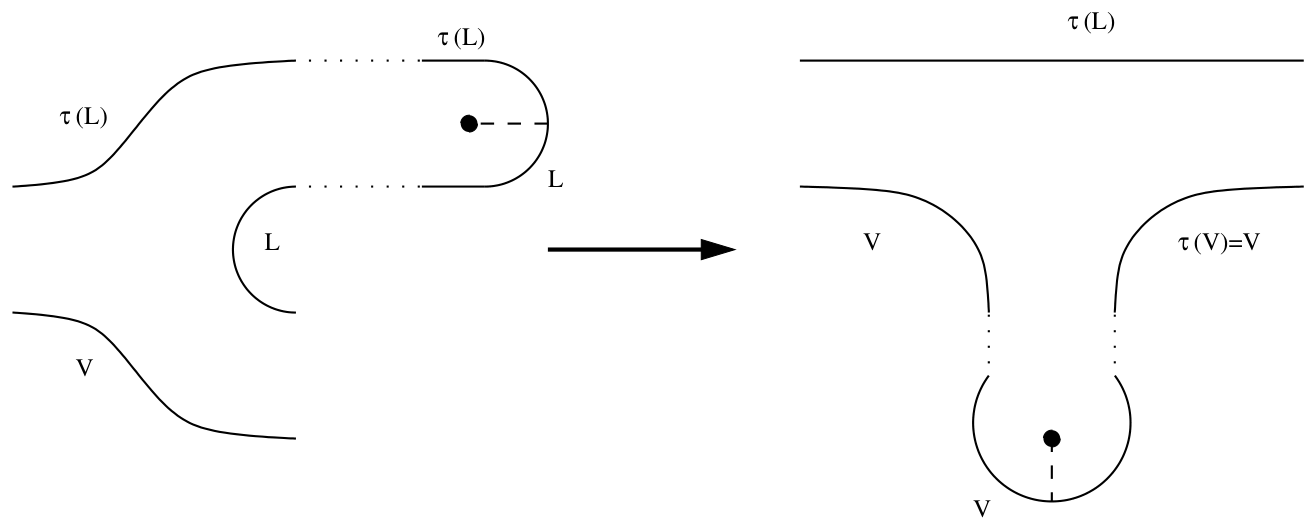
\includegraphics[width=0.7\textwidth]{fig07-les-nullhtpy.png}
  \caption{走向 Dehn 扭转正合三角（原文 Figure~6，第 21 页）。\label{Fig:LESnullhtpy}}
\end{figure}

\subsubsection{来自对应的函子}\label{Sec:Quilt}

记 Don$^{\#}(Y)$ 为 $Y$ 的广义拉格朗日子流形范畴，其对象是拉格朗日对应的序列
\[
\{pt\} \stackrel{L_0}{\longrightarrow} Y_0 \stackrel{L_{01}}{\longrightarrow} \cdots \stackrel{L_{k-1,k}}{\longrightarrow} Y_k = Y
\]
其中 $L_{i,i+1} \subset Y_i^- \times Y_{i+1}$ 是拉格朗日子流形。这里 $(Y,\omega_Y)^- = (Y, -\omega_Y)$。Wehrheim 与 Woodward \cite{WW1, WW2} 把 Floer 上同调（本质上是形式地）推广到广义拉格朗日对。例如给定 $L \subset X$、$K\subset Y$ 与 $\Gamma \subset Y^- \times X$，$HF(L, (\{pt\} \stackrel{K}{\longrightarrow} Y \stackrel{\Gamma}{\longrightarrow} X))$ 按定义就是在 $Y^- \times X$ 中计算的 $HF(K \times L, \Gamma)$。Floer 乘积到广义拉格朗日的推广更为复杂，涉及对“quilt 化”黎曼曲面的计数（这类曲面的内部接缝标以拉格朗日边界条件）。设 $(X,\omega_X)$ 与 $(Y,\omega_Y)$ 是辛流形，$\Gamma \subset X^-\times Y$ 是拉格朗日对应，其中 $X^-$ 表示 $(X,-\omega)$。在强单调性假设下，$\Gamma$ 诱导函子
\[
\Phi_{\Gamma}: \mathrm{Don}(X) \longrightarrow \mathrm{Don}^{\#}(Y),  \qquad  \Phi_{\Gamma}: L \, \mapsto \,  \left( \{pt\} \stackrel{L}{\longrightarrow} X \stackrel{\Gamma}{\longrightarrow} Y\right)
\]
它在对象上按所示拼接方式作用。Wehrheim 与 Woodward 的一个重要而困难的定理是：若几何复合
\[
\Gamma \circ L \ = \ \left\{ u \in Y \ \big| \ (x,u) \in \Gamma \ \mathrm{for \ some} \ x\in L\, \right\}
\]
是嵌入的拉格朗日子流形，则 $\Phi_{\Gamma}(L)$ 与 $\Gamma\circ L$ 在 Don$^{\#}(Y)$ 中同构（特别地，形式复合与通常 Donaldson 范畴中的某个对象同构）。利用 quilt 理论，可以构造一个底层的函子
\begin{equation} \label{Eqn:QuiltFunctor}
\Phi: \mathrm{Don}(X^- \times Y) \longrightarrow \mathrm{Fun}(\mathrm{Don}(X), \mathrm{Don}^{\#}(Y))
\end{equation}
其中 $\Phi: \Gamma \mapsto \Phi_{\Gamma}$。特别地，若 $HF(\Gamma,\Gamma) = 0$（在 $X^-\times Y$ 中计算），则 $\Phi_{\Gamma}$ 是零函子；而若 $\Phi_{\Gamma}(L) \neq 0$，则 $\Gamma \neq 0$。
% [Tutor Note: 函子 \eqref{Eqn:QuiltFunctor} 的“形式化”之处要分清两个层次：
%   对象上只是把对应 $\Gamma$ 拼接到 $L$ 后面（符号记法），真正的函子性依赖 quilt
%   模空间的计数——即带内部接缝（标以拉格朗日边界条件）的黎曼曲面的全纯映射。
%   Wehrheim–Woodward 定理的实质是：当几何复合 $\Gamma\circ L$ 是嵌入子流形时，
%   形式复合 $\Phi_{\Gamma}(L)$ 与它在 $\mathrm{Don}^{\#}(Y)$ 中同构，从而“形式”范畴
%   并不比几何范畴更病态。注意 $\mathrm{Don}^{\#}$ 的对象是序列而非单个流形。]

\begin{Example} \label{Ex:Corr}
参见 \cite{WW2}。记 $S^3 \subset \bC^2$ 为单位球面。Hopf 映射 $h: S^3 \rightarrow S^2$ 满足 $(\omega_{\st})|_{S^3} = h^*(\omega_{\operatorname{FS}})$。复合 $(\mathrm{antipodal})\circ h$ 的图定义了 $B^4(r) \times \bP^1$ 的拉格朗日子流形（对任意 $r>1$），从而得到带单调辛形式的拉格朗日子流形 $\Gamma=S^3 \subset \bP^2 \times \bP^1$。把 $\Gamma$ 视为从 $\mathrm{Don}(\bP^1)$ 到 $\mathrm{Don}^{\#}(\bP^2)$ 的函子。像 $\Phi_{\Gamma}(S^1_{eq})$ 拟同构于 $\bP^2$ 中的 Clifford 环面。由例 \ref{Ex:ToricFibre} 可知它具有非平凡的自 Floer 上同调，这意味着 $HF(\Gamma,\Gamma) \neq 0$。
\end{Example}

初看之下，过渡到 Don$^{\#}(Y)$ 稍显吓人：其定义涉及中间辛流形的任意序列，似乎难以驾驭。然而，给定有限个拉格朗日 $\{L_i\} \subset Y$ 及相应的代数 $A = \oplus_{i,j} HF^*(L_i, L_j)$，存在一个函子 Don$^{\#}(Y) \rightarrow \mathrm{mod}$-$(A)$，它把任一广义拉格朗日送到它与诸 $L_i$ 的 Floer 上同调之直和；这使人得以把非交换代数的工具用于这个扩张范畴。
% [Tutor Note: 这里的 $A=\oplus_{i,j}HF^*(L_i,L_j)$ 只记录了对象之间的 Floer 群，
%   还不含高阶运算；函子 $\mathrm{Don}^{\#}(Y)\to\mathrm{mod}$-$A$ 是“取与诸 $L_i$
%   的 Floer 上同调”的直和，属于 Yoneda 型构造。它在观念上把几何范畴嵌入
%   非交换代数，但丢失了 $A_\infty$ 的高阶信息——这正是 §4 要补上的结构。]

\subsection{应用 II}

我们简要说明迄今引入的代数结构如何扩大理论的适用范围；这些例子取自 \cite{Buhovsky} 与 \cite{Smith:HFQuadrics}。

\subsubsection{附近的拉格朗日}

设 $L \subset T^*S^{2k+1}$ 是恰当拉格朗日，且 $H_1(L;\bZ) = 0$。我们断言 $H^*(L) \cong H^*(S^{2k+1})$。如例 \ref{Ex:Corr} 那样，Hopf 映射
\[
\bC^{k+1}\backslash \{0\} \supset S^{2k+1} \stackrel{h}{\longrightarrow} \bP^k
\]
由取射影化给出，其性质是 $h^*\omega_{\operatorname{FS}} = (\omega_{\st})|_{S^{2k+1}}$。因此，取图可得到拉格朗日嵌入 $S^{2k+1} \subset \bC^{k+1} \times (\bP^k)^-$。如有必要把 $L\subset T^*S^{2k+1}$ 缩放使其靠近零截面，则 $L$ 也嵌入这一乘积中。由假设 $H_1(L;\bZ) = 0$，该嵌入是单调的，因此 $HF(L,L)$ 有良好定义，在乘积 $\bC^{k+1} \times (\bP^k)^-$ 中计算。由于可在第一个因子上作平移，它显然可以被移开自身，故 $HF(L,L)=0$。

现在考虑 Oh 谱序列，即命题 \ref{Lem:Oh}。$L$ 在 $T^*S^{2k+1}$ 中的 Maslov 类为零，但在 $\bC^{k+1} \times (\bP^k)^-$ 中的极小 Maslov 数为 $2k+2$。这意味着 Oh 谱序列中唯一非平凡的微分形如
\[
H^{i+2k+1}(L) \rightarrow H^i(L) \rightarrow H^{i-2k-1}(L) \qquad \forall \ 0 \leq i \leq 2k+1.
\]
所需结论随即得到。

\subsubsection{映射类群}

设 $S$ 是亏格 2 的闭曲面，$p
\in S$，而 $\scrM(S)$ 是把边界环路送到 $-I$ 的表示 $\pi_1(S\backslash \{p\})$ 到 $SU(2)$ 的共轭类的模空间。它是辛的，因为它是秩二丛 $E \rightarrow S$ 上联络的无穷维空间的商，而后者带有自然辛形式 $\omega(a,b) = \int_S \tr(a \wedge b)$，其中 $a,b \in \Omega^1(S;\End(E))$。固定 $p$ 不动的 $S$ 的微分同胚构成映射类群 $\Gamma(S,p)$，它辛地作用在 $\scrM(S)$ 上；我们断言，对任意 $\phi \in \Gamma(S,p)$，都有 $HF^*(\phi) \neq \{0\}$。

证明的核心是如下归纳论证。同调本质的简单闭曲线 $\gamma \subset S$ 通过取沿 $\gamma$ 和乐平凡的联络，定义了拉格朗日 3-球面 $SU(2) \cong L_\gamma \subset \scrM(S)$。Dehn 扭转 $\tau_\gamma \in \Gamma(S,p)$ 通过高维 Dehn 扭转 $\tau_{L_{\gamma}}$ 作用在 $\scrM(S)$ 上。空间 $\scrM(S)$ 是单调的，极小 Chern 数为 2，且 Spec$(\ast c_1: QH^*(\scrM(S)) \rightarrow QH^*(\scrM(S)))$ 为 $\{0, \pm 4i\}$。存在正合三角
\begin{equation} \label{Eqn:InductiveTriangle}
\xymatrix{ HF^*(\phi) \ar[r] & HF^*(\tau_{L_\gamma} \circ \phi)  \ar[r] & \ar@/^1.5pc/[ll]^{[1]} HF^*(L_{\gamma}, \phi(L_{\gamma}))}
\end{equation}
对任意 $\phi \in \Gamma(S,p)$ 与本质曲线 $\gamma \subset S$ 成立。考虑特征值 $4i$ 的相应广义特征空间所构成的正合三角。由于 $c_1 \mapsto \frak{m}_0(L_{\gamma}) \in HF^*(L_{\gamma}, L_{\gamma}) = A$，且 $L_{\gamma}$ 的极小 Maslov 数 $>2$，故 $c_1$ 在 $A$ 上平凡地作用，从而在 $A$-模 $HF^*(L_{\gamma}, \phi(L_{\gamma}))$ 上平凡地作用。由此可知，特征值 $4i$ 的 $\ast c_1$-广义特征空间在复合 $\tau_{L_{\gamma}}$ 下不变；类似的论证表明它在复合逆 Dehn 扭转下也不变。由于这类扭转生成映射类群，归纳地只需证明相应特征空间对 $HF^*(\id)\cong QH^*(\scrM(S))$ 非零。Newstead 的一个定理 \cite{Newstead} 把 $\scrM(S)$ 等同于 $\bP^5$ 中两个二次超曲面的交，由此 $QH^*$ 的计算是直接的 \cite{SKD}：$4i$-广义特征空间的秩为 1。

一个推论是：若 $Y \rightarrow S^1$ 是由亏格 2 曲线纤维化的任意 3-流形，则 $\pi_1(Y)$ 容许非阿贝尔的 $SO(3)$-表示。
% [Tutor Note: 正合三角 \eqref{Eqn:InductiveTriangle} 的直观是：沿本质曲线 $\gamma$ 作
%   高维 Dehn 扭转 $\tau_{L_\gamma}$ 不改变 $\ast c_1$-广义特征空间；而这类扭转生成
%   映射类群，故只须验证恒等映射这一情形。易错点：$\frak{m}_0(L_\gamma)$ 在
%   $HF^*(L_\gamma,L_\gamma)=A$ 中是单位元的倍数，因此 $c_1$ 在 $A$ 上的作用是
%   “乘以常数”，它在 $A$-模上仍是常数倍——这一步用到了 $L_\gamma$ 的极小 Maslov
%   数 $>2$（否则 $\frak{m}_0$ 不再只由单位元贡献）。]

\subsection{不足}\label{Subsec:Shortcoming}

下述情形经常出现：给定的辛流形 $X$ 含有某个有限的“区分”拉格朗日子流形族，人们期待通过迭代地取态射的锥（例如通过 Lagrange 手术，或取 Dehn 扭转下的像）来生成所有拉格朗日。这有限族拉格朗日 $\{L_i\}$ 定义一个环
\[
A = \oplus_{i,j} HF^*(L_i, L_j)
\]
而任何其他拉格朗日 $K$ 定义一个右 $A$-模
\[
Y_K = \oplus_i HF^*(L_i, K).
\]
现在给定两个拉格朗日 $K, K'$，可以考虑两个显然的群：一个是几何地定义的 Floer 上同调 $HF^*(K,K')$，另一个是代数地定义的态射群 $\Ext_{A-mod}^*(Y_K, Y_{K'})$。就目前发展出的结构而言，即便 $\{L_i\}$ “应当生成”的直觉是正确的，这两个群通常也不会相同。

\begin{figure}[ht]
  \centering
  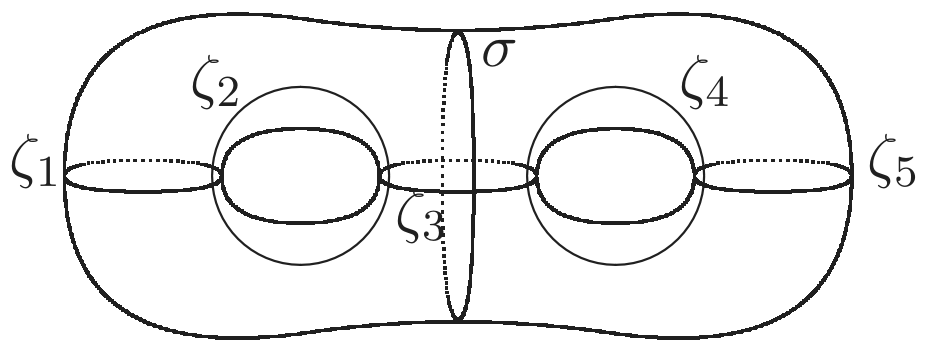
\includegraphics[width=0.45\textwidth]{fig08-genus2.png}
  \caption{亏格 2 曲面；图中标出曲线 $\zeta_1$、$\zeta_2$、$\zeta_3$、$\zeta_4$、$\zeta_5$ 与 $\sigma$（原文 Figure~7，第 23 页）。\label{Fig:genus2pencil}}
\end{figure}

\begin{Example}
考虑亏格 2 曲面。曲线 $\zeta_i$ 生成所有简单闭曲线，意思是任何同伦本质的曲线必与某个 $\zeta_i$ 有非平凡的几何相交数；且 Dehn 扭转 $\tau_{\zeta_j}$ 生成映射类群\footnote{由命题 \ref{Prop:SpheresGenerate} 可知，曲线 $\zeta_i$ 分裂生成 Fukaya 范畴。}。在环 $A = \oplus_{i,j} HF^*(\zeta_i, \zeta_j)$ 上，由曲线 $\sigma$ 定义的模 $Y_{\sigma}$ 同构于 $\zeta_3$ 上的单模与其平移之和 $\hat{Y}_{\sigma} = S_{\zeta_3} \oplus S_{\zeta_3}[1]$，这本质上是因为图中没有非常值的全纯月牙或三角形。然而，$S_{\zeta_3} \oplus S_{\zeta_3}[1]$ 的自同态代数是矩阵代数，特别地 Ext$_{A-\mathrm{mod}}(\hat{Y}_{\sigma}, \hat{Y}_{\sigma}) \not \cong HF^*(\sigma,\sigma) = H^*(S^1)$。
\end{Example}

问题在于：$A$ 并不只是一个环；把它仅仅当作环，就忽略了重要的结构——我们下面引入该结构。
% [Tutor Note: 本例是 §3.8 的核心：$\Ext_A$ 与 $HF^*$ 的差异不是技术性误差，而是
%   因为 $A$ 缺少 $A_\infty$ 的高阶运算。$Y_\sigma\cong S_{\zeta_3}\oplus S_{\zeta_3}[1]$
%   之所以成立，是由于图中没有非常值的全纯月牙/三角形；而矩阵代数的自同态群
%   比 $HF^*(\sigma,\sigma)=H^*(S^1)$ 大，说明“只记住环 $A$”会丢失信息。
%   这是下一节引入 Fukaya 范畴（$A_\infty$-结构）的直接动机。]

\begin{Notes}
关于 Floer（与量子）上同调的基础，参见 \cite{Floer, Oh, AudinDamian, McD-S2}。关于代数结构，参见 \cite{BiranCornea, FO3, WW2, RitterSmith}，以及 Seidel 的许多论文，例如 \cite{Seidel:graded, Seidel:MCG, Seidel:LES, Seidel:twist}。
\end{Notes}



%%%%%%%%%%%%%%%%%%%%%%%%%%%%%%%%%%%%%%%%%%%%%%%%%%%%%%%%%%%%%%%%%%%%%%%%%%%%%%%
%%  [Inlined] s04a-fukaya
%%%%%%%%%%%%%%%%%%%%%%%%%%%%%%%%%%%%%%%%%%%%%%%%%%%%%%%%%%%%%%%%%%%%%%%%%%%%%%%
%%%%%%%%%%%%%%%%%%%%%%%%%%%%%%%%%%%%%%%%%%%%%%%%%%%%%%%%%%%%%%%%%%%%%%%%%%%%%%%
%  s04a-fukaya.tex —— 第 4 节 The Fukaya category（§4.1–§4.4）
%  原文：Ivan Smith, \emph{A Symplectic Prolegomenon}, arXiv:1401.0269v2
%        源码第 963–1164 行（原文第 24–29 页）
%  说明：本节只含 §4 的前半部分；§4.5 起由 s04b-fukaya.tex 接续。
%%%%%%%%%%%%%%%%%%%%%%%%%%%%%%%%%%%%%%%%%%%%%%%%%%%%%%%%%%%%%%%%%%%%%%%%%%%%%%%

\section{Fukaya 范畴}\label{Sec:Fukaya}

\begin{keypoints}
\begin{itemize}
  \item \textbf{核心图像}：Fukaya 范畴 $\scrF(X)$ 以恰当或单调的拉格朗日子流形为对象、以 Floer 上同调群为态射空间，并用全纯圆盘的计数定义 $A_{\infty}$ 复合；它是拉格朗日相交数理论的范畴化。
  \item \textbf{关键工具}：$A_{\infty}$ 关系的树图（mangrove）表述、Stasheff 结合面体与 Deligne--Mumford 紧化、扭曲复形与幂等完备化。
  \item \textbf{结构结论}：链水平的 $\mu^2$ 只结合到同伦，高阶运算 $\mu^d$（$d\ge 3$）不是链映射、也不下传到上同调；只有在 $H(\scrA)$ 上才恢复通常的范畴结构。
  \item \textbf{三角结构}：$A_{\infty}$-模的映射锥、扭曲复形 $\Tw(\scrA)$ 及其幂等完备化给出导出范畴 $D^\pi(\scrA)$，它既三角又幂等完备。
  \item \textbf{扭转}：扭转变换 $\scrT_Y$ 是沿求值态射 $\scrM(Y)\otimes\scrY\to\scrM$ 的锥；当 $L$ 为拉格朗日球面时，Seidel 定理断言代数扭转 $\scrT_L$ 与几何正 Dehn 扭转 $\tau_L$ 拟同构。
  \item \textbf{与后文联系}：这套代数机器（Hochschild 上同调、生成性判据、扭转函子）将在 §4.5 及第 5、6 节中用于具体计算各类流形的 Fukaya 范畴。
\end{itemize}
\end{keypoints}

\subsection{$A_{\infty}$-范畴}

域 $\bK$ 上的（非幺）$A_{\infty}$-范畴 $\scrA$ 由以下数据构成：一个对象集 Ob$\,\scrA$；对每对 $X_0, X_1 \in$ Ob$\,\scrA$ 一个（依情形为 $\bZ_2$-分次或 $\bZ$-分次的）$\bK$-向量空间 $hom_{\scrA}(X_0, X_1)$；以及对 $k \geq 1$ 的 $\bK$-线性复合映射
\[
\mu_{\scrA}^k: hom_{\scrA}(X_{k-1},X_k) \otimes \cdots \otimes hom_{\scrA}(X_0,X_1) \longrightarrow hom_{\scrA}(X_0,X_k)[2-k]
\]
其次数为 $2-k$（记号 $[l]$ 指\emph{向下}平移 $l \in \bZ$，或依情形 $l\in \bZ_2$）。映射族 $\{\mu^k\}$ 满足一列二次方程
\[
\sum_{m,n} (-1)^{\maltese_n} \mu_{\scrA}^{k-m+1} (a_d,\ldots,a_{n+m+1}, \mu_{\scrA}(a_{n+m},\ldots,a_{n+1}),a_n \ldots, a_1) = 0
\]
其中 $\maltese_n = \sum_{j=1}^n |a_j|-n$，$|a|$ 表示 $a$ 的次数，而求和遍历所有可能的复合方式：$1 \leq m \leq k$，$0\leq n \leq k-m$。
% [Tutor Note: 这是 $A_\infty$ 关系中最易出符号错的地方：指数 $\maltese_n=\sum_{j=1}^n|a_j|-n$ 中的 $-n$ 项不可漏，它保证 $\mu^k$ 的总次数恰为 $2-k$；不同文献（如 Seidel 的书）对 $(-1)$ 的指数有不同但等价的写法，核对时请以本式的求和范围 $1\le m\le k$、$0\le n\le k-m$ 为准。]
这些方程特别蕴含 $hom_{\scrA}(X_0,X_1)$ 是以 $\mu^1_{\scrA}$ 为微分的上链复形；上同调范畴 $H(\scrA)$ 与 $\scrA$ 有相同的对象，但其态射群取上述上链复形的上同调。$H(\scrA)$ 带有结合的复合
\[
[a_2]\cdot[a_1] = (-1)^{|a_1|}[\mu_{\scrA}^2(a_2,a_1)]
\]
而 $\scrA$ 链水平的复合 $\mu_{\scrA}^2$ 只结合到同伦。（因此 $\scrA$ 实际上并不是一个范畴。）更具体地说，若 $x,y,z$ 满足 $\mu^1(\cdot) = 0$，则在 $\scrA$ 中有
\[
\mu^1\mu^3(x,y,z) + \mu^2(x,\mu^2(y,z)) + \mu^2(\mu^2(x,y),z) = 0.\]
% [Tutor Note: 注意 $\mu^2$ 的输入次序是 $(a_2,a_1)$ 而乘积写作 $[a_2]\cdot[a_1]$，并带符号 $(-1)^{|a_1|}$；若把次序或符号记反，下式结合性恒等式的符号就对不上——这是核对 $A_\infty$ 约定时最省时的检验点。]
高阶复合 $\mu_{\scrA}^d$ \emph{不是}链映射，也不下传到上同调。只有一个对象的 $A_{\infty}$-范畴就是 $A_{\infty}$-代数。

\begin{Example}
拓扑空间 $Q$ 的带基点环路空间的奇异链复形 $C_*(\Omega Q)$ 是一个 $A_{\infty}$-代数，这反映了 $\Omega Q$ 是 $h$-空间这一事实：由环路拼接给出的复合只结合到一族高阶同伦。
\end{Example}

非幺 $A_{\infty}$-范畴 $\scrA$ 与 $\scrB$ 之间的非幺 $A_{\infty}$-函子 $\cF: \scrA \rightarrow \scrB$ 包含一个对象映射 $\cF$: Ob$\,\scrA \rightarrow$ Ob$\,\scrB$，以及 $d\geq 1$ 的多重线性映射
\[
\cF^d: hom_{\scrA}(X_{d-1}, X_d) \otimes \cdots \otimes hom_{\scrA}(X_0,X_1) \rightarrow hom_{\scrB}(\cF X_0, \cF X_d)[1-d]
\]
它们现在满足多项式方程
\begin{multline*}
\sum_{r} \sum_{s_1+\cdots+s_r=d} \mu_{\scrB}^r(\cF^{s_r}(a_d,\ldots,a_{d-s_r+1}),\ldots, \cF^{s_1}(a_{s_1},\ldots, a_{1})) \\
\quad  = \ \sum_{m,n} (-1)^{\maltese_n} \cF^{d-m+1}(a_d,\ldots, a_{n+m+1}, \mu_{\scrA}^m (a_{n+m},\ldots, a_{n+1}), a_{n},\ldots a_1)
\end{multline*}
% [Tutor Note: 函子方程左端对 $r$ 与 $s_1+\cdots+s_r=d$ 的分拆求和（先在 $\scrB$ 中复合），右端对 $m,n$ 求和（先在 $\scrA$ 中复合），两端的组合计数并不相同，这正是树图（mangrove）图示所要表达的内容；初学时最易把两重求和的范围搞混。]
任何这样的数据都定义一个函子 $H(\cF):H(\scrA) \rightarrow H(\scrB)$，其作用为 $[a] \mapsto [\cF^1(a)]$。若 $H(\cF)$ 是同构，则称 $\cF$ 为\emph{拟同构}。$\scrA$ 到 $\scrB$ 的 $A_{\infty}$-函子类构成一个非幺 $A_{\infty}$-范畴 $\scrQ=nu$-$fun(\scrA,\scrB)$ 的对象，见 \cite{FCPLT}。
若把 $A_{\infty}$-运算（多输入、单输出）画成一棵树，则 $A_{\infty}$-关系就是对 图~\ref{Fig:Ainftytree} 顶行右侧那类图像求和。按这套语言，若函子运算像 图~\ref{Fig:Ainftytree} 左下那棵红树（mangrove，部分浸没在水中的树），则函子关系就是对右下那类图像求和。

\begin{figure}[ht]
  \centering
  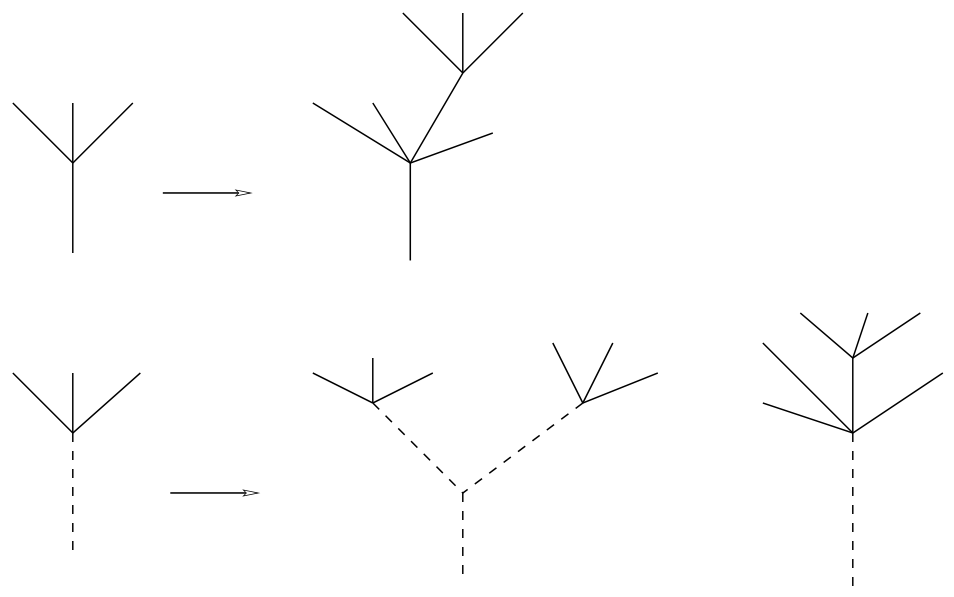
\includegraphics[width=0.6\textwidth]{fig09-ainfty-tree.png}
  \caption{$A_\infty$-关系（上）与 $A_{\infty}$-函子关系（下）是图中右侧所示的一类复合之和（原文 Figure~8，第 25 页）。\label{Fig:Ainftytree}}
\end{figure}

\begin{Remark} \emph{严格幺}的 $A_{\infty}$-范畴 $\scrA$ 是指：对每个对象 $X$ 都有单位元 $e_X \in hom^0_{\scrA}(X,X)$，使得这些 $e_X$ 都是闭的，即 $\mu^1_{\scrA}(e_X)=0$，并且
\[
\mu^2_{\scrA}(a,e_X) = a = (-1)^{|a|}\mu^2_{\scrA}(e_X, a), \quad \mu^k_{\scrA}(\ldots, e_X, \ldots) = 0 \ \forall \, k\geq 3.
\]
若 $H(\scrA)$ 是幺的，即 $H(\scrA)$ 是通常意义下的线性范畴，则称 $\scrA$ 为\emph{上同调幺}的。任何上同调幺的 $A_{\infty}$-范畴都拟同构于一个严格幺的 $A_{\infty}$-范畴 \cite{FCPLT}。
% [Tutor Note: 这里右单位与左单位相差符号：$\mu^2(a,e_X)=a$ 而 $\mu^2(e_X,a)=(-1)^{|a|}a$，这是分次约定下的必然结果；再加上 $\mu^k(\ldots,e_X,\ldots)=0\ (k\geq 3)$ 才得到“严格”单位。对照 §4.3 末可知 Fukaya 范畴一般只在上同调意义下幺。]
\end{Remark}

\subsection{$A_{\infty}$-模与扭曲复形}

$A_{\infty}$-模 $\scrM$ 是范畴 $nu$-$fun(\scrA^{opp},Ch)$ 的一个元素，其中 $Ch$ 是链复形的 $dg$-范畴。具体地说，它给每个 $X\in$ Ob$\,\scrA$ 配备一个 $\bZ$ 或 $\bZ_2$-分次的 $\bK$-向量空间 $\scrM(X)$，并对 $k\geq 1$ 给出映射
\[
\mu_{\scrM}^k: \scrM(X_{k-1}) \otimes hom_{\scrA}(X_{k-2},X_{k-1}) \otimes \cdots \otimes hom_{\scrA}(X_0,X_1) \rightarrow \scrM(X_0)[2-k].
\]
% [Tutor Note: 注意 $\mu_{\scrM}^k$ 的输入次序是模元素打头、态射按“自右向左”排列（$\scrM(X_{k-1})\otimes hom(X_{k-2},X_{k-1})\otimes\cdots$）；这一顺序与 $\mu_{\scrA}^k$ 的输入约定一致，是“从右往左复合”记号的体现，写错次序会直接影响下面的 Yoneda 公式。]
$A_{\infty}$-函子方程蕴含 $\mu_{\scrM}^1$ 是链复形 $\scrM(X_0)$ 上的微分。对任意 $Y \in$ Ob$\,\scrA$，有相应的 \emph{Yoneda} 模 $\scrY$，定义为
\[
\scrY(X) = hom_{\scrA}(X,Y); \quad \mu_{\scrY}^d = \mu_{\scrA}^d.
\]
对应 $Y \mapsto \scrY$ 延拓为一个标准的非幺 $A_{\infty}$-函子 $\scrA \rightarrow mod$-$(\scrA)$，即 Yoneda 嵌入。$A_{\infty}$-模范畴自然是一个\emph{三角}$A_{\infty}$-范畴：态射有锥。更精确地说，若 $c\in hom_{\scrA}(Y_0,Y_1)$ 是次数为零的上循环，即 $\mu^1_{\scrA}(c)=0$，则有 $A_{\infty}$-模 Cone$(c)$，定义为
\begin{equation}\label{eqn:cone}
\mathrm{Cone}(c)(X) = hom_{\scrA}(X,Y_0)[1] \oplus hom_{\scrA}(X,Y_1)
\end{equation}
其运算 $\mu^d_{Cone(c)}((b_0,b_1),a_{d-1},\ldots,a_1)$ 由下面一对项给出
\[
\left(\mu_{\scrA}^d(b_0,a_{d-1},\ldots,a_1), \mu_{\scrA}^d(b_1,,a_{d-1},\ldots,a_1)+ \mu_{\scrA}^{d+1}(c,b_0,a_{d-1},\ldots,a_1) \right).
\]
% [Tutor Note: 原文此处 $\mu_{\scrA}^d(b_1,,a_{d-1},\ldots,a_1)$ 多写了一个逗号（源码笔误），已照抄保留；其含义显然是 $\mu_{\scrA}^d(b_1,a_{d-1},\ldots,a_1)$，请以 PDF 第 26 页为准核对。]
% [Tutor Note: 锥的公式是 Yoneda 模的全忠实性在起作用：$\scrY_0$ 的 $hom(X,Y_0)$ 与 $\scrY_1$ 的 $hom(X,Y_1)$ 直接拼成 $\mathrm{Cone}(c)$ 的两个分量，$c$ 通过 $\mu^{d+1}$ 进入第二个分量的修正项；这正是“锥由态射 $c$ 的一次复合给出”的代数影子。]
% [Tutor Note: $\scrY(X)=hom_{\scrA}(X,Y)$ 关于 $X$ 是反变的，因此 $\scrY$ 是 $A_{\infty}$ 范畴 $\scrA$ 的（右）模，即 $\scrA^{opp}$ 上的函子；而 $\mu_{\scrY}^d=\mu_{\scrA}^d$ 说明 Yoneda 模的结构映射就是原范畴的复合运算，$Y\mapsto\scrY$ 的全忠实性即 $A_\infty$ 版本的 Yoneda 引理。]
可以推广映射锥的构造，考虑 $\scrA$ 中的\emph{扭曲复形}。首先，加性扩张 $\Sigma\scrA$ 的对象是形式直和
\begin{equation} \label{eq:twisted_complex_vector_space}
X = \oplus_{i\in I} V^i \otimes X^i
\end{equation}
其中 $\{X^i\} \in$ Ob$\,\scrA$，$V^i$ 是有限维分次 $\bK$-向量空间。一个扭曲复形是一对 $(X,\delta_X)$，其中 $X \in \Sigma\scrA$，而 $\delta_X \in hom^1_{\Sigma\scrA}(X,X)$ 是微分构成的矩阵
\begin{equation} \label{eq:twisted_complex_differential}
\delta_X = (\delta_X^{ji});\qquad \delta_X^{ji} = \sum_k \phi^{jik} \otimes x^{jik}
\end{equation}
其中 $\phi^{jik} \in Hom_{\bK}(V^i,V^j)$，$x^{jik} \in hom_{\scrA}(X^i,X^j)$，且总次数满足 $|\phi^{jik}| + |x^{jik}| = 1$。微分 $\delta_X$ 应满足两条性质
\begin{itemize}
\item $\delta_X$ 关于 $X$ 的某个滤过是严格下三角的；
\item $\sum_{r=1}^{\infty} \mu^r_{\Sigma\scrA}(\delta_X,\ldots,\delta_X)=0$。
\end{itemize}
% [Tutor Note: 扭曲复形的全部符号约定都浓缩在“$\delta_X\in hom^1$ 且总次数 $|\phi^{jik}|+|x^{jik}|=1$”这两条里：矩阵元按行/列重排或取转置时会额外产生 Koszul 符号，这是计算 $\Tw$ 中态射微分时最常见的错误来源，下文“卷起”公式 \eqref{Eqn:RollTriangle} 正依赖于此约定。]
扭曲复形构成 $A_{\infty}$-范畴 Tw$(\scrA)$ 的对象，其性质是：所有态射都可以通过补上锥而置于正合三角中。而且，正合三角可以被相当有效地操作，例如可以把它们“卷起”：
\begin{equation} \label{Eqn:RollTriangle}
\xymatrix{ X_0 \ar^{a}[r] & X_1 \ar[r] & \ar@/^1.5pc/[ll]_{[1]} Y}, \ 
\xymatrix{ X_1 \ar^{b}[r] & X_2 \ar[r] & \ar@/^1.5pc/[ll]_{[1]} Z} \ \Rightarrow \ 
\xymatrix{ X_0 \ar^{ba}[r] & X_2 \ar[r] & \ar@/^1.5pc/[ll]_{[1]} \mathrm{Cone}(Z\to Y)}
\end{equation}
这意味着也可以操作上同调中相应的长正合列。把对象 $X$ 与置于某个非零次数的 $\bK$ 作张量积，便知 Tw$(\scrA)$ 具有一个\emph{平移函子}，其作用是把所有态射群的次数向下平移一。在 $\bZ_2$-分次情形，该函子的平方是平凡的。

最后，\emph{导出范畴} $D^{\pi}(\scrA) = H(\Tw^{\pi}(\scrA))$ 由如下方式得到：先取 Tw$(\scrA)$ 的幂等完备化——它加入新对象，使得 $H(\Tw\, \scrA)$ 中任何上同调幂等态射在 Tw$^{\pi}(\scrA)$ 中分裂——然后过渡到上同调。它有时也称为\emph{完美模}范畴，记作 Perf$(\scrA)$。尽管构造相当繁复，它却是一个性质良好的 $A_{\infty}$-范畴：由于既三角又幂等完备，它常常能由有限数据（在某个未知拟同构的意义下）重构出来，见第~\ref{Sec:Generation}~节，这是 $\scrA$ 与 Tw$(\scrA)$ 本身都做不到的。

\subsection{全纯多边形}

设 $X$ 是辛流形；为简单起见，我们假定它满足某种恰当性或单调性，并只考虑恰当或单调的拉格朗日，而不去处理障碍理论。我们遵循 \cite{FCPLT, Sheridan3}，通过对 Hamilton 扰动的一致选取来构造 Fukaya 范畴。

首先，固定一族（通常有限）的拉格朗日 $\scrL$，要求它们恰当或单调、可定向且紧致。Fukaya 范畴 $\scrF(X)$ 将是一个 $\bK$-线性的 $A_{\infty}$-范畴，对象为 $\scrL$ 的元素。若 char$(\bK)\neq 2$，我们还假定 $\scrL$ 的元素带有 spin 结构。给定 $\scrL$ 中一对拉格朗日 $(L_0, L_1)$，固定一个紧支的 Hamilton 函数
\begin{equation}
  H_{L_0,L_1} :  [0,1] \times X \rightarrow \bR
\end{equation}
其时间 $1$ 流把 $L_0$ 映为与 $L_1$ 横截的拉格朗日 $\phi_H^1(L_0)$。以 $\Chord(L_0,L_1)$ 记交点集 $\phi_H^1(L_0) \pitchfork L_1$，并令
\begin{equation}
  CF^*(L_0,L_1) \equiv \bigoplus_{x \in \Chord(L_0,L_1)}  \ro_{x}
\end{equation}
其中 $\ro_x$ 是 $x$ 处的 $1$ 维 $\bK$-向量空间，代表“相干定向”，见 \cite[Section 11h]{FCPLT}；它经由 $\overline{\partial}$-算子的指标理论而与 $x$ 相联系。我们取由映射 $J: [0,1] \rightarrow \scrJ$ 给出的时变近复结构，它在区域 $[0,1] \times \bR$ 上定义 $\bR$-平移不变的结构。$CF^*(L_0,L_1)$ 中的微分计数 Floer 轨道，即关于 $J$ 的方程 \eqref{eq:Floer} 的刚性（虚拟维数为零）解。我们假定 $H_{L_0,L_1}$ 与 $J$ 都取一般位置，使这些模空间是正则的，见 \cite{FHS}。

为了在范畴上定义 $A_{\infty}$-结构，对 $k\geq 2$ 以 $\scrR^{k+1}$ 记边界上有 $k+1$ 个穿孔的圆盘模空间；这些区域都是刚性的，其模空间就是 Stasheff 结合面体。以 $\Delta$ 记 $\bC$ 中的单位圆盘。按照 \cite[Section 12g]{FCPLT}，我们通过固定 $p_0$、$p_1$、$p_2$ 的位置来定向 $\scrR^{k+1}$，从而把 $\scrR^{k+1}$ 的内部等同于 $(\partial \Delta)^{k-2}$ 的一个开子集，后者带有标准定向。固定好这个特殊的穿孔 $p_0$ 之后，其余 $\{p_1,\ldots, p_k\}$ 沿边界逆时针排序。沿用 \cite[Section 9g]{FCPLT}，为所有穿孔选取条状端的族。具体地，置
\begin{equation} \label{eqn:in-out-striplike-ends}
  Z_- = (-\infty,0] \times [0,1] \textrm{ and } Z_+ = [0,\infty) \times [0,1]
\end{equation}
并对每个曲面 $\Sigma \in \scrR^{k+1}$ 选取共形嵌入
\begin{equation}
\epsilon_{0}: Z_- \rightarrow \Sigma, \quad \epsilon_i: Z_+ \rightarrow \Sigma \quad  \textrm{for} \, 1 \leq i \leq k\end{equation}
它们把 $\partial Z_{\pm}$ 映入 $\partial \Sigma$，并在端处收敛到穿孔 $p_i$。条状端选取的这一差别反映了如下事实：$p_0$ 将作为 $A_{\infty}$-运算的输出，而其余 $p_i$ 是输入。

给定 $\scrL$ 中对象序列 $(L_0, \ldots, L_k)$，我们接着在 $\scrR^{k+1}$ 上的万有曲线上选取非齐次数据。给定 $\Sigma \in \scrR^{k+1}$ 与 $z \in \Sigma$，该数据包含一个映射
\begin{equation}
  K : T_{z} \Sigma \to C^{\infty}_{ct}(X, \bR)
\end{equation}
并满足约束 $\epsilon_i^* K = H_{L_{i-1},L_{i}} dt$。（空间 $\scrR^{k+1}$ 的 Deligne--Mumford 紧化的边界层是较小结合面体的乘积；非齐次数据在这些模空间上归纳地构造，使之与该分层以及条状端都相容。）$K$ 定义 $\Sigma$ 上一个取值于 $X$ 上向量场空间的 $1$-形式，即 $Y(\xi) = X_{K(\xi)}$（其中 $X_H$ 照例是 $H$ 对应的 Hamilton 向量场）。由此得到 Floer（即扰动 Cauchy--Riemann）方程
\begin{equation} \label{eq:Floer_equation_0-puncture}
 J \left( du(\xi) - Y(\xi)  \right) = du(j \xi) - Y(j \xi) ,
\end{equation}
作用于满足如下条件的映射 $u: \Sigma \to X$ 的空间上：把圆盘上从 $p_{i-1}$ 到 $p_{i}$ 的边界段映入 $L_i$。我们以
\[
  \scrR^{k+1}(X | x_0; x_k ,\cdots, x_1)
\]
记能量有限、且沿端 $\epsilon_i$ 收敛到 $x_i$ 的解空间。标准正则性结果蕴含：对一般数据，该空间是一个光滑流形，其维数为
\begin{equation} \label{Eqn:VirDim}
k - 2 +  \deg(x_0) - \sum_{i=1}^k \deg(x_i).
\end{equation}

Gromov--Floer 构造给出 $  \scrR^{k+1}(X| x_0; x_k ,\cdots, x_1 )  $ 的一个由稳定圆盘组成的紧化。我们施加的恰当性或单调性假设保证：若 $\scrR^{k+1}(X | x_0; x_k ,\cdots, x_1)$ 的维数至多为 1，则紧化中不含球泡或圆盘泡，并且仍是维数正确的光滑闭流形。模空间相对于定向线，由结合面体上所选定的定向而定向。特别地，只要 \eqref{Eqn:VirDim} 为零，对 $  \scrR^{k+1}(X|x_0; x_k, \ldots, x_1) $ 的元素作有符号计数就定义一个映射：
\begin{equation} \label{eqn:summand}
   \ro_{x_k} \otimes  \cdots \otimes \ro_{x_1} \to \ro_{x_0}.  
\end{equation}
按定义，\eqref{eqn:summand} 给出 $A_{\infty}$-运算 $\mu_{\scrF(X)}^k$ 限制在给定输入上的 $\ro_{x_0}$-分量：
\begin{equation}
   \ro_{x_k} \otimes  \cdots \otimes \ro_{x_1}  \subset CF^*(L_{k-1}, L_k) \otimes \cdots \otimes CF^*(L_{0}, L_1)  \to CF^*(L_{0}, L_k).
\end{equation}
$A_{\infty}$-关系是带边界标记点的稳定圆盘模空间之 Deligne--Mumford 紧化 $\overline{\scrR}^{k+1}$ 的代数投影：二次结合性方程中的各项对应于奇异稳定圆盘边界轨迹中的余维一胞腔，参见图~\ref{Fig:DMboundary}（并与图~\ref{Fig:BrokenTriangles} 比较）。下一个紧化 $\overline{\scrR}^{5}$ 是一个五边形，其五个面就是涉及 $\mu^4$ 的第一个二次方程中的各项，等等。
% [Tutor Note: 维数核对：\eqref{Eqn:VirDim} 中的 $k-2$ 正是 $k+1$ 个边界标记点圆盘模空间的维数——扣去三个保角自同构自由度后为 $(k+1)-3=k-2$，恰等于 Stasheff 结合面体的维数；$\overline{\scrR}^{k+1}$ 的余维一界面是若干低维结合面体之积，故 $A_\infty$ 方程的每一项恰对应一个界面。$\overline{\scrR}^4$ 是一维线段，$\overline{\scrR}^5$ 是五边形（五个面 = 含 $\mu^4$ 的方程的五项）。]

\begin{figure}[ht]
  \centering
  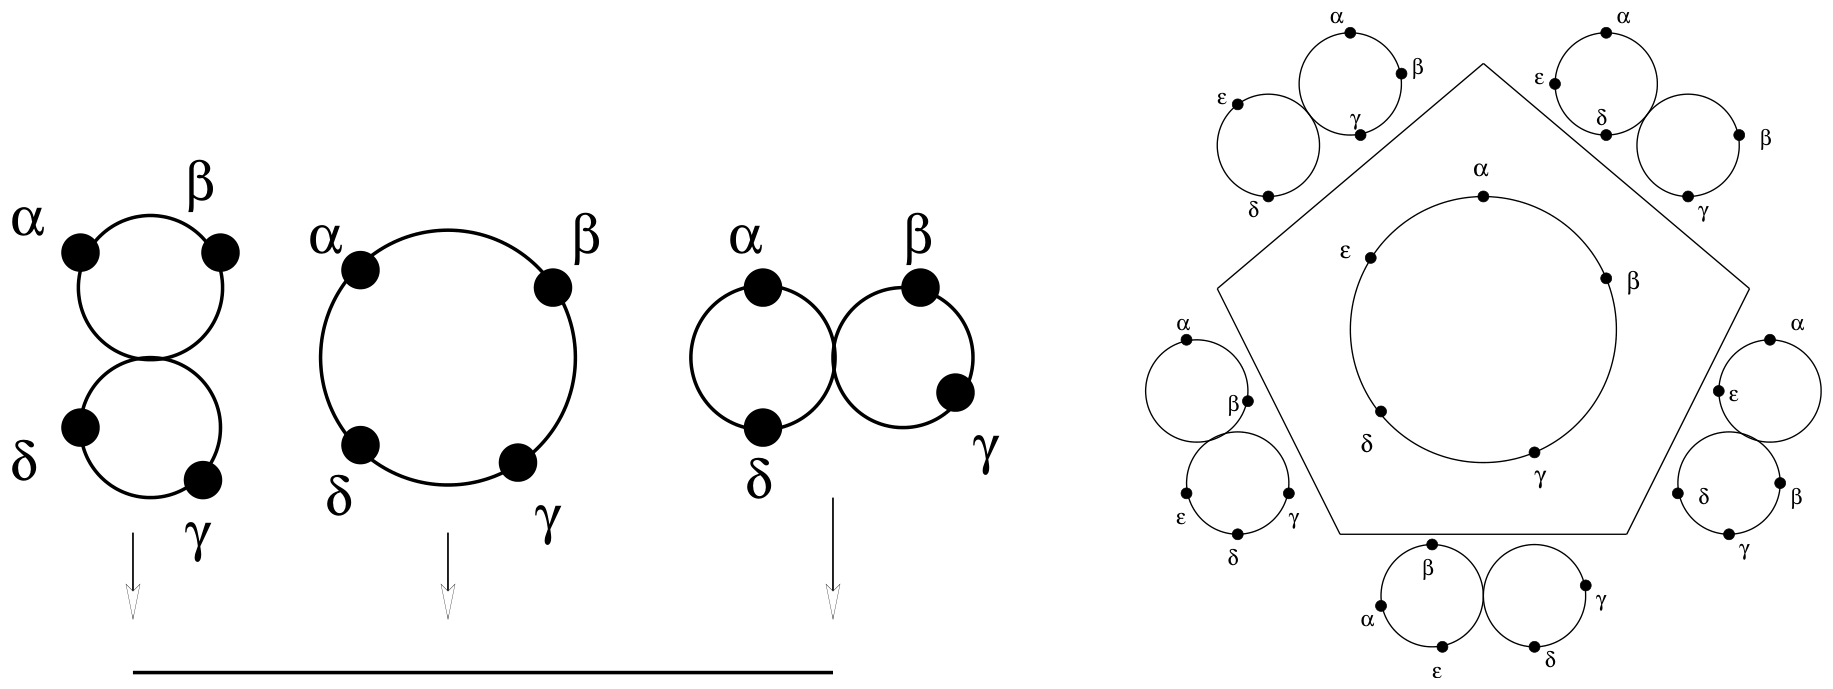
\includegraphics[width=0.95\textwidth]{fig10-dm-boundary.png}
  \caption{紧化 $\overline{\scrR}^4(\delta;\alpha,\beta,\gamma)$ 与 $\overline{\scrR}^5(\epsilon;\alpha,\beta,\gamma,\delta)$（原文 Figure~9，第 28 页）。\label{Fig:DMboundary}}
\end{figure}

\begin{Example} \label{Ex:CoveringSpace} Fukaya 范畴由全纯圆盘搭成，而全纯圆盘可以提升到覆叠空间。
设 $\pi:\tilde{M} \rightarrow M$ 是 Stein 流形的有限 Galois 覆叠，并以 $\scrF(\cdot)$ 记恰当 Fukaya 范畴。存在一个函子
$\pi^*: \scrF(M) \longrightarrow \scrF(\tilde{M})$，
它把 $L \in \scrF(M)$ 送到完全原像 $\pi^{-1}(L) \subset \tilde{M}$，并且态射上的映射 $HF^{*}(L,L) \to HF^{*}(\pi^{-1}(L), \pi^{-1}(L) )$
与经典的上同调拉回一致（由于群作用的不动点集假定为平凡，等变横截性不成问题）。$\pi$ 的覆叠变换通过 $\scrF(\tilde{M})$ 的自等价而作用。
\end{Example}

Fukaya 范畴是上同调幺的，因为 $HF^*(L,L)$ 是幺环。然而它们并非“几何地”严格幺，即通常不存在严格的单位元，除非施加某种抽象的拟同构。

% [Tutor Note: “上同调幺”与“几何严格幺”的区分值得留意：$[e_L]\in HF^*(L,L)$ 是幺元，但 $CF^*(L,L)$ 上通常没有严格单位元，必须先作抽象的拟同构才能得到严格幺模型；这正是 $A_\infty$ 范畴中“单位”只能在同伦意义下谈论的原因。]
在少数情形，可以把从扭曲复形 $\Tw\,\scrF(X)$ 到其幂等完备化 $\Tw^{\pi}\scrF(X)$ 的过渡理解如下：迭代的 Lagrange 手术（我们期望把它解释为映射锥）产生可能不连通的拉格朗日子流形，而取分裂闭包时就把各个连通分支都包括进来。一般并没有这样的几何解释：例如对于对角 $S^2 \subset \bP^1\times(\bP^1)^-$，Floer 上同调 $\cong QH^*(\bP^1)$ 有幂等元，而该对象的分裂项的同调类是 $(1\pm[S^2])/2$，并不落在纯次数上。

\subsection{扭转}

一类特别重要的映射锥来自扭转函子。给定 $Y \in$ Ob$\,\scrA$ 与一个 $\scrA$-模 $\scrM$，定义\emph{扭转} $\scrT_Y\scrM$ 为模
\[
\scrT_Y\scrM(X) = \scrM(Y)\otimes hom_{\scrA}(X,Y)[1] \oplus \scrM(X)
\]
它正是标准求值态射
\begin{equation} \label{Eqn:Twist}
\scrM(Y) \otimes \scrY \rightarrow \scrM,
\end{equation}
之上的锥，其中 $\scrY$ 表示 $Y$ 的 Yoneda 像。对两个对象 $Y_0, Y_1 \in$ Ob$\, \scrA$，扭转的本质特征是它在 $H(\scrA)$ 中给出一个标准的正合三角
\[
\cdots \rightarrow Hom_{H(\scrA)}(Y_0,Y_1) \otimes Y_0 \rightarrow Y_1 \rightarrow T_{Y_0}(Y_1) \stackrel{[1]}{\rightarrow} \cdots
\]
其中 $T_{Y_0}(Y_1)$ 是任一 Yoneda 像为 $\scrT_{Y_0}(\scrY_1)$ 的对象；若 $H(\scrA)$ 的态射空间有限维，这样的对象必然存在，参见 \cite[p. 64]{FCPLT}。
% [Tutor Note: 扭转公式 $\scrM(Y)\otimes hom(X,Y)[1]\oplus\scrM(X)$ 就是求值态射 $\scrM(Y)\otimes\scrY\to\scrM$ 的锥（$\scrY$ 的 Yoneda 像贡献出 $hom(X,Y)$）；因此“扭转 = 沿 Yoneda 模的锥”是 $A_\infty$-模层面的构造，而几何上的正 Dehn 扭转 $\tau_L$ 是 $\scrF(X)$ 的自等价——Seidel 定理断言二者在球面 $L$ 上拟同构，这把代数锥与 Lagrange 手术的映射锥对应起来。]

对 Fukaya 范畴，当 $L$ 为\emph{球面}的，即 $\Hom_{\mathrm{Don}(X)}(L,L) \cong H^*(S^n)$ 时，扭转函子 $\scrT_L \in nu$-$fun(\scrF(X),\scrF(X))$ 起着特殊的作用。设 $L\subset X$ 是拉格朗日球面；\emph{几何扭转} $\tau_L$ 是由 $L$ 中的正 Dehn 扭转所定义的 $\scrF(X)$ 的自等价，参见第~\ref{Sec:Appl1}~节。
另一方面，在单调或恰当情形，这样的球面给出 Fukaya 范畴 $\scrF(X)$ 的一个良好定义的对象（尽管在单调情形\emph{先验地}未必非零），从而给出上面所述的代数扭转函子。

\begin{Theorem}[Seidel] \label{Prop:twists}
若 $L\subset X$ 是拉格朗日球面，并在 $L \cong S^1$ 时带有非平凡的 \emph{Spin} 结构，则 $\tau_L$ 与 $\scrT_L$ 在 $nu$-$fun(\scrF(X),\scrF(X))$ 中拟同构。
\end{Theorem}
% [Tutor Note: 证明见 \cite[Corollary 17.17]{FCPLT}：其核心是把正 Dehn 扭转沿球面 $L$ 分解为“粘接”操作，再与 $HF^*(L,L)\cong H^*(S^n)$ 的代数数据逐项比对；注意 $L\cong S^1$ 时必须取非平凡 Spin 结构，否则定向线上差一个符号，结论会差一个平移。]

这就是 \cite[Corollary 17.17]{FCPLT} 在恰当辛流形情形下的结论，单调情形的论证类似。它给出了代数与几何之间的一个基本联系，并强化了我们此前在第~\ref{Subsec:ExactTriDon}~节中引入的 Donaldson 范畴中的正合三角。



%%%%%%%%%%%%%%%%%%%%%%%%%%%%%%%%%%%%%%%%%%%%%%%%%%%%%%%%%%%%%%%%%%%%%%%%%%%%%%%
%%  [Inlined] s04b-fukaya
%%%%%%%%%%%%%%%%%%%%%%%%%%%%%%%%%%%%%%%%%%%%%%%%%%%%%%%%%%%%%%%%%%%%%%%%%%%%%%%
% =============================================================================
%  s04b-fukaya.tex —— 第 4 节后半部分（§4.5--§4.8）
%  《A Symplectic Prolegomenon》(Ivan Smith, arXiv:1401.0269v2) 中文译注版
%  对应源码 p0269/src/Prolegomenon_utf8.tex 第 1165--1368 行
%  说明：本文件不含 \section 与 keypoints（节首由 s04a-fukaya.tex 负责），
%        直接从 §4.5 起排。
% =============================================================================

\subsection{分类策略}

理解给定辛流形 $(X,\omega)$ 的 Fukaya 范畴的一种策略包含三个基本步骤：选定一族“钟爱的”拉格朗日子流形 $\{L_i\}$；计算有限维代数 $\oplus_{i,j} HF^*(L_i, L_j)$ 上的 $A_{\infty}$-结构；然后证明 $\{L_i\}$（分裂）生成 $\scrF(X)$。核心的一步往往迂回进行，以尽量减少对 Cauchy--Riemann 方程显式解的需要。

\subsubsection{Hochschild 上同调}

$A_{\infty}$-范畴的 \emph{Hochschild 上同调}由如下的 bar 复形 $CC^*(\scrA,\scrA)$ 定义。次数为 $r$ 的上链是一个序列 $(h^d)_{d\geq 0}$，其中每一项是一族线性映射
\[
h^d_{(X_1,\ldots,X_{d+1})}: \bigotimes_{i=d}^1 hom_{\scrA}(X_i,X_{i+1}) \rightarrow hom_{\scrA}(X_1,X_{d+1})[r-d]
\]
对每个 $(X_1,\ldots,X_{d+1})\in \Ob(\scrA)^{d+1}$ 给出。微分由对拼接求和定义：
% [Tutor Note: $\maltese_i=\sum_{j=1}^i|a_j|-i$ 是定义 $A_\infty$ 关系时引入的 Koszul 符号（见第 2 节）。
%   Hochschild 微分的两项分别对应“在外层插入 $\mu$”与“先在内层插入 $\mu$”，符号 $(r+1)\maltese_i$ 与 $\maltese_i+r+1$ 极易记反；
%   核对办法是取 $d=2$ 的小情形逐项验证 $\partial^2=0$，并留意 $r$ 作为 $h$ 次数的整体移位始终保留在指数中。]
\begin{equation} \label{Eqn:Hochschild}
\begin{aligned}
(\partial h)^d & (a_d,\ldots, a_1) = \\
& \sum_{i+j<d+1} (-1)^{(r+1)\maltese_i} \mu_{\scrA}^{d+1-j}(a_d,\ldots,a_{i+j+1},h^j(a_{i+j},\ldots,a_{i+1}),a_{i},\ldots,a_1) \\
+ &  \sum_{i+j\leq d+1} (-1)^{\maltese_{i} +r +1}  h^{d+1-j} (a_d,\ldots,a_{i+j+1},\mu_{\scrA}^j(a_{i+j},\ldots,a_{i+1}),a_{i},\ldots,a_1).
\end{aligned}
\end{equation}
更简洁地说，事实上 $HH^*(\scrA,\scrA) = H(hom_{fun(\scrA,\scrA)}(\id,\id))$。域上 $A_{\infty}$-范畴的 Hochschild 上同调在取扭曲复形与幂等完备化之下均不变 \cite[Section 1c]{Seidel:Flux}。
% [Tutor Note: 把 $HH^*(\scrA,\scrA)$ 写成恒等函子的自同态复形的上同调，采用的是函子范畴中以 $\mu^1$ 为微分的标准约定；
%   它与 bar 复形的上同调同构，但具体上链的符号与次序约定可能相差一个符号，跨文献比较 $HH^*$ 的元素时必须先对齐约定。]

设 $A$ 是域 $\bK$ 上的 $\bZ_2$-分次代数，$\bK$ 的特征不等于 2。我们关心 $A$ 上微分平凡的那些 $\bZ_2$-分次 $A_{\infty}$-结构。这样的结构由一族映射
\[
\{ \alpha^i: A^{\otimes i} \rightarrow A \}_{i\geq 2}
\]
组成，其中 $\alpha^i$ 的奇偶性为 $i$。我们引入模 2 分次的 Hochschild 上链复形
\[
CC^{\bullet+1}(A,A) \ = \ \prod_{i \geq 2} Hom^{(\bullet+i)}(A^{\otimes i},A)
\]
其中 $Hom^{(\bullet +i)}$ 表示我们考虑奇偶性为 $\bullet+i$ 的同态。它带有通常的微分 $d_{CC^{\bullet}}$ 与 Gerstenhaber 括号 $[\cdot, \cdot]$。$A$ 上延拓其给定乘法的 $A_{\infty}$-结构 $(\alpha^i)$ 对应于满足 Maurer--Cartan 方程
\begin{equation} \label{Eqn:Maurer-Cartan}
d_{CC^{\bullet}} (\alpha) + \frac{1}{2} [\alpha, \alpha] = 0\qquad \textrm{with} \quad \alpha^1 = \alpha^2 = 0.
\end{equation}
的 $CC^{1}(A,A)$ 中元素 $\alpha$。
% [Tutor Note: 条件 $\alpha^1=\alpha^2=0$ 表示新的 $A_\infty$-结构保留原有乘法与零微分，只从 $\alpha^3$ 起才可能有非零项；
%   “规范变换”只在适当收敛条件下有效，实践中 $\bK$ 取 Novikov 域或 $\alpha$ 幂零时即可。]

$CC^0(A,A)$ 中的元素 $(g^i)_{i\geq 1}$（由奇偶性为 $i-1$ 的映射 $A^{\otimes i} \rightarrow A$ 组成）通过规范变换作用在 Maurer--Cartan 解集 $(\alpha^i)_{i\geq 2}$ 上，至少当适当的收敛性条件成立时如此。因此，给定代数 $A$ 上的 $A_{\infty}$-结构之集与 $A$ 的 Hochschild 上链复形紧密相联。为把这两种讨论联系起来：若 $\scrA$ 表示由 Maurer--Cartan 元素 $\alpha \in CC^1(A,A)$ 定义的 $A_{\infty}$-代数，且 $H(\scrA) = A$，则 $HH^*(\scrA,\scrA)$ 就是复形 $CC^{\bullet}(A,A)$ 关于扭微分 $d_{CC^{\bullet}} + [\cdot, \alpha]$ 的上同调。

由 \eqref{Eqn:ClosedOpen} 给出的闭-开弦映射 $\mathcal{CO}^0: QH^*(X) \rightarrow HF^*(L,L)$ 可以延拓为映射：只需考虑带有内部输入、若干边界输入以及单个边界输出的圆盘，
\begin{equation} \label{Eqn:COHH}
\mathcal{CO}: QH^*(X) \longrightarrow HH^*(\scrF(X), \scrF(X))
\end{equation}
我们仍称之为闭-开弦映射；将它与此前投影到 Hochschild 复形长度零部分的截断映射复合，就还原出先前引入的映射 \eqref{Eqn:ClosedOpen}。

\begin{Remark}\label{Rem:StarC1}
在 \ref{Subsec:ModuleStructures} 节中我们曾指出，Auroux、Kontsevich 与 Seidel 证明了：对单调辛流形，Fukaya 范畴 $\scrF(X)$ 可能的直和项被 $\ast c_1(X)$ 的特征值所指标。形式地，他们的论证始于如下观察：复合
\[
\mathcal{CO}^0: \ QH^*(X) \longrightarrow HH^*(\scrF(X), \scrF(X)) \longrightarrow HF^*(L,L)
\]
即 \eqref{Eqn:COHH} 与到 Hochschild 复形长度零部分的截断之复合，满足
\begin{equation} \label{Eqn:2c1degrees}
\mathcal{CO}^0(2c_1(X)) = 2 \frak{m}_0(L) \in HF^*(L,L).
\end{equation}
回忆在 $H^2(X,L) \rightarrow H^2(X)$ 下 $\mu_L \mapsto 2c_1(X)$，并取 Maslov 圈 $\mu_L \in H^2(X,L) = H^2_{ct}(X\backslash L)  \cong H_{2n-2}(X\backslash L)$ 的一个与 $L$ 不相交的代表 $D$，以消去常值圆盘的贡献，则 \eqref{Eqn:2c1degrees} 的两边本质上计数同一对象：一个边界落在 $L$ 上、内部标记点被约束在 $D$ 上的 Maslov 指标 2 圆盘。由指标原因，$\frak{m}_0(L) \in HF^*(L,L)$ 是单位元 $e_L$ 的倍数（同义反复地，若 $L$ 不界定任何 Maslov 指标 2 圆盘，则为零倍）。若 $\frak{m}_0(L) = \lambda e_L$，则
\[
QH^*(X) \rightarrow HF^*(L,L) \quad \mathrm{takes} \ 2(c_1-\lambda 1) \mapsto 0
\]
从而在特征 $\neq 2$ 时，$c_1-\lambda 1$ 不可逆。
\end{Remark}

\subsubsection{有限确定性\label{Subsec:FiniteDeterminacy}}

正如 Floer 上同调上的乘法在链层面有底层的 $A_{\infty}$-结构，Hochschild 上同调上的 Lie 括号在链层面有底层的 $L_{\infty}$-结构。Kontsevich 的形式性定理 \cite{Kontsevich:DefQuant} 断言：若 $A$ 是光滑交换代数，则在适当的滤过幂零条件下存在 $L_{\infty}$-代数的拟同构 $CC^*(A,A) \rightarrow HH^*(A,A)$，它在 Maurer--Cartan 解集上诱导双射。这使人能把 $A$ 上 $A_{\infty}$-结构的存在性与分类结果，转化为关于 Hochschild 上同调以及规范变换在其上作用的问题。

取 $A = \Lambda(V)$ 为有限维外代数可很好地说明这一结论。Hochschild--Kostant--Rosenberg 定理把 Hochschild 上同调等同于 $V$ 上多重向量场的 Lie 代数，即
\[
Sym^{\bullet}(V^{\vee}) \otimes \Lambda(V) \ = \ \bC[\![V]\!] \otimes \Lambda(V).
\]
其 Lie 代数结构来自 Schouten 括号
\begin{equation}
\begin{aligned} {}
& [f \,\xi_{i_1} \wedge \cdots \wedge \xi_{i_k}, g \,\xi_{j_1} \wedge \cdots \xi_{j_l}] = \\
& \textstyle \qquad \sum_q (-1)^{k-q-1} f \, (\partial_{i_q}g) \,
\xi_{i_1}  \wedge \cdots \wedge \widehat{\xi_{i_q}} \wedge \cdots
\wedge \xi_{i_k} \wedge \xi_{j_1} \wedge \cdots \wedge \xi_{j_l} + \\ & \textstyle \qquad
 \sum_q (-1)^{l-q+ (k-1)(l-1)} g \,(\partial_{j_q}f)\, \xi_{j_1} \wedge \cdots \wedge \widehat{\xi_{j_q}} \wedge \cdots \wedge \xi_{j_l} \wedge \xi_{i_1} \wedge
 \cdots \wedge \xi_{i_k}.
\end{aligned}
\end{equation}
由于 Schouten 括号在函数上为零，Kontsevich 定理蕴含：任何形式函数 $W\in\bC[\![V]\!]$ 定义一个 Maurer--Cartan 解，从而定义 $\Lambda(V)$ 上的一个 $A_{\infty}$-结构；并且相差一个形式微分同胚的拉回的两个函数，定义拟同构的 $A_{\infty}$-结构。

现设 $W$ 在 $0\in V$ 处有孤立临界点。于是奇点的经典有限确定性理论蕴含：$W$ 在形式坐标变换下等价于一个多项式。在这个意义上，由 $W$ 定义的 $A_{\infty}$-结构被有限量的数据完全决定（在拟同构意义下），从原则上说是可计算的，尽管 \emph{a priori} 它可能允许无穷多个非零乘积。有关一个概览性的例子见 \ref{Subsec:genus2} 节。
% [Tutor Note: 有限确定性保证 $W$ 经形式坐标变换可化为多项式，其次数 $d$ 给出上界：只有 $k\le d$ 时 $\mu^k$ 才可能非零，
%   因此尽管 $\mu$ 的指标集为无限，实际非零的乘积只有有限多个。“最高次非零 $\mu^k$”指 $k$ 最大的那个非零乘积，
%   它对应多项式最高次项经缩并所得的最后一层运算，其后再无更高阶乘积；不同多项式代表给出的结构在拟同构意义下相同。]

\subsection{生成\label{Sec:Generation}}

拥有一个判别有限族拉格朗日子流形生成 Fukaya 范畴的判据是重要的。具体地，给定 $L_1,\ldots,L_k \subset X$，有 $A_{\infty}$-代数
$\scrA \ = \ \oplus_{i,j} HF^*(L_i,L_j)$。
称 $L_i$ 分裂生成 $\scrF(X)$，若 $\scrF(X)$ 的每个对象都拟同构于 $\{L_i\}$ 上某个扭曲复形的一个直和项；这蕴含函子
\[
\scrF(X) \longrightarrow  \mathrm{mod}_{\!A_{\infty}}(\scrA), \qquad K \mapsto \oplus_i \, HF^*(K,L_i)
\]
是全忠实嵌入。我们将提到两个充分判据；后者更强，但前者在某些有趣的情形中适用。

\subsubsection{正关系}

先设 $\{L_1,\ldots, L_k\} \subset X$ 都是拉格朗日球面，并且满足一个 \emph{正关系}，即正 Dehn 扭转 $\tau_{L_i}$ 中的某个字 $w \in \langle \tau_{L_1}, \ldots, \tau_{L_k}\rangle$ 与恒等映射 Hamilton 同痕。字 $w$ 连同该同痕给出一个辛 Lefschetz 纤维化 $\scrX \rightarrow \bP^1$，其一般纤维辛同胚于 $X$，在 $\bC \subset \bP^1$ 上的单值性由 $w$ 给出，并经由给定的 Hamilton 同痕补全为 $\infty \in \bP^1$ 上的纤维化。坚持同痕是 Hamilton 的（而不只是辛的）之要点在于：$\scrX$ 的全空间此时带有延拓了来自 $X$ 的逐纤维结构的辛结构。特别地，$\scrX$ 中有良好的全纯曲线理论。

在陈述下述命题时，我们假设 $X$ 是单调的并在 $\bC$ 上工作，于是如注 \ref{Rem:StarC1} 那样，$\scrF(X) = \oplus_{\lambda} \scrF(X;\lambda)$，其中 $\lambda \in \mathrm{Spec}(\ast c_1(X))$。
% [Tutor Note: 正关系 $w\in\langle\tau_{L_i}\rangle$ 与恒等 Hamilton 同痕给出 $\scrX\to\bP^1$：$\bC$ 上的单值性为 $w$，$\infty$ 处由同痕补全。
%   圈类 $\mathcal{C}(w)\in QH^*(X)$ 的定义是“把 $\scrX\to\bP^1$ 的全纯截面在基点处取值”：截面族在纤维 $X$ 中扫出该圈。
%   它可视作 $w$ 所定义自等价在闭弦层面（量子上同调）的图形；“$\mathcal{C}(w)$ 幂零”刻画该自等价在相应直和项上的幂零性。]

\begin{Proposition} \label{Prop:SpheresGenerate}
令 $\mathcal{C}(w) \in QH^*(X)$ 表示把 $\scrX\rightarrow \bP^1$ 的全纯截面在某基点处取值所得的圈。设所有 $L_i$ 都属于 $\scrF(X; \lambda)$，且 $QH^*(X;\lambda) $ 上以 $\mathcal{C}(w)$ 作的量子上杯积是幂零的。则 $\{L_i\}$ 分裂生成 $\scrF(X;\lambda)$。特别地，若 $\lambda =0$ 且 $\mathcal{C}(w)$ 是 $c_1(X)$ 的倍数，则 $L_j$ 分裂生成 $\scrF(X;0)$。
\end{Proposition}

\begin{proof}
由代数 Dehn 扭转与几何 Dehn 扭转之间的对应（命题 \ref{Prop:twists}），存在正合三角
\[
\cdots \rightarrow  HF(L,K)\otimes L \rightarrow K \rightarrow \tau_L(K) \stackrel{[1]}{\longrightarrow} \cdots
\]
其中 $K \subset X$ 是范畴的 $\lambda$-直和项中的任意拉格朗日子流形。如 \eqref{Eqn:RollTriangle} 那样把 $w$ 中出现的 $\tau_{L_j}$ 对应的三角拼接起来，定义一个自然映射
\begin{equation}\label{eqn:concatenate}
K \rightarrow \prod_{i_j} \tau_{L_{i_j}} K \cong K
\end{equation}
它由 $HF^*(K,K)$ 的一个元素给出。从 Floer 上同调中长正合列的最初构造 \cite{Seidel:LES} 以及 \ref{Subsec:ExactTriDon} 节可知，自然映射 $K \rightarrow \tau_L(K)$ 来自计数一个环带上带单个临界点的 Lefschetz 纤维化的截面。粘合定理 \cite[Proposition 2.22]{Seidel:LES} 蕴含：这类映射的拼接计数了把若干这样的环带缝在一起所得的 Lefschetz 纤维化的全纯截面。在自然限制映射 $r: H^{*}(M) \rightarrow HF^{*}(K,K)$ 下，方程 \ref{eqn:concatenate} 由圈类 $r(\mathcal{C}(w)) \in HF^{*}(K,K)$ 的像作乘法给出。若 $\mathcal{C}(w)$ 消失，则迭代正合三角中的一个映射消失，于是 $K$ 是 $\{L_i\}$ 中若干对象的迭代锥的一个直和项。若 $\ast \mathcal{C}(w)$ 幂零，则把 $w$ 换成 $w^N$（$N \gg 0$）后可重复同一论证。
\end{proof}
% [Tutor Note: 证明中写作 $r: H^{*}(M)\to HF^{*}(K,K)$，但全文流形记为 $X$，$M$ 应为早期记号残留；
%   论证只用到限制映射的存在性与幺性，按 $r: H^{*}(X)\to HF^{*}(K,K)$ 理解即可。]

\subsubsection{Abouzaid 判据}

命题 \ref{Prop:SpheresGenerate} 的明显缺陷在于 $L_i$ 必须是球面。Abouzaid \cite{Abouzaid:generation} 在恰当情形给出了更好的判据，一般而言则由 Abouzaid--Fukaya--Oh--Ohta--Ono（准备中）给出；对单调流形，后者的解释见 \cite{RitterSmith, Sheridan3}。

\begin{Theorem}[Abouzaid-Fukaya-Oh-Ohta-Ono] \label{Thm:AFOOOgenerate}\label{Thm:Generation}
若映射 $\mathcal{CO}: QH^*(X) \rightarrow HH^*(\scrA,\scrA)$ 是同构，则 $L_i$ 分裂生成 $\scrF(X)$。
\end{Theorem}
% [Tutor Note: 判据的实质是“闭-开弦映射命中单位 $\Rightarrow$ 分裂生成”。$\mathcal{CO}$ 为同构时 $QH^*(X)$ 的单位映为 $HH^*$ 的单位，
%   而 $HH^*$ 的单位含于 $\{L_i\}$ 所生成的对象之中，故每个对象都是 $\{L_i\}$ 的扭曲复形的直和项。
%   注意 $\mathcal{CO}$（到 $HH^*(\scrA,\scrA)$）与 $\mathcal{CO}^0$（到 $HF^*(L,L)$）是不同层级的映射，切勿混用。]

考察定理 \ref{Thm:Generation} 所论情形的一个玩具模型是有启发性的：它只在 Hochschild 上同调的长度零部分层面运作，此时 \eqref{Eqn:COHH} 的闭-开弦映射约化为先前考虑过的较简单的 \eqref{Eqn:ClosedOpen}。设存在拉格朗日子流形 $L\in \scrF(X;\lambda)$，使得
\[
\mathcal{CO}^0: QH^*(X;\lambda) \rightarrow HF^*(L,L)
\]
是同构。我们将证明此时 $L$ 分裂生成 $\scrF(X;\lambda)$。事实上，对任意 $K\in \scrF(X;\lambda)$，只需证明映射
\begin{equation} \label{Eqn:HitUnit}
HF^*(L,K) \otimes HF^*(K,L) \longrightarrow HF^*(K,K)
\end{equation}
命中单位元 $1_K$。为验证这一点，在 \eqref{Eqn:HitUnit} 中写 $1_K = \sum_{j=1}^N p_j \cdot q_j$。存在映射
\[
\alpha = \sum_{j=1}^N \mu^2(p_j, \cdot) \quad \mathrm{and} \quad \beta = (\mu^2(q_1,\cdot),\ldots, \mu^2(q_N,\cdot))
\]
它们构成图表
\[
\xymatrix{
\bigoplus_{j=1}^N \, HF^*(L,L)\ar@<+2pt>@{->}^-{\alpha}[rr] \ar@<-2pt>@{<-}_-{\beta}[rr] && HF^*(L,K)
& \alpha \circ \beta  =1_K} 
\]
这表明 $\beta \circ \alpha$ 是幂等的，其像同构于 $HF^*(L,K) \subset \oplus_j HF^*(L,L)$ 的一个拷贝。由此，$K \in \Tw^{\pi}\langle L\rangle $ 是 $L$ 的若干拷贝的直和项（拟同构于幂等元 $\beta\circ\alpha$ 的像，而该像在取分裂闭包时被形式地作为一个对象引入）。
% [Tutor Note: 这里把“$L$ 分裂生成”化归为“乘法 (4.x) 的像含有 $1_K$”：一旦 $1_K\in \mathrm{im}(\mu^2)$，$K$ 就是 $L$ 的扭曲复形的直和项。
%   构造幂等元 $\beta\circ\alpha$ 时 $\alpha,\beta$ 的次序与转置极易颠倒：$\alpha$ 以 $p_j$ 为第一个变量，$\beta$ 以 $q_j$ 为第一个变量，
%   二者配对给出 $1_K$，反过来得到的 $\beta\circ\alpha$ 只是 $HF^*(L,K)$ 上的投影。]

\begin{figure}[ht]
  \centering
  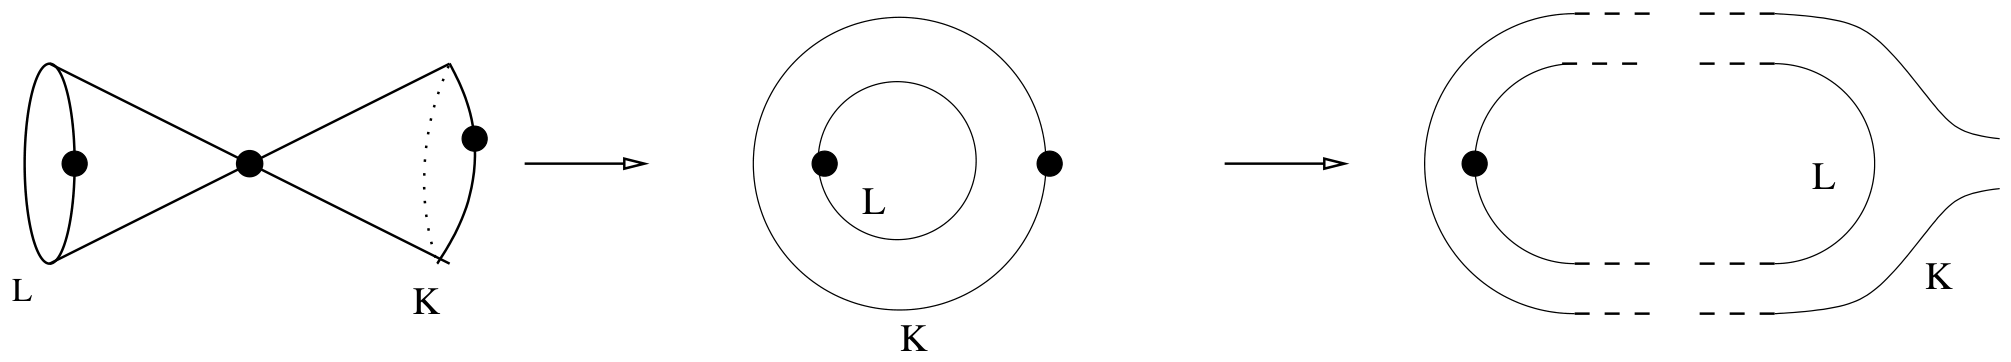
\includegraphics[width=0.85\textwidth]{fig11-cardy2.png}
  \caption{Cardy 关系的一个变体（原文 Figure~10，第 33 页）。\label{Fig:Cardy2}}
\end{figure}

为看出 \eqref{Eqn:HitUnit} 命中单位元，我们研究一参数族的环带，见图 \ref{Fig:Cardy2}（这类论证被称为 Cardy 关系，在此语境下可追溯到 \cite{BiranCornea}）。在该图左侧，我们在 $L$ 与 $K$ 的边界分支上固定标记点。把那个结点环带视为 $X\times X$ 中带原点处关联条件的圆盘，该图表示对角线的像
\begin{equation} \label{Eqn:Nodal}
\Delta \subset QH^*(X) \otimes QH^*(X) \longrightarrow HF^*(L,L) \otimes HF^*(K,K).
\end{equation}
若 tr$: HF^*(L,L) \cong QH^*(X;\lambda) \rightarrow \bC$ 是与基本类配对所给的 $QH^*(X)$ 上通常迹的限制，则我们因此得到一个类 $(\tr \otimes \id)(\Delta) \in HF^*(K,K)$。另一方面，图 \ref{Fig:Cardy2} 中间的环带（带有两个边界标记点）可沿一维退化的另一端分解为一条带一个边界标记点的条带与一个三穿孔圆盘。在此情形下，用 $HF^*(L,L)$ 上的迹封住该边界标记点，相当于考虑复合
\begin{equation} \label{Eqn:Smoothed}
\bK \rightarrow HF^*(L,K) \otimes HF^*(L,L) \otimes HF^*(K,L) \stackrel{\mathrm{tr}}{\longrightarrow} HF^*(L,K) \otimes HF^*(K,L) \stackrel{\mu^2}{\longrightarrow}HF^*(K,K). 
\end{equation}
通过这一参数族环带可以看出，$(\tr\otimes \id)(\Delta)$ 落在 \eqref{Eqn:Smoothed} 的像中，从而落在乘法 \eqref{Eqn:HitUnit} 的像中。由于对角线由 $[X]\otimes \id + $（其他项）给出，且 $QH^*(X) \rightarrow HF^*(K,K)$ 是幺的并透过 $QH^*(X;\lambda)$ 分解，比较 \eqref{Eqn:Nodal} 与 \eqref{Eqn:Smoothed} 即知 \eqref{Eqn:HitUnit} 的像包含单位元，正如所需。
% [Tutor Note: 对角类 $\Delta$ 的 Künneth 分解为 $[X]\otimes\id+$（其他项）：取 $\tr\otimes\id$（$\tr$ 为与基本类配对所得的迹）后，
%   $[X]\otimes\id$ 一项给出 $1_K$，而“其他项”经比较 (4.x) 与 (4.x) 可知已包含在乘法像中，这正是 (4.x) 命中单位的机制。
%   易错处：$QH^*$ 的分次移位与迹只取最高次分量的约定——按次数配对，低次项不进入单位。]

\subsection{应用 III}

我们继续贯穿全篇的主题：在一些典型情形中展示该代数机器；分别见 \cite{FSS,Nadler} 与 \cite{AbouzaidSmith:plumbing}。

\subsubsection{邻近拉格朗日\label{Sec:NearbyLag}}

余切丛的每个恰当拉格朗日子流形在 Fukaya 范畴中都同构于零截面，这是一个非平凡的定理，因此紧 Fukaya 范畴只含一个对象。该结果的证明经由对一个更有趣的范畴的描述，该范畴纳入非紧的拉格朗日子流形，即余切纤维。要点在于这些纤维生成 Fukaya 范畴（的适当版本）；这一事实已在 \eqref{Eqn:FibresShouldGenerate} 中初现端倪。

在技术层面有若干不同的途径，但任何一种都导致下述结果。设 $L\subset T^*Q$ 是 Maslov 类为零的恰当拉格朗日。Floer 上同调群 $HF^*(T^*_xQ,L)$ 构成 $Q$ 上一个 $\Z$-分次向量空间的平坦丛，记为 $E_L$。对 $L\subset T^*Q$ 可联系一个底层的链层面对象，即 $Q$ 上一个 $\bZ$-分次的 $dg$-层 $\scrE_L$，其纤维为 $CF^*(L, T_x^*Q)$；并论证这一对应把 Fukaya 范畴 $\scrF(T^*Q)$ 全忠实嵌入 $Q$ 上分次 $dg$-层构成的范畴。计算层 Ext 的通常局部-整体谱序列为
\[
E_1 = H^*(Q; \mathcal{E}xt(\scrE_L,\scrE_L)) \ \Longrightarrow \ \mathrm{Ext}^*(H(\scrE_L), H(\scrE_L))
\]
由 $\scrF(T^*Q)$ 嵌入的全忠实性，目标群可等同于 Floer 上同调 $HF^*(L,L)$。谱序列的 $E_2$-页于是给出
\begin{equation} \label{eq:ss}
E_2^{rs} = H^r(Q;\End^s(E_L)) \Rightarrow H^*(L;\bK)
\end{equation}
其中 $\End^*(E_L)$ 是分次自同态丛。由于 $\pi_1(Q)=0$，$E_L$ 是平凡丛，故 $E_2$ 页是一个“盒子” $H^*(Q) \otimes \End(HF^*(T^*_x,L))$。$E_2$ 层的微分从 $(r,s)$ 指向 $(r+2,s-1)$，更高页类似。于是盒子的左下角与右上角必定存活到 $E_\infty$。由于 $E_{\infty}$ 集中在次数 $0\leq \ast \leq n=\mathrm{dim}(Q)$，推出 $HF^*(T^*_x,L) \iso \bK$ 必须是一维的，且投影 $L \rightarrow Q$ 的度为 $1$。据此，谱序列退化，得 $H^*(L;\bK) \iso H^*(Q;\bK)$。还有另一个谱序列
\begin{equation} \label{eq:ss2}
E_1 = H^*(Q; \mathcal{E}xt(\scrE_Q,\scrE_L)) \ \Longrightarrow \ HF^*(Q,L).
\end{equation}
% [Tutor Note: 谱序列论证的关键是“盒子”形状：$E_2^{rs}=H^r(Q;\End^s(E_L))$ 的非零区域是 $0\le r\le n$ 且 $s$ 有界的矩形，
%   而收敛目标 $H^*(L;\bK)$ 只在 $0\le *\le n$ 非零，故矩形左下角与右上角必然存活到 $E_\infty$，迫使 $HF^*(T_x^*Q,L)$ 为一维。
%   其中用到 $\pi_1(Q)=0$ 使 $E_L$ 平凡；否则要把局部系数系统一并纳入，单值性会改变 $E_2$ 页。]

类似的分析表明边缘同态在最高次 $n$ 上是同构；该边缘同态可借助 Floer 乘积来解释，由此得出
\[
HF^n(T_x^*Q, L) \otimes HF^0(Q, T_x^*Q) \longrightarrow HF^n(Q,L) 
\] 
是同构，对任意 $x\in Q$ 成立。于是存在元素 $\alpha \in HF^0(Q,L)$，使得
\[
\mu^2(\alpha,\cdot): HF^*(T_x^*,Q) \rightarrow HF^*(T_x^*,L)
\]
是同构；但由于纤维生成该范畴，这恰好说明 $\alpha$ 在 $\scrF(T^*Q)$ 中定义了 $Q$ 与 $L$ 之间的同构。
% [Tutor Note: 原文此处写 $HF^*(T_x^*,Q)$ 与 $HF^*(T_x^*,L)$，按上下文应为 $HF^*(T_x^*Q,Q)$ 与 $HF^*(T_x^*Q,L)$（$x\in Q$ 为基点）。
%   此处照抄原文以求保真，请勿径改。]

\subsubsection{映射类群\label{Sec:MCGIII}}

定理 \ref{Prop:twists} 的一部分是如下陈述：对任意对象 $L \in \scrF(X)$ 都存在的代数扭转函子 $T_L$，当 $L$ 是球面时可逆。该论证可纯粹代数地给出，并且当 $L=\Sigma$ 是任意整系数同调球面时同样适用。令 $M_{\Sigma} = T^*\Sigma\#T^*S^n$ 为把给定的余切丛作管道连接（plumbing）所得的流形，即把一个 $T^*\Sigma$ 的纤维封顶成一个闭拉格朗日球面（该手术可在 Stein 范畴中实施）。$\bZ_2$-分次的恰当 Fukaya 范畴 $\scrF(M_{\Sigma})$ 容许自函子 $T_{\Sigma}$，由于 $\Sigma$ 是同调球面，它是等价。容易看出该等价是无穷阶的。设 $\pi_1(\Sigma)$ 有限但非平凡。我们断言 $T_{\Sigma}$ \emph{不是}由任何紧支辛同胚诱导的，即 \emph{不存在几何 Dehn 扭转}。（我们引入 $M_\Sigma$ 是为了给出一个完全用闭拉格朗日、而不用非紧余切纤维的论证。）

令 $\iota: \tilde{\Sigma} \rightarrow \Sigma$ 表示万有覆叠，$\pi: \tilde{M}_{\Sigma} \rightarrow M_{\Sigma}$ 为诱导的覆叠。固定一个特征整除 $\iota$ 的指数的系数域 $\bK$。反设代数扭转 $T_{\Sigma}$ 由某个紧支辛同胚 $\tau$ 诱导。考察 $\tau \circ \tau$ 或其逆，并回忆方程 \ref{Eqn:Twist} 中扭转函子的定义，我们推断存在一个恰当拉格朗日子流形 $L \subset M_{\Sigma}$，它表示扭曲复形
\begin{equation} \label{Eqn:ImpossibleComplex}
\Sigma \leftarrow \Sigma \leftarrow S^n
\end{equation}
其中最左的箭头由乘以基本类 $[\Sigma]$ 给出，$S^n$ 是另一个核心分支。现在回忆例 \ref{Ex:CoveringSpace}。\eqref{Eqn:ImpossibleComplex} 在 $\scrF(\tilde{M}_{\Sigma})$ 中的原像由 $\tilde{\Sigma} \leftarrow \tilde{\Sigma} \leftarrow \pi^{-1}(S^n)$ 表示，其中\emph{左微分消失}：它由 $\Sigma$ 的基本类拉回得到，故按我们对 $\bK$ 的特征的选取，它在系数域 $\bK$ 中为零。

作为连通拉格朗日子流形 $L$ 在一个覆叠下的原像，$\pi^{-1}(L)$ 的所有分支都微分同胚，并且由覆叠变换相联系，从而是 $\scrF(\tilde{M}_{\Sigma})$ 的自等价。复形 $\Sigma \leftarrow S^n$ 是 $\Sigma$ 在 $S^n$ 中 Dehn 扭转下的像。因此，$\tilde{\Sigma}$ 与 $\tilde{\Sigma} \leftarrow \pi^{-1}(S^n)$ 都由连通拉格朗日表示，从而都是不可分解对象（我们在 $\bZ$-分次情形，且对连通拉格朗日 $HF^0$ 的秩为 $1$）。同样由例 \ref{Ex:CoveringSpace}，它们不在覆叠变换的同一轨道中：取与 $  \pi^{-1}(S^n)$ 的某个分支处的余切纤维作 Floer 上同调，Floer 群在一种情形秩为 $0$，在另一种情形秩为 $1$。上一段表明，在相差平移的意义下，
\begin{equation} \label{Eqn:SplitPreimage}
\pi^{-1}(L) \cong \tilde{\Sigma} \oplus \left( \tilde{\Sigma} \leftarrow \pi^{-1}(S^n) \right)
\end{equation}
在范畴 $\scrF(\tilde{M}_{\Sigma})$ 中成立。我们现已证明 \eqref{Eqn:SplitPreimage} 的右端不同构于单个覆叠群轨道内的不可分解对象之直和，这是矛盾。
% [Tutor Note: 论证骨架：若 $T_\Sigma$ 有几何实现，则 (4.x) 的扭曲复形由某个恰当拉格朗日 $L$ 表示；
%   覆叠后最左微分由 $[\Sigma]$ 拉回、按特征选取在 $\bK$ 中为零，于是 $\pi^{-1}(L)$ 分裂成两个不可分解对象之直和，而二者分属不同覆叠轨道，矛盾。
%   易错点：$\tau$ 与 $\tau^{-1}$ 对应的扭曲复形相差一次平移，会改变 $[\Sigma]$ 前的符号；选取 $\tau\circ\tau$ 正是为了消除这一歧义。]

\begin{Notes} 关于 $A_{\infty}$-代数与 Fukaya 范畴的背景，见 \cite{FCPLT, FO3}。关于 Hochschild 上同调与形变理论的论证，见 \cite{Seidel:HMSquartic, Seidel:HMSgenus2}。
\end{Notes}



%%%%%%%%%%%%%%%%%%%%%%%%%%%%%%%%%%%%%%%%%%%%%%%%%%%%%%%%%%%%%%%%%%%%%%%%%%%%%%%
%%  [Inlined] s05-examples
%%%%%%%%%%%%%%%%%%%%%%%%%%%%%%%%%%%%%%%%%%%%%%%%%%%%%%%%%%%%%%%%%%%%%%%%%%%%%%%
% ============================================================================
%  s05-examples.tex —— 第 5 节「例子」
%  原文：Ivan Smith, A Symplectic Prolegomenon, arXiv:1401.0269v2
%  对应源码：p0269/src/Prolegomenon_utf8.tex 第 1369--1494 行
% ============================================================================

\section{例子}\label{Sec:Examples}

\begin{keypoints}
\begin{itemize}
  \item \textbf{核心图像}：本节以一批可以“显式”计算的流形，说明 Fukaya 范畴的生成元与显式代数模型：二维环面、亏格 2 曲面、四维环面、偶维二次超曲面、环簇 Fano 簇与四次 K3 曲面。
  \item \textbf{关键工具}：球状对象的生成判据（命题 \ref{Prop:SpheresGenerate}）、Lefschetz 纤维化与扭曲复形、道路代数的 $A_{\infty}$-结构、quilt 型 Künneth 定理、pearl 模型与谱序列。
  \item \textbf{结论}：这些例子的导出 Fukaya 范畴分别等价于椭圆曲线上的凝聚层、$E\times E$ 上的凝聚层、显式 $A_{\infty}$-代数上的模等代数对象；反过来，范畴计算也给出辛拓扑结论（例如四维环面上辛同胚的不动点下界）。
  \item \textbf{与前后文的联系}：本节把前文的生成判据与 $A_\infty$ 代数工具落到实处，并为第 6 节的稳定性条件与 Orlov 谱提供计算素材。
\end{itemize}
\end{keypoints}

我们“显式地”描述若干流形的 Fukaya 范畴。这些例子是实曲面（其上的拉格朗日圆圈不界定任何圆盘）、Calabi--Yau 曲面（由例 \ref{Ex:CY} 所支配）或单调簇，因此这些范畴可以用初等手段定义。

\subsection{二维环面} 取 $\bK = \Lambda$。应用命题 \ref{Prop:SpheresGenerate} 可知，经圈 $l$ 与子午圈 $m$ 分裂生成 $\scrF(T^2)$。事实上，$(\tau_l \tau_m)^6 = \id$，相应的 Lefschetz 纤维化 $\scrX \rightarrow \bP^1$ 是有理椭圆曲面，而圈类 $\mathcal{C}(w)$ 计数有限多条 $(-1)$-曲线截面，故其取值是 $H^2(T^2)$ 中最高类的非零倍数。圆圈 $l$、$m$ 不界定任何全纯圆盘，故其自 Floer 上同调等于 $H^*(S^1)$。两圆横截相交于唯一一点，这给出生成元 $[p]\in HF^0(l,m)$ 与 $[q]\in HF^1(m,l)$。这里 $p$ 的分次是选定的，而 $q$ 的分次由 Poincaré 对偶强制决定；后者同时蕴含乘积 $\mu^2(p,q)$ 与 $\mu^2(q,p)$ 非平凡。由分次理由，除幺性所强制的乘积之外，这些就是全部非平凡乘积。

% [Tutor Note: $(\tau_l\tau_m)^6=\id$ 即椭圆纤维化的辫关系，是模群 $SL(2,\bZ)$ 中“双曲”元素的阶；它是把 $T^2$ 的 Lefschetz 纤维化实现为有理椭圆曲面的关键。核对时注意 $\tau_l,\tau_m$ 为沿 $l,m$ 的正 Dehn 扭转，方向或符号约定相反时会得到 $(\tau_l\tau_m)^{-6}$，但不影响本段论证。]

由此可知，六维代数 $A = HF(l \oplus m, l \oplus m)$ 可以描述为下图箭图 $Q$ 的道路代数 $\Pi\,Q$ 的商
\begin{equation*}
\xymatrix{
 l \ \ar@/^/^{[p]}[r] & \ m\ar@/^/^{[q]}[l]
}
\end{equation*}
模去由合成 $a\rightarrow b\rightarrow a \rightarrow b$ 与 $b\rightarrow a \rightarrow b \rightarrow a$ 生成的理想，亦即 $\Pi\,Q / \langle J\rangle^3$，其中 $J$ 为所有箭头生成的理想。对于道路代数模去箭头理想的幂所得的商，bar 复形含有大量零调子复形，这意味着 Hochschild 上同调可以相当容易地计算。

从这里出发，Lekili 与 Perutz \cite{LekiliPerutz} 确定了六维代数 $A$ 上所有可能的 $A_{\infty}$-结构。

% [Tutor Note: 作者说“bar 复形含大量零调子复形”而未给证明；其要点是：模去箭头理想的高次幂后，商代数在道路长度滤过下的各项是半单的，于是 Hochschild 链复形可按滤过逐层用标准的条复形（bar/Koszul）论证消去。具体计算建议先分别处理 $J^2$ 与 $J^3$ 两层，再核对乘法 $\mu^2$ 的复合是否恰落入 $\langle J\rangle^3$。]

\begin{Theorem}[Lekili--Perutz]\label{Thm:LPelliptic}
设 char$(\bK) \not\in \{2,3\}$。$A$ 上的任意极小 $A_{\infty}$-结构都规范等价于如下子范畴：在三次曲线族
\[
\{y^2z = 4x^3 - pxz^2 - qz^3 \} \subset \mathbb{A}^2_{p,q}  \times \bP^2
\]
中唯一一条三次曲线上，层的导出范畴里由结构层 $\mathcal{O}$ 与摩天层 $\mathcal{S}_{[0,1,0]}$ 生成的子范畴。
\end{Theorem}

Lekili 与 Perutz 还证明，若在判别式 $\{p^3 = 27 q^2\}$ 上取一点（此时三次曲线出现结点），则该范畴重现 $\scrF(T^2 \backslash \{pt\})$ 中由 $\{l,m\} \subset T^2\backslash \{pt\}$ 生成的子范畴；这尤其表明后者不是形式（formal）的——尽管去一点的二维环面是恰当的，唯一的非平凡全纯多边形是常值多边形（关键在于，这些常值多边形并非横截地切出，因此必须“虚拟地”计数）。这说明了在不借助代数分类结果的情况下，直接对 Fukaya 范畴作计算之困难。

\subsection{亏格 2 曲面\label{Subsec:genus2}} 考虑以原点与五次单位根为分支点的超椭圆曲线 $\Sigma_2 \rightarrow \bP^1$。取定 $\omega_{\Sigma_2}$ 拉回到 $T\Sigma_2$ 的单位圆丛上的一个原语（primitive）$\theta$。虽然 $\Sigma_2$ 不是单调的，它仍有定义良好的“平衡”Fukaya 范畴（在 $\bC$ 上线性），其对象是满足 $\int_{\gamma} (D\gamma)^*\theta = 0$ 的拉格朗日圆圈 $\gamma: S^1 \hookrightarrow \Sigma_2$。（曲线的非可缩同痕类含有唯一的平衡代表元；对以平衡边界条件为界的多边形，能量与指标是相关的；最后，范畴 $\scrF(\Sigma_2)$ 在拟同构意义下与 $\theta$ 的选取无关。）一族 $5$ 条平衡曲线 $\gamma_i$ 由图 \ref{Fig:BalancedSphere} 左侧所示的匹配路径给出，且由命题 \ref{Prop:SpheresGenerate} 的又一次应用，它们分裂生成该 Fukaya 范畴。

% [Tutor Note: 本段括号中“能量与指标相关”一句是平衡 Fukaya 范畴的命脉：平衡条件 $\int_\gamma (D\gamma)^*\theta=0$ 保证全纯多边形的 Maslov 指标与其辛面积成固定比例，从而可用能量（等价地，指标）作 $\bZ$-分次并定义定向；若丢掉该条件，范畴只剩 $\bZ_2$-分次，$\mu^k$ 的符号与次数都会失去意义。核对时切勿把这里的“balanced”与单调（monotone）混为一谈。]

\begin{figure}[ht]
  \centering
  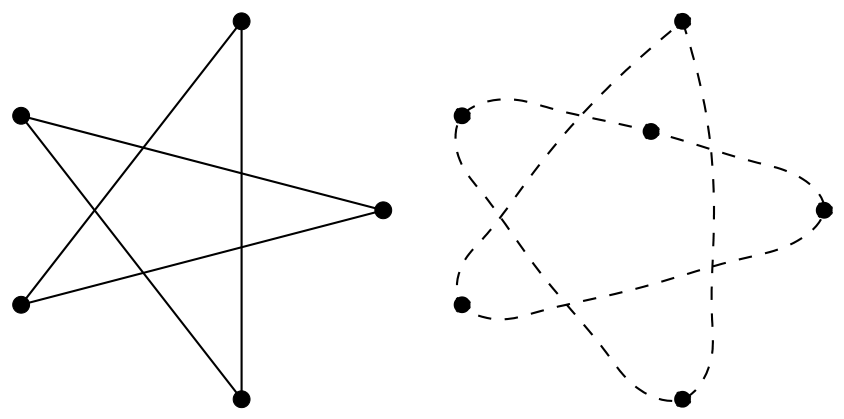
\includegraphics[width=0.5\textwidth]{fig12-pentagram.png}
  \caption{$\scrF(\Sigma_2)$ 的生成元与一个全纯六边形（原文 Figure~11，第 37 页）。\label{Fig:BalancedSphere}}
\end{figure}

选择 $\gamma_i$ 作为分裂生成元的动机来自 Seidel 的观察 \cite{Seidel:HMSgenus2}：
\[
\oplus_{i,j} HF^*(\gamma_i, \gamma_j) \ \cong \ \Lambda^*(V) \rtimes \bZ_{5}
\]
其中 $V$ 是三维向量空间。于是 $A_{\infty}$-结构可以借助第 \ref{Subsec:FiniteDeterminacy} 节的工具来处理（在存在有限群作用的情形下，这些工具有直接的等变版本），即以多向量场（polyvector field）来描述。直接计算表明，$A_{\infty}$-结构由一对 $(W,\eta)$ 给出，其中包含一个形式函数与一个形式 2-形式，满足
\[
W=z_1z_2z_3 + z_1^{5} + z_2^{5} + z_3^{5} + O(6)
\]
（我们忽略符号，它们可以通过在 Floer 复形中作适当的基变换来调整）。低阶非平凡系数来自高阶乘法 $\mu^3$ 与 $\mu^5$，它们由“明显”的全纯多边形确定：位于五角星各角处的三角形，或如图 \ref{Fig:BalancedSphere} 右侧所勾画边界的五边形（其到 $\bP^1$ 的投影在内五边形上以重数二覆盖）。在每种情形中，这些多边形都有一个额外的边界标记点，映射在该点处光滑但被限制在给定的某个拉格朗日上的一个圈上；在相应的四边形、六边形中，这表现为两条相邻的边界条件。由于 $W$ 在 $0$ 处有孤立奇点，它经形式变量替换等价于一个多项式，且事实上等价于其 $\leq 5$ 次 Taylor 级数。这以显式 $A_{\infty}$-代数上的模完整描述了 $\scrF(\Sigma_2)$ 的分裂闭包。

\subsection{四维环面\label{Sec:4torus}} 取 $\bK = \Lambda$。定理 \ref{Thm:LPelliptic} 的一个特殊情形（它更早即已为人所知）表明 $D^{\pi}\scrF(T^2) \simeq D^b(E)$，其中 $T^2$ 是方形辛环面，$E$ 是 Tate 曲线。Fukaya 范畴服从某种 Künneth 定理 \cite{AbouzaidSmith}；利用 Wehrheim--Woodward quilt 理论（的 $A_{\infty}$-精细版本），即第 \ref{Sec:Quilt} 节与 \eqref{Eqn:QuiltFunctor}，可以把 $D^{\pi}\scrF(T^2 \times T^2)$ 等同于 $D^{\pi}\scrF(T^2) \simeq D^b(E)$ 的自函子范畴。由此可知 $\scrF(T^4)$ 由四个拉格朗日二维环面 $l\times l, l\times m, m\times l, m\times m$ 分裂生成，且
\begin{equation} \label{Eqn:HMST4}
D^{\pi} \scrF(T^4) \simeq D^b(E\times E).
\end{equation}
\eqref{Eqn:HMST4} 对四维环面的辛拓扑有具体推论。设 $\phi: T^4 \rightarrow T^4$ 是一个在上同调上平凡作用的辛同胚。则它有定义良好的通量（flux），即：对任意 1-圈 $\gamma \in H_1(T^4)$，可取 2-链 $C_{\gamma}$ 使 $\partial C_{\gamma} = \gamma \cup \phi(\gamma)$，并考虑 $\int_{C_{\gamma}} \omega \in \bR / \bZ$，其中模去辛形式的周期便消除了 $C_{\gamma}$ 选取的不唯一性。

% [Tutor Note: Tate 曲线 $E$ 是 Novikov 域上的一条椭圆曲线，$D^{\pi}\scrF(T^2) \simeq D^b(E)$ 正是二维环面同调镜像对称的精确化。注意“方形”条件并非多余：$T^2$ 的辛面积与复结构参数决定 $E$ 的模参数（$j$-不变量），改变 $T^2$ 的复结构会改变镜像曲线。另一个易混点：通量是辛同胚同痕类的“平移部分”，Hamilton 同胚的通量恒为零。]

\begin{Proposition} 若 $\phi$ 的通量为零，则 $\phi$ 的 Hamilton 同痕类中任何具有非退化不动点的辛同胚都至少有 $16$ 个不动点。\end{Proposition}

\begin{proof}
$D^b(E\times E)$ 的自等价通过 Mukai、Orlov 与 Polishchuk 的工作已被完全理解，见 \cite{Orlov:abelian, Pol:weil}；那些在上同调上平凡作用的自等价，模去平移（shift），由张量以线丛以及 $E\times E$ 的平移生成。在辛侧，这些分别对应两类自等价：平移 $T^4$（具有非零通量），或给拉格朗日配备非平凡的局部系数（后者在空间层面、即 $T^4$ 的点上平凡作用）。因此，$\phi$ 与 $\scrF(T^4)$ 的恒等自等价（或 $T^4$ 的恒等辛同胚）有相同的 Floer 上同调，而后者恰为 $H^*(T^4)$。
\end{proof}

\subsection{二次超曲面}\label{Sec:Quadrics}

设 $X=Q \subset \bP^{2k+1}$ 为偶维二次超曲面。任何二次超曲面至多有一个结点，故 $X$ 含有一个在等痕意义下典范的拉格朗日球面 $L$：它是某个代数退化的消没圈，且这样的球面唯一。当 $k>0$ 时，它的极小 Maslov 数为 $2c_1(Q) > 2$，故落在零和分支 $\scrF(Q;0)\subset \scrF(Q)$ 中。

\begin{enumerate}
\item 设 $\scrX \rightarrow \bP^1$ 为二次超曲面族的一个 Lefschetz 铅笔的全空间：所有消没圈都同痕于固定的拉格朗日 $L$。容易验证，唯一的全纯截面来自对该铅笔底轨迹的爆破，因而在单个纤维中取值于 $Q \cap Q' \subset Q$，与第一 Chern 类成比例。于是命题 \ref{Prop:SpheresGenerate} 适用，$L$ 分裂生成 $\scrF(Q;0)$。
\item 或者考虑映射 $QH^*(Q;0) \rightarrow HF^*(L,L)$。两个空间秩均为 $2$，映射是幺的，故在 $0$ 次非平凡；又因 $[L] \neq 0 \in H_{2k}(Q)$，映射在 $2k$ 次非平凡（两边均按模 $4k$ 分次），故生成判据的第二个版本也适用。
\end{enumerate}

代数 $HF^*(L,L)$ 是半单的。由 $L$ 生成蕴含 $D^{\pi}\scrF(Q;0)$ 本质上是平凡的（等价于两个域上模之和，即向量空间对），见 \cite{Smith:HFQuadrics}。任何单连通的拉格朗日 $K \subset Q$ 都定义这样一个模，其自同态代数一方面是 $HF^*(K,K)$，另一方面是两个矩阵代数之和。

由于 $N_{min}(K) = 4k$，命题 \ref{Lem:Oh} 的 pearl 模型表明 Oh 谱序列按分次理由坍塌，且加性地有 $HF^*(K,K) \cong H^*(K)$。一个相当简单的代数几何计算 \cite{Beauville} 表明，量子上同调 $QH^*(Q)$ 含有一个 $2k$ 次的可逆元 $a$。由于 $\mathcal{CO}^0$ 是幺环同态，与 $\mathcal{CO}^0(a)$ 作积定义了（$\bZ/4k$-分次群）$HF^*(K,K)$ 的一个自同构；按命题 \ref{Lem:Oh} 的证明中提到的乘法 pearl 模型，该自同构由与 $a|_K$ 的经典杯积以及次数 $\leq 2k-N_{min}(K) = -2k$ 的修正给出。由此可知 $H^*(K)$ 在次数 $0<\ast< 2k$ 上消失，故 $K$ 是同调球面。又因 $H^*(K)$ 是两个矩阵代数之和，它必是两个一维如此代数之和，故 $K$ 定义的模与 $L$ 相同。于是 $K$ 在 $\scrF(Q;0)$ 中同构于 $L$，从而 $K \cap L \neq \emptyset$；特别地，任意两个单连通拉格朗日都不能经 Hamilton 同痕彼此移开。

% [Tutor Note: 这一段分次极易错位：$Q\subset\bP^{2k+1}$ 的复维数是 $2k$，$HF^*$ 是模 $4k$ 分次的（分次周期来自 $2c_1(Q)$），而 $QH^*$ 也是模 $4k$ 分次。文中“$[L]\neq 0\in H_{2k}$ 故映射在 $2k$ 次非平凡”依赖两侧分次约定的对齐；若套用通常的 $\bZ$-分次，$2k$ 会被误认为 $k$。]

任意 $Q$ 的辛同胚在 $\Auteq(\scrF(Q;0)) \cong \bZ_2$ 中都与恒等或与 Dehn 扭转 $\tau_L$ 重合，后者交换 $HF^*(L,L)$ 的两个幂等分支。由于二次曲面的粗模空间 $\EuScript{Q}$ 有基本群 $\bZ_2$，这意味着问题 \ref{Question:Monodromy} 中的映射在此情形是单射。

\subsection{环簇 Fano 簇} 设 $X$ 是环簇 Fano 簇，矩映射为 $\mu: X \rightarrow \frak{t}^*$，矩像为 $\Delta$。以矩映射的纤维为边界的 Maslov 2 圆盘由矩多面体 $\Delta$ 的余维一的面（facets）逐一枚举，这些计数可以组装成一个 Laurent 多项式 $W: \mathrm{int}(\Delta) \rightarrow \Lambda$，其单项式项由 $\Delta$ 各面的法向量决定，见 \cite{Cho,Cho-Oh}。（这个记号反映了如下事实：它契合第 \ref{Sec:Mirror} 节顺带提到的势函数一般图景。除子 $D$ 是 $X$ 的环簇边界，矩映射给出 $X\backslash D$ 的拉格朗日纤维化，而镜像 $\Cech{U} \cong (\bC^*)^n$。对 $\bP^2$，$W(x,y) = x+y+\lambda/xy$。）例 \ref{Ex:ToricFibre} 蕴含：矩映射的给定纤维的 Floer 上同调在某个局部系数下非平凡（即 $\partial_1 = 0$），当且仅当矩多面体的相应点是 $W$ 的临界值。

% [Tutor Note: 请牢牢记住“矩多面体的余维一面 $\leftrightarrow$ Maslov 2 圆盘类”这部字典：每个面贡献一个以矩映射纤维为边界的圆盘类，其（虚拟）计数给出 $W$ 中相应单项式的系数；而 $W$ 的临界点正对应那些可配上局部系数使 $\partial_1=0$ 的纤维（例 \ref{Ex:ToricFibre}）。这正是环簇镜像对称中 Landau--Ginzburg 势的辛侧来源。]

设 $X$ 的复维数为偶数 $n=2k$，且量子积 $\ast c_1(X)$ 的谱是单的，于是 $QH^*(X) = \oplus_{\lambda} QH^*(X;\lambda)$ 分解为域之和。此时存在 $\mathrm{rk}(QH^*(X))$ 个不同的局部系数 $\xi_j \rightarrow L$，定义在重心 $b\in\Delta$ 上方的环簇纤维 $L$ 上，使得 $HF^*(\xi_j, \xi_j)$ 非零；事实上在每种情形它都是 Clifford 代数（参见 \cite{Cho-Oh, FO3:toric, RitterSmith}）。对象 $(\xi_j \rightarrow L)$ 分裂为两两同构（至平移）的幂等元之和；偶维 Clifford 代数是矩阵代数，而闭-开弦映射
\[
QH^*(X;\lambda_j) \longrightarrow \bK \subset HH^*(Cl_n, Cl_n) 
\]
是到任一给定幂等分支的自同态子代数上的同构，因为该映射是幺的且两侧秩均为 1。定理 \ref{Thm:Generation} 蕴含 Fukaya 范畴由 $(L,\xi_j)$ 分裂生成，因此任何满足 $HF(K,K)\neq 0$ 的拉格朗日 $K$ 必与 $\mu^{-1}(b)$ 相交。

\subsection{四次曲面\label{Sec:K3}} 设 $Q= \{z_0^4+\cdots + z_3^4 = 0\}$ 为四次 $K3$ 曲面。由
\begin{equation}\label{pencil}
\lambda(z_0^4+ \cdots z_3^4) + z_0z_1z_2z_3
\end{equation}
定义的四次曲线铅笔在 $\lambda = 0$ 处的纤维之外是 Lefschetz 的，而 $\lambda = 0$ 处的纤维是坐标超平面之并。该铅笔有 $64$ 个结点纤维，由此得到 $Q$ 中一族 $64$ 个拉格朗日球面 $V_i$。以这些球面作正 Dehn 扭转的词通过一个平移作用在 $\scrF(Q)$ 上 \cite{Seidel:HMSquartic}；由命题 \ref{Prop:SpheresGenerate} 的一个变体可知这些球面分裂生成（此时 \eqref{eqn:concatenate} 中的映射因分次理由为零）。利用情形的对称性，Seidel 证明了
\[
\scrA(Q) \, = \, \oplus_{i,j} HF^*(V_i, V_j) \, \cong \, \Lambda(W) \rtimes \Gamma_{64}
\]
其中 $W$ 是四维复向量空间，$\Gamma_{64} \subset H \subset SL(W)$ 是 $SL(W)$ 的极大环面 $H$ 中由阶为 $4$ 的元素构成的有限子群。Hochschild 上同调 $HH^*(\Lambda(W)\rtimes \Gamma_{64})$ 含有由等变多向量场构成的和分支 $HH^*(\Lambda(W))^{\Gamma_{64}}$。对应于非弯曲形变（此时拉格朗日保持无障碍）的子群在 $2$ 次秩为 $7$，且存在\emph{唯一}一个在 $GL(W)$ 的 $\bZ_4$-子群（循环置换各坐标）下不变的类。该对称性保持铅笔 \eqref{pencil}，且 $\scrF(Q)$ 上的 $A_{\infty}$-结构可以取为此意义下不变的。这意味着在 Novikov 参数的任意给定阶，相关系数在差一个标量意义下唯一（由不变多项式 $y_0y_1y_2y_3$ 张成，其中 $y_i$ 是 $W^*$ 上的坐标）。结论是：$\scrA(Q)$ 上存在唯一的 $\bZ_4$-等变非形式 $A_{\infty}$-结构（至规范等价）。Seidel 验证了非形式性 \cite{Seidel:HMSquartic}，从而确定了 $D^{\pi}\scrF(Q)$ 的拟同构类。

在本例与此前考虑的亏格 2 曲线两种情形中，外代数的出现都颇为神奇。有一个更概念化的解释 \cite{Seidel:HMSgenus2, Sheridan}，它来自一个典范的浸入拉格朗日 $P \subset \bP^n\backslash \{(n+2) \, \mathrm{hyperplanes}\}$：其 Floer 上同调为外代数，而圆圈族 $\{\gamma_i\} \subset \Sigma_2$ 或球面族 $\{V_i\} \subset Q$ 则作为 $P$ 在射影空间的某个分歧覆盖下的全原像出现。$P$ 的构造又受到与镜像对称 SYZ 观点相关的想法启发。

% [Tutor Note: 此处“分次理由为零”指的是 $\eqref{eqn:concatenate}$ 中的闭-开弦型映射按次数不可能非零：消没球面 $V_i$ 的 Maslov 数与相关上同调类次数相差一个非零的量，故该映射只能是零映射。这是“正 Dehn 扭转的词只引起平移”这一结论能推出分裂生成的另一处关键分次计算。]

% [Tutor Note: 结论 $D^{\pi}\scrF(Q)\simeq D^b(Q)$（四次 K3 的同调镜像对称）依赖三个要素的汇合：(i) 64 个消没球面分裂生成；(ii) Hochschild 上同调中 $\bZ_4$-不变的非弯曲形变类唯一，从而 $A_\infty$-结构非形式且唯一；(iii) Seidel 对非形式性的显式验证。核对时注意 $\Gamma_{64}$ 是 $SL(W)$ 极大环面的 4 阶元素子群（阶 64），不是整个 $\bZ_4^3$。]

\begin{Notes} 关于 $T^2$，见 \cite{PolishchukZaslow, PZ2, LekiliPerutz, LekiliPerutz2}。关于超势与环簇，见 \cite{Auroux:slag, Cho, Cho-Oh, FO3:toric, RitterSmith, Woodward}。关于高亏格曲面、Calabi--Yau 或 Fano 超曲面以及某些完全交的 Fukaya 范畴，见 \cite{Efimov, Sheridan2, Sheridan3, Smith:HFQuadrics}。
\end{Notes}



%%%%%%%%%%%%%%%%%%%%%%%%%%%%%%%%%%%%%%%%%%%%%%%%%%%%%%%%%%%%%%%%%%%%%%%%%%%%%%%
%%  [Inlined] s06-further
%%%%%%%%%%%%%%%%%%%%%%%%%%%%%%%%%%%%%%%%%%%%%%%%%%%%%%%%%%%%%%%%%%%%%%%%%%%%%%%
% ============================================================================
%  s06-further.tex —— 第 6 节「若干方向」
%  原文：Ivan Smith, A Symplectic Prolegomenon, arXiv:1401.0269v2
%  对应源码：p0269/src/Prolegomenon_utf8.tex 第 1495--1617 行
% ============================================================================

\section{若干方向}\label{Sec:Further}

\begin{keypoints}
\begin{itemize}
  \item \textbf{核心图像}：一旦接受 Fukaya 范畴是辛拓扑中具有基本趣味的对象，便可由范畴本身定义辛流形的不变量：稳定性条件的复流形、Orlov 谱的生成时间、非交换向量场的周期类。
  \item \textbf{关键工具}：Bridgeland 稳定性条件与中心荷、三角范畴的强生成元与生成时间、$A_\infty$-范畴的 Hochschild 上同调 $HH^1$ 与形变理论、Novikov 域上椭圆曲线（Tate 曲线）上的族与联络。
  \item \textbf{结论}：周期元集合 $\mathrm{Per}(\CC)$ 是 Fukaya 范畴的内蕴不变量，在杀死基本群的手术下保持不变，因而可用于区分微分同胚、甚至形变等价的辛流形。
  \item \textbf{与前后文的联系}：本节承接上一节的显式计算，把“范畴 $\to$ 辛拓扑”的三条路线（稳定性条件、Orlov 谱、非交换向量场）并列呈现，并指出各自的开放问题。
\end{itemize}
\end{keypoints}

一旦接受 Fukaya 范畴是辛拓扑中具有基本趣味的对象，自然就会考虑通过该范畴定义的辛流形不变量，或从 Fukaya 范畴的视角看显得自然的辛流形性质。

% 原文此处有 \renewcommand{\P}{\mathcal{P}}；preamble 已给出同名定义，此处照原样保留。
\renewcommand{\P}{\mathcal{P}}

\subsection{稳定性条件} 三角范畴 $\CC$ 相伴一个稳定性条件的复流形 Stab$(\CC)$ \cite{Bridgeland}；在关于 $\CC$ 的温和假设下，它是有限维的。Stab($\CC)$ 带有自等价群 $G(\CC)=$Auteq$(\CC)$ 的作用，可以看作试图直接从 $\CC$ 构造其分类空间 $BG(\CC)$ 的几何模型：在已知的少数情形中，Stab$(\CC)$ 的万有覆叠是可缩的，或被猜想为可缩的（参见 \cite{Woolf}）。

设 $K(\CC)$ 记 $\CC$ 的 Grothendieck 群，即以 $\Ob \, \CC$ 中对象为生成元、以正合三角给出的关系 $[\mathrm{Cone}(a: A \rightarrow B)] = [B]-[A]$ 为关系所生成的自由阿贝尔群。$\CC$ 上的一个\emph{稳定性条件} $\sigma=(Z,\P)$ 由以下两部分组成：一个群同态 $Z\colon K(\CC)\to\bC$，称为\emph{中心荷}；以及对每个 $\phi\in\bR$ 的一个全加法子范畴 $\P(\phi)\subset\CC$。它们共同满足如下公理：
\begin{itemize}
\item[(a)] 若 $E\in \P(\phi)$，则 $Z(E)\in \bR_{>0}\cdot e^{i\pi\phi}\subset \bC,$ \smallskip
\item[(b)] 对所有 $\phi\in\bR$，$\P(\phi+1)=\P(\phi)[1]$,\smallskip
\item[(c)] 若 $\phi_1>\phi_2$ 且 $A_j\in\P(\phi_j)$，则 $\Hom_{\CC}(A_1,A_2)=0$,\smallskip
\item[(d)] 对每个 $0 \neq E\in\CC$，存在有限个实数 $\phi_1>\phi_2> \dots >\phi_k$ 与一族三角
\[
\xymatrix@C=.5em{
0_{\ } \ar@{=}[r] & E_0 \ar[rrrr] &&&& E_1 \ar[rrrr] \ar[dll] &&&& E_2
\ar[rr] \ar[dll] && \ldots \ar[rr] && E_{k-1}
\ar[rrrr] &&&& E_k \ar[dll] \ar@{=}[r] &  E_{\ } \\
&&& A_1 \ar@{-->}[ull] &&&& A_2 \ar@{-->}[ull] &&&&&&&& A_k \ar@{-->}[ull] 
}
\]
其中对所有 $j$ 有 $A_j\in\P(\phi_j)$；
\item[(e)] （支撑性质）对 $K(\D)\tensor\bR$ 上的某个范数 $\|\cdot\|$，存在常数 $C>0$，使得对所有由 $\D$ 中 $\sigma$-半稳定对象代表的类 $\gamma\in K(\D)$，都有 $\|\gamma\|< C\cdot |Z(\gamma)|$。
\end{itemize}

% [Tutor Note: 定义 (d) 所给的链 $0=E_0\to E_1\to\cdots\to E_k=E$ 即 $E$ 的 Harder--Narasimhan 滤过（按相位递减），各 $A_j$ 是相应的半稳定因子；(e) 的支撑性质并非装饰，它保证满足一致有界性的稳定性条件构成 $\Stab(\CC)$ 的开集，从而使遗忘映射成为局部同构。另注意原文 (e) 中的 $K(\D)$、$\D$ 系沿用前文记号，按上下文应与 $K(\CC)$、$\CC$ 一致。]

\begin{Theorem}[Bridgeland] 
\label{basic}
空间 $\Stab(\CC)$ 具有复流形结构，使得遗忘映射
\[\pi\colon \Stab(\CC)\lra \Hom_{\bZ}(K(\CC),\bC)\]
（把稳定性条件送到其中心荷）是局部同构。
\end{Theorem}

由于 Stab$(\CC)$ 局部以带整格的固定向量空间为模型，它继承了大量几何结构：平坦 Kähler 度量、仿射结构、Lebesgue 测度等。三角自等价群 $\Auteq(\CC)$ 作用在 $\Stab(\CC)$ 上并保持所有这些结构。重要的是，范畴 $\CC$ 是 $\bZ$-分次的，即平移函子不是周期的，因此该理论适用于满足 $2c_1=0$ 的辛流形。

% [Tutor Note: “遗忘映射是局部同构”是 Bridgeland 定理的核心：$\Stab(\CC)$ 的复流形结构正由该局部同构拉回得到，故其切空间可等同于 $\Hom_{\bZ}(K(\CC),\bC)$。这也解释了为何必须要求 $\CC$ 为 $\bZ$-分次：若平移函子有周期 $d$，则相位只模 $d$ 有定义，公理 (b) 会退化为有限阶的循环条件。]

\begin{Example} 
设 $Y \rightarrow \bC$ 为仿射 $A_n$-三流形，它是一个 Lefschetz 纤维化，一般纤维为 $T^*S^2$，且有 $n+1 \geq 3$ 个奇异纤维。于是 $Y$ 收缩到拉格朗日球面的 $A_n$-链。$\mathrm{Stab}(\scrF(Y))$ 存在一个连通分支，其模去保持该分支的自等价子群所得的商同构于 $\mathrm{Conf}_0^{n+1}(\bC) / \bZ_{n+3}$（其中循环群通过乘以一个 $(n+3)$ 次单位根作用）。见 \cite{BridgelandSmith}。\end{Example}

设 $\{\sum_{i=0}^3 z_i^4 = 0\} = Q\subset \bP^3$ 为 Fermat 四次 $K3$ 曲面。它带有群 $\bZ_4^4$ 的作用（把各坐标乘以单位根）；记 $\Gamma \cong \bZ_4^3$ 为保持全纯体积形式的元素构成的子群（即 $x_i \mapsto \xi_i x_i$，且 $\prod_i \xi_i = 1$）。设 $\Cech{Q}$ 是轨形 $Q / \Gamma$ 的 crepant 消解。与 \cite{Seidel:HMSquartic} “对偶”的镜像对称的一个猜想情形断言（对 $\Cech{Q}$ 上适当的 Kähler 形式）
\begin{equation} \label{HMS?}
D^{b}(Q) \stackrel{?}{\simeq} D^{\pi}\scrF(\Cech{Q}).
\end{equation}
事实上，通过改变 $\Cech{Q}$ 的 Kähler 参数，人们期望得到与由 $Q$ 的小复形变所得四次曲面 $Q'$ 上凝聚层导出范畴相对偶的 Fukaya 范畴。存在表示
\[
\pi_1(\mathcal{M}(\Cech{Q})) \longrightarrow \pi_0\Symp(\Cech{Q}) \longrightarrow \Auteq(D^{\pi}\scrF(\Cech{Q})).
\]
Bridgeland 与 Bayer \cite{Bridgeland:K3, BayerBridgeland} 计算了 Stab$(Q')$，其中 $Q'$ 是一般（Picard 秩 1）四次曲面，从而也计算了 $\Auteq(D^b(Q'))$（例如，在 $K$-理论上平凡作用的“Torelli 群”自等价，模去平移，是无限秩自由群）。\eqref{HMS?} 的一个证明将蕴含：对适当一般的 Kähler 形式，$D^{\pi} \scrF(\Cech{Q})$ 的所有（$\bZ$-分次、Calabi--Yau）自等价都来自代数族的单值（monodromy）（这与第 \ref{Sec:MCGIII} 节及 \cite{Smith:HFQuadrics} 形成对照）。

\subsection{Orlov 谱} 分裂闭三角范畴 $\CC$ 的一个\emph{强生成元}是对象 $E \in \CC$，使得 $\CC$ 中每个对象都是 $E$ 上某个扭曲复形的和分支，即满足 $\Tw^{\pi}\langle E\rangle = \CC$，其中 $\langle \cdot \rangle$ 表示由反复取平移与锥所生成的三角子范畴。给定强生成元，其生成时间 $U(E)$ 是最小的 $n$，使得整个范畴 $\CC$ 可由取长度至多 $n+1$ 的扭曲复形（即涉及取 $n$ 个锥）的和分支得到。三角范畴的\emph{Orlov 谱}为
\[
OSpec(\CC) \, = \, \left\{U(E) \ | \ E \in \CC, U(E) < \infty \right\} \ \subset \bZ_{\geq 0}.
\]
例如，若 $\CC = D^b(Z)$ 是凝聚层的导出范畴，则由“层可被向量丛消解，而向量丛在充分扭转后由整体截面生成”这一事实，本质上可得：某个丰沛线丛的有限次幂之和是强生成元。Orlov 谱的下确界与上确界给出三角范畴\emph{维数}的两个不同概念。

% [Tutor Note: 生成时间的“$\pm1$”极容易写错：若 $\CC$ 可由长度 $\leq n+1$ 的扭曲复形（即 $n$ 个锥）的和分支得到，则 $U(E)$ 取最小的 $n$。故由双项复形（一个锥）给出的生成元其生成时间为 1，而“平凡”强生成元 $E$ 本身对应长度 0。比较不同文献时必须先确认其 $U$ 采用哪种约定，否则 Orlov 谱的界会整体平移。]

\begin{Example} 第 \ref{Sec:K3} 节提到的命题 \ref{Prop:SpheresGenerate} 的“平移”版本蕴含 \cite{BallardEtAl}：若 $\CC$ 中一族球状对象 $S_1,\ldots, S_n$ 满足正关系 $T_{S_{i_1}}\cdots T_{s_{i_r}} = [k]$（对某个 $k$），则 $\oplus_i S_i$ 是强生成元，且生成时间至多 $r-1$。这类正关系可由曲线上的经典 Dehn 扭转构造，由此可知 $\scrF(\Sigma_g)$ 总有强生成元，它由构成 $A_{2g}$-链的 $2g$ 条简单闭曲线之和 $G$ 给出，且生成时间满足 $4g \leq U(G) \leq 8g$。\end{Example}

% [Tutor Note: 原文此处 $T_{s_{i_r}}$ 的下标为小写 $s$，与紧邻的 $T_{S_{i_1}}$ 不一致，疑为笔误（应为 $T_{S_{i_r}}$）；按 SPEC 要求照抄原式并在此标注。]

\begin{Example}
设 $\Sigma_2$ 为亏格 2 曲线。由第 \ref{Subsec:genus2} 节，范畴 $\scrF(\Sigma_2)$ 等价于 $\Lambda^*(\bC^3)$ 上由 Maurer--Cartan 元素 $z_1z_2z_3 + z_1^5+z_2^5+z_3^5$ 诱导的 $A_{\infty}$-结构。关于超曲面奇点 Orlov 谱的约束已在 \cite{BallardEtAl} 中得到；此情形下 Orlov 谱的上确界为 $< 29$（更一般地对 $\Sigma_g$ 有 $<12g+5$）。
\end{Example}

Orlov 谱与经典代数几何有理性问题之间的精巧联系已被 Katzarkov 广泛探索与宣扬，见 \cite{Katzarkov,BallardEtAl}（这类关系本质上来自爆破所得范畴的半正交分解对 Orlov 谱的约束）。Fukaya 范畴的 Orlov 谱的几何意义在很大程度上仍是谜；不过显式的下界将给出 Dehn 扭转之间可能正关系的约束，从而约束以给定辛流形为纤维的 Lefschetz 纤维化的拓扑。

\subsection{非交换向量场} 对任意 $a \in H^1(X;\bR)$，存在一个与通量为 $a$ 的辛同胚路径端点 $\phi_a$ 相联系的 Floer 上同调群。于是 $H^1$ 与辛动力学之间有基本联系。另一方面，在 Gromov--Witten 理论中，或把 $QH^*(X)$ 看作 $\mathcal{CO}$ 的定义域时，它通常只是模 2 分次的，$X$ 的所有奇次上同调（或多或少）处于同等地位。以此为动机，Seidel 引入了新的通量型不变量，用以探测 $H^{odd}(X)$ 的辛动力学。

哲学图景大致如下。一个 $A_{\infty}$-范畴 $\CC$ 有“导出 Picard 群”，其切空间为 $HH^1(\CC,\CC)$。给定一个特定的 $HH^1$-类（“非交换向量场”），可以考虑它是否可积分为 $\CC$ 的“对象模空间”上的“周期流”。要精确表述这一点有明显陷阱：即使在模型情形（例如 $\CC$ 是光滑簇 $Z$ 上凝聚层的导出范畴、该 $HH^1$-类来自 $H^0(TZ)$），也不能指望多项式向量场积分为代数流。Seidel 的洞见是：人们仍然可以理解这个（并不存在的）流的代数轨道。

% 原文此处有 \newcommand{\scrP}{\EuScript{P}}；preamble 已定义 \scrP，为避免重复定义错误，此处省略。

技术上较容易定义的是“双周期”轨道。固定 Novikov 域上的一条椭圆曲线 $\bar{S}$，以及处处非零的微分 $\eta \in \Omega^1_{\bar{S}}$。在 $\bar{S}$ 上取 Zariski 局部，$\CC$ 中对象的扭曲复形概念推广为：系数是仿射 $S \subset \bar{S}$ 的函数环 $\mathcal{R}$ 上的模（即在 $S$ 上的向量丛）的复形。$\CC$ 中对象在 $S$ 上的族，是从 $\CC^{opp}$ 到投射 $\mathcal{R}$-模复形的 $dg$-范畴的函子。这引导到扩展范畴 $\CC_{\mathcal{R}}$，它带有完美模的导出范畴 Perf$(\CC_{\mathcal{R}})$。

投射 $\mathcal{R}$-模 $\scrG$ 本质上具有唯一的联络，即满足 Leibniz 性质的映射 $\scrG \rightarrow \Omega^1_{S} \otimes \scrG$。带联络的族 $\scrP$ 有一个相伴的无穷小形变类 Def$(\scrP)$，它由用该联络对底层扭曲复形中的内蕴微分求导而得到。这给出自然映射
\begin{equation} \label{Eqn:DifferentiateConnection}
\mathrm{Def}: HH^{odd}(\CC_{\mathcal{R}}, \CC_{\mathcal{R}}) \longrightarrow H^1(hom_{\mathrm{Perf}(\CC_{\mathcal{R}})}(\scrP, \scrP))
\end{equation}
对任何族 $\scrP \in \CC_{\mathcal{R}}$ 成立。另一方面，有代数向量丛的自然映射
\begin{equation} \label{Eqn:FamilyDeviation}
\nabla: TS \longrightarrow H^1(hom_{\mathrm{Perf}(\CC_{\mathcal{R}})}(\scrP, \scrP))
\end{equation}
它度量该对象族沿 $S$ 中给定方向如何形变。若 \eqref{Eqn:DifferentiateConnection} 与 \eqref{Eqn:FamilyDeviation} 由
\[
\nabla \ = \ \eta \otimes \mathrm{Def}([a])
\]
相联系（其中 $\eta$ 是 $\bar{S}$ 上固定的 1-形式），则称对象 $\scrP$ \emph{服从形变场} $[a] \in HH^{odd}(\CC_{\mathcal{R}}, \CC_{\mathcal{R}})$。服从形变场的族被视为属于与 $[a]$ 相联系的（形式）流的代数轨道。随后定义周期元子集
\[
\mathrm{Per}(\CC) \subset HH^{odd}(\CC,\CC)
\]
为使每个对象 $A$ 都延拓为某个仿射 $S\subset \bar{S}$ 上服从该场 $[a]$ 的族 $\scrA$ 的那些类 $[a]$。因此，周期类就是使\emph{所有}对象都能成为 $S\subset \bar{S}$ 上族的特殊纤维的类。

为使之有用，需要判断一个类是否周期的方法。若 $X \rightarrow \bar{S}$ 是平凡辛纤维丛，则对象族的代数概念与几何足够接近，可以推断拉格朗日子流形的平凡乘积族确为对象族，并得出 $H^1(\bar{S})$ 中的类是周期的。另一方面，若 $X\rightarrow \bar{S}$ 是非平凡映射环面，则有望通过 Floer 上同调计算证明 $H^1(\bar{S})$ 中的类\emph{不是}周期的。回到代数向量场的流之存在性与唯一性问题上，Seidel 证明：若服从形变场 $[a]$ 的族 $\scrA$ 存在，则它唯一，从而其到任何有限覆叠的拉回也唯一。利用辛同胚 $f$（来自 $X\rightarrow \bar{S}$ 的单值）的存在性——这些 $f$ 使 $HF^*(f^m)$ 携带非平凡的 $\bZ_m$-作用——人们可以尝试在 $X$ 的 $m$ 重覆盖上构造服从固定形变的不同族，从而破坏 $X$ 自身某个类的周期性。尽管这些例子只是把经典通量嵌入更抽象的周期性概念，其收益在于：周期元是 Fukaya 范畴的不变量，因此在杀死基本群的手术（恰当情形下的次临界柄添加，或闭情形下取某些爆破）下具有一定稳健性。

% [Tutor Note: “非交换向量场”是 $HH^1(\CC,\CC)$ 的类，对应经典意义下 $H^0(TX)$ 的向量场：$HH^1$ 是导出 Picard 群的切空间，而“周期”是它沿椭圆曲线 $\bar{S}$ 的切片方向“积分”出对象族的条件。$\eta\in\Omega^1_{\bar{S}}$ 的选取只改变族的参数化，不改变 $\mathrm{Per}(\CC)$ 作为子集的定义；真正的判据是“所有对象能否族化”，不是某个特定族的性质。]

\begin{Example} 设 $K \subset \bP^3$ 为四次 $K3$ 曲面。令 $X_1 = K^2 \times T^2$ 与 $X_2 = S^1 \times Y$，其中 $Y$ 是 $K^2$ 的某个辛同胚 $f$ 的映射环面，$f$ 在微分意义下平凡但在辛意义下非平凡（这是平方 Dehn 扭转的一个更复杂版本）。可通过 $h$-原理把 $X_i$ 嵌入 $K^7$。Seidel \cite{Seidel:Flux} 证明：对适当的 $f$，爆破 $Z_1 = Bl_{X_1}(K^7)$ 与 $Z_2 = Bl_{X_2}(K^7)$ 在辛意义下不同，尽管它们微分同胚且形变等价（因而有相同的 Gromov--Witten 不变量、量子上同调等）。区分它们的是子集 $\mathrm{Per}(Z_i) \subset QH^{odd}(Z_i) \cong HH^{odd}(\scrF(Z_i),\scrF(Z_i))$：对 $Z_1$，$H^3(Z_1)$ 中来自 $H^1(T^2)$ 的两个类都是周期的；而对 $Z_2$，周期子集与那个二维格相交于单个 $\bZ$。
\end{Example}

% [Tutor Note: 经典通量 $a\in H^1(X)$ 属于通量群，当且仅当端点辛同胚 $\phi_a$ 与恒等 Hamilton 同痕；这里的类比是“$H^1(\bar{S})$ 中的类是否周期”。关键区别在于：周期性是 Fukaya 范畴内蕴的性质，因而在杀死 $\pi_1$ 的手术下不变——这正是爆破 $Z_1,Z_2$ 能被区分的原因（两者 Gromov--Witten 不变量相同）。]

\begin{Notes}
关于 Fukaya 范畴上的稳定性条件，见 \cite{KS, Smith:quiver, Thomas:braid}。关于 Katzarkov 的计划，见 \cite{BallardEtAl,KatzarkovKerr, Katzarkov}。关于非交换向量场，见 \cite{Seidel-Solomon, Seidel:Flux, AbouzaidSmith:arc}。
\end{Notes}



%%%%%%%%%%%%%%%%%%%%%%%%%%%%%%%%%%%%%%%%%%%%%%%%%%%%%%%%%%%%%%%%%%%%%%%%%%%%%%%
%%  [Inlined] s07-biblio
%%%%%%%%%%%%%%%%%%%%%%%%%%%%%%%%%%%%%%%%%%%%%%%%%%%%%%%%%%%%%%%%%%%%%%%%%%%%%%%
%%%%%%%%%%%%%%%%%%%%%%%%%%%%%%%%%%%%%%%%%%%%%%%%%%%%%%%%%%%%%%%%%%%%%%%%%%%%%%%
%  s07-biblio.tex —— 参考文献
%  说明：文献条目保留英文原样（作者、标题、期刊、卷页），仅将标题「References」
%        由 ctex 自动译为「参考文献」。共 106 条。
%%%%%%%%%%%%%%%%%%%%%%%%%%%%%%%%%%%%%%%%%%%%%%%%%%%%%%%%%%%%%%%%%%%%%%%%%%%%%%%
\begin{thebibliography}{100}

\bibitem{Abouzaid:exotic}
M.~Abouzaid.
\emph{Framed bordism and Lagrangian embeddings of exotic spheres.}
Ann. of Math. 175:71--185, (2012).

\bibitem{Abouzaid:Maslov0}
M.~Abouzaid.
\emph{Nearby Lagrangians with vanishing Maslov class are homotopy equivalent.}
Invent. Math. 189:251--313, (2012).

\bibitem{Abouzaid:generation}
M.~Abouzaid.
\emph{A geometric criterion for generating the Fukaya category.}
Publ. Math. de l'IH\'ES. 112:191--240, (2010).

\bibitem{AbouzaidSmith}
M.~Abouzaid and I.~Smith.
\emph{Homological mirror symmetry for the four-torus.}
Duke Math. J. 152:373--440, (2010).

\bibitem{AbouzaidSmith:plumbing}
M.~Abouzaid and I.~Smith.
\emph{Exact Lagrangians in plumbings.}
Geom. Funct. Anal. 22:785--831, (2012).

\bibitem{AbouzaidSmith:arc}
M.~Abouzaid and I.~Smith.
\emph{The symplectic arc algebra is formal.}
Preprint, available at arXiv:1311.5535.

\bibitem{Albers}
P.~Albers.
\emph{On the extrinsic topology of Lagrangian submanifolds.}
Internat. Math. Res. Not. 38:2341--2371, (2005).

\bibitem{AspinwallEtAl}
P.~Aspinwall et al.
\emph{Dirichlet branes and mirror symmetry.}
Amer. Math. Soc. 2009.

\bibitem{AudinDamian}
M.~Audin and M.~Damian.
\emph{Th\'eorie de Morse et homologie de Floer.}
EDP Sciences, (2010).

\bibitem{Auroux}
D.~Auroux.
\emph{A beginner's introduction to Fukaya categories.}
Preprint, available at arXiv:1301.7056.

\bibitem{Auroux:slag}
D.~Auroux.
\emph{Special Lagrangian fibrations, wall-crossing, and mirror symmetry.}
Surveys in Differential Geometry, 13:1--47. Intl. Press, 2009.

\bibitem{Ballard}
M.~Ballard.
\emph{Meet homological mirror symmetry.}
In ``Modular forms and string duality“, Amer. Math. Soc. (2008).

\bibitem{BallardEtAl}
M.~Ballard, D.~Favero and L.~Katzarkov.
\emph{Orlov spectra: bounds and gaps.}
Invent. Math. 189:359--430, (2012).

\bibitem{BayerBridgeland}
A.~Bayer and T.~Bridgeland.
\emph{Derived automorphism groups of $K3$ surfaces of Picard rank 1.}
Preprint, available at arXiv:1310.8266.

\bibitem{Beauville}
A.~Beauville.
\emph{Quantum cohomology of complete intersections.}
Mat. Fiz. Anal. Geom. 2, 384--398, (1995)

\bibitem{BiranCornea}
P.~Biran and O.~Cornea.
\emph{Rigidity and uniruling for Lagrangian submanifolds.}
Geom. Topol. 13:2881--2989, (2009).

\bibitem{BiranCornea2}
P.~Biran and O.~Cornea.
\emph{Lagrangian cobordism, I.}
J. Amer. Math. Soc. 26:341--426, (2013).

\bibitem{Bridgeland}
T.~Bridgeland.
\emph{Stability conditions on triangulated categories.}
Ann. of Math. 166:317--345, (2007).

\bibitem{Bridgeland:K3}
T.~Bridgeland.
\emph{Stability conditions on K3 surfaces.}
Duke Math. J. 141:241--291, (2008).

\bibitem{BridgelandSmith}
T.~Bridgeland and I.~Smith.
\emph{Quadratic differentials as stability conditions.}
Preprint, available at arXiv:1302.7030.

\bibitem{Buhovsky}
L.~Buhovski.
\emph{Homology of Lagrangian submanifolds in cotangent bundles.}
Israel J. Math. 143:181--187,  (2004).

\bibitem{Buhovski:ring}
L.~Buhovski.
\emph{The Maslov class of Lagrangian tori and quantum products in Floer cohomology.}
J. Topol. Anal. 2:57--75, (2010).

\bibitem{ACdaS}
A.~Cannas da Silva.
\emph{Lectures on symplectic geometry.}
Springer LNM 1764, 2nd ed. (2008).

\bibitem{Cho}
C.-H.~Cho.
\emph{Holomorphic discs, spin structures and the Floer cohomology of the Clifford torus.}
Internat. Math. Res. Not. 35:1803--1843, (2004).

\bibitem{Cho-Oh}
C.-H.~Cho and Y.-G.~Oh.
\emph{Floer cohomology and disc instantons of Lagrangian torus fibres in toric Fano manifolds.}
Asian J. Math. 10:773--814, (2006).

\bibitem{ChoLee}
C.-H.~Cho and S.~Lee.
\emph{Potentials of homotopy cyclic $A_{\infty}$-algebras.}
Homol. Homot. Appl. 14:203-220, (2012).

\bibitem{CieliebakEliashberg}
K.~Cieliebak and Y.~Eliashberg.
\emph{From Stein to Weinstein and back.}
Amer. Math. Soc., 2012.

\bibitem{Clemens}
H.~Clemens.
\emph{Double Solids}
Adv. Math. 47:107-230, (1983).

\bibitem{CortiSmith}
A.~Corti and I.~Smith.
\emph{Conifold transitions and Mori theory.}
Math. Res. Lett. 12:767--778, (2005).

\bibitem{deSilva}
V.~de Silva.
\emph{Products in the symplectic Floer homology of Lagrangian intersections.}
D.Phil thesis, University of Oxford, 1998.

\bibitem{SKD}
S.\,K.~Donaldson.
\emph{Floer homology and algebraic geometry.}
LMS Lecture Notes 208:119--138, Cambridge Univ. Press, (1995).

\bibitem{Efimov}
A.~Efimov.
\emph{Homological mirror symmetry for curves of higher genus.}
Adv. Math. 230:493--530, (2012).

\bibitem{EkholmSmith}
T.~Ekholm and I.~Smith.
\emph{Exact Lagrangian immersions with a single double point.}
Preprint, available at arXiv:1111.5932.

\bibitem{YETI}
Y.~Eliashberg, T.~Ekholm, E.~Murphy and I.~Smith.
\emph{Constructing exact Lagrangian immersions with few double points.}
Geom. Funct. Anal. 23:1772--1803, (2013).

\bibitem{EOSS}
D.~Ellwood, P.~Ovzv\'ath, A.~Stipsicz and Z.~Szab\'o.
\emph{Floer homology, gauge theory and low-dimensional topology.}
Clay Mathematics Proceedings 5, Amer. Math. Soc. (2006).

\bibitem{FLP}
A.~Fathi, F.~Laudenbach and V.~Poenaru.
\emph{Travaux de Thurston sur les surfaces.}
Asterisque 66-67.  Soc. Math. de France, (1991).

\bibitem{Floer}
A. Floer.
\emph{Morse theory for Lagrangian intersections.}
J. Diff. Geom. 28:513-547, (1988).

\bibitem{FHS}
A.~Floer, H.~Hofer and D.~Salamon.
\emph{Transversality in elliptic Morse theory for the symplectic action.}
Duke Math. J. 80:251--292, (1995).

\bibitem{FrauSchlenk}
U.~Frauenfelder and F.~Schlenk.
\emph{Fiberwise volume growth via Lagrangian intersections.}
J. Symp. Geom. 4:117--148, (2006).

\bibitem{Fukaya:cyclic}
K.~Fukaya.
\emph{Cyclic symmetry and adic convergence in Lagrangian Floer theory.}
Preprint, arXiv:0907.4219.

\bibitem{Fukaya:LagC3}
K.~Fukaya.
\emph{Application of Floer homology of Lagrangian submanifolds to symplectic topology.}
In ``Morse theoretic methods in nonlinear analysis and symplectic topology”, 231--276, Springer, 2006.

\bibitem{FOno}
K.~Fukaya and K.~Ono.
\emph{Arnol'd conjecture and Gromov-Witten theory.}
Topology 38:933--1048, (1999).

\bibitem{FO3}
K.~Fukaya, Y.-G.~Oh, K.~Ohta and K.~Ono.
\emph{Lagrangian intersection Floer theory -- Anomaly and obstruction, I \& II.}
AMS Studies in Advanced Mathematics Vol. 46, International Press, (2009).

\bibitem{FO3:technical}
K.~Fukaya, Y.-G.~Oh, K.~Ohta and K.~Ono.
\emph{Technical details on Kuranishi structure and virtual fundamental chain.}
Preprint book manuscript, available at arXiv:1209.4410.

\bibitem{FO3:toric}
K.~Fukaya, Y.-G.~Oh, K.~Ohta and K.~Ono.
\emph{Lagrangian Floer theory on compact toric manifolds, I.}
Duke Math. J. 151:23--175,  (2010).

\bibitem{FSS}
K.~Fukaya, P.~Seidel and I.~Smith.
\emph{Exact Lagrangian submanifolds in simply-connected cotangent bundles.}
Invent. Math. 172:1--27, (2008).

\bibitem{FSS2}
K.~Fukaya, P.~Seidel and I.~Smith.
\emph{The symplectic geometry of cotangent bundles from a categorical viewpoint.}
Lect. Notes Phys. 757:1--27, (2009).

\bibitem{Gompf}
R.~Gompf.
\emph{A new construction of symplectic manifolds.}
Ann. of Math. 142:527--595, (1995).

\bibitem{Gross:tropical}
M.~Gross.
\emph{Tropical geometry and mirror symmetry.}
Amer. Math. Soc., (2011).

\bibitem{GrossSiebert}
M.~Gross and B.~Siebert.
\emph{From real affine geometry to complex geometry.}
Ann. of Math. 174:1301--1428, (2011).

\bibitem{Gromov}
M.~Gromov.
\emph{Pseudoholomorphic curves in symplectic manifolds.}
Invent. Math. 82:307--347, (1985).

%\bibitem{GLS}
%V.~Guillemin, E.~Lerman and S.~Sternberg.
%\emph{Symplectic fibrations and multiplicity diagrams.}
%Cambridge Univ. Press, 1996.

\bibitem{HZ}
H.~Hofer and E.~Zehnder.
\emph{Symplectic invariants and Hamiltonian dynamics.}
Birkh\"auser, (1994).

\bibitem{HWZ}
H.~Hofer, K.~Wysocki and  E.~Zehnder.
\emph{A general Fredholm theory. I. A splicing-based differential geometry.}
J. Eur. Math. Soc. (JEMS) 9: 841--876, (2007).

\bibitem{Kadeishvili}
T.~V.~Kadeishvili.
\emph{The algebraic structure in the homology of an $A_{\infty}$-algebra.}
Soobshch. Akad. Nauk. Gruzin. 108:249-252, (1983).

\bibitem{Katzarkov}
L.~Katzarkov.
\emph{Generalised homological mirror symmetry and rationality questions.}
Progr. Math. 282, Birkh\"auser, (2010).

\bibitem{KatzarkovKerr}
L.~Katzarkov and G.~Kerr.
\emph{Orlov spectra as a filtered cohomology theory.}
Adv. Math. 243:232--261, (2013).

\bibitem{Khovanov-Seidel}
M.~Khovanov and P.~Seidel.
\emph{Quivers, Floer cohomology and braid group actions.}
J. Amer. Math. Soc. 15:203--271, (2002).

\bibitem{Kontsevich:DefQuant}
M.~Kontsevich.
\emph{Deformation quantization of Poisson manifolds.}
Lett. Math. Phys. 66:157--216, (2003).

\bibitem{Kontsevich}
M.~Kontsevich.
\emph{Homological algebra of mirror symmetry.}
Proceedings of the International Congress of Mathematicians (Z\"urich 1994), Birkh\"auser (1995).

\bibitem{KS}
M.~Kontsevich and Y.~Soibelman.
\emph{Wall-crossing structures in Donaldson-Thomas invariants and mirror symmetry.}
Preprint, available at arXiv:1303.3253.

\bibitem{Kragh}
T.~Kragh.
\emph{Parametrized ring-spectra and the nearby Lagrangian conjecture. With an appendix by Mohammed Abouzaid.}
Geom. Topol. 17:639--731, (2013).

\bibitem{Lalonde-Sikorav}
F.~Lalonde and J.-C.~Sikorav.
\emph{Sous-vari\'et\'es lagrangiennes et lagrangiennes exactes des fibr\'es cotangents.}
Comment. Math. Helv. 66:18--33, (1991).

\bibitem{LekiliPerutz}
Y.~Lekili and T.~Perutz.
\emph{Fukaya categories of the torus and Dehn surgery.}
Proc. Natl. Acad. Sci. USA 108:8106--8113, (2011).

\bibitem{LekiliPerutz2}
Y.~Lekili and T.~Perutz.
\emph{Arithmetic mirror symmetry for the 2-torus.}
Preprint, available at arXiv:1211.4632.

\bibitem{LiuTian}
G.~Liu and G.~Tian.
\emph{Floer homology and Arnol'd conjecture.}
J. Diff. Geom. 49:1--74, (1998).

\bibitem{McD-S}
D.~McDuff and D.~Salamon.
\emph{Introduction to symplectic topology.}
Oxford Univ. Press, 2nd ed. (1998).

\bibitem{McD-S2}
D.~McDuff and D.~Salamon.
\emph{$J$-holomorphic curves and symplectic topology.} 2nd ed.
Amer. Math. Soc. (2012).

\bibitem{McLean:Computability}
M.~McLean.
\emph{Computability and the growth rate of symplectic homology.}
Preprint, available at arXiv:1109.4466.

\bibitem{Nadler}
D.~Nadler.
\emph{Microlocal branes are constructible sheaves.}
Selecta Math. 15:563--619, (2009).

\bibitem{Newstead}
P.~Newstead.
\emph{Stable bundles of rank 2 and odd degree over a curve of genus 2.}
Topology 7:205--215, (1968).

\bibitem{Oh}
Y.-G.~Oh.
\emph{Floer cohomology of Lagrangian intersections and pseudo-holomorphic disks, I.}
Comm. Pure Appl. Math. 46:949-993, (1993).

\bibitem{Oh:Thomas}
Y.-G.~Oh.
\emph{Floer cohomology, spectral sequences, and the Maslov class of Lagrangian embeddings.}
Internat. Math. Res. Notices 7:305--346, (1996).

\bibitem{Oh:Twist}
Y.-G.~Oh.
\emph{Seidel's long exact sequence on Calabi-Yau manifolds.}
Kyoto J. Math. 51:687-765, (2011).

\bibitem{Ono}
K.~Ono.
\emph{Floer-Novikov cohomology and the flux conjecture.}
Geom. Funct. Anal. 16:981--1020, (2006).

\bibitem{Orlov:abelian}
D.~Orlov.
\emph{Derived categories of coherent sheaves on abelian varieties and equivalences between them.}
Izv. Math. 66:569-594, (2002).

\bibitem{Orlov:Dbsing}
D.~Orlov.
\emph{Triangulated categories of singularities and D-branes in Landau-Ginzburg models.}
Proc. Steklov Inst. Math. 246:227--249, (2004).

\bibitem{PolishchukZaslow}
A.~Polishchuk and E.~Zaslow.
\emph{Categorical mirror symmetry: the elliptic curve.}
Adv. Theor. Math. Phys. 2:443--470, (1980).

\bibitem{PZ2}
A.~Polishchuk.
\emph{Massey and Fukaya products on elliptic curves.}
Adv. Theor. Math. Phys. 4:1187-1207, (2000).

\bibitem{Pol:weil}
A.~Polishchuk.
\emph{Analogue of Weil representation for abelian schemes.}
J. Reine Ang. Math. (Crelle's J.) 543:1-37, (2002).

\bibitem{Polterovich}
L.~Polterovich.
\emph{The surgery of Lagrange submanifolds.}
 Geom. Funct. Anal. 1:198--210, (1991).

%\bibitem{Polterovich}
%L.~Polterovich.
%\emph{Geometry of the group of symplectic diffeomorphisms.}
%ETH Lecture Notes, Birkh\"auser, (2001).

\bibitem{RitterSmith}
A.~Ritter and I.~Smith.
\emph{The open-closed string map revisited.}
Preprint, available at arXiv:1201.5880.

\bibitem{Rivin}
I.~Rivin.
\emph{Walks on groups, counting reducible matrices, polynomials, and surface and free group automorphisms.}
Duke Math. J. 142:353--379, (2008).

\bibitem{RobbinSalamon}
J.~Robbin and D.~Salamon.
\emph{The Maslov index for paths.}
Topology 32:827-844, (1993).

\bibitem{Seidel:graded}
P.~Seidel.
\emph{Graded Lagrangian submanifolds.}
Bull. Soc. Math. France 128:103-146, (2000).

\bibitem{Seidel:MCG}
P.~Seidel.
\emph{Symplectic Floer homology and the mapping class group.}
Pacific J. Math. 206:219--229, (2002).

\bibitem{Seidel:LES}
P.~Seidel.
\emph{A long exact triangle for symplectic Floer cohomology.}
Topology, 2003.

\bibitem{Seidel:twist}
P.~Seidel.
\emph{Lectures on four-dimensional Dehn twists.}
Lecture Notes in Math., 1938:231--267, Springer, 2008.

\bibitem{FCPLT}
P.~Seidel.
\emph{Fukaya categories and Picard-Lefschetz theory.}
ETH Lecture Notes Series, European Math. Soc., 2008.

\bibitem{Seidel:bias}
P.~Seidel.
\emph{A biased view of symplectic cohomology.}
Current Developments in Mathematics 2006:211--253, (2008).

\bibitem{Seidel:HMSquartic}
P.~Seidel.
\emph{Homological mirror symmetry for the quartic surface.}
Mem. Amer. Math. Soc. (to appear)

\bibitem{Seidel:HMSgenus2}
P.~Seidel.
\emph{Homological mirror symmetry for the genus 2 curve.}
Preprint, arXiv:0812.0871.

\bibitem{Seidel:Flux}
P.~Seidel.
\emph{Abstract analogues of flux as symplectic invariants.}
M\'em. Soc. Math. France (to appear).

\bibitem{Seidel-Solomon}
P.~Seidel and J.~Solomon.
\emph{Symplectic cohomology and $q$-intersection numbers.}
Geom. Funct. Anal. 22:443--477, (2012).

\bibitem{Sheridan}
N.~Sheridan.
\emph{On the homological mirror symmetry conjecture for pairs of pants.}
J. Diff. Geom. 89:211--367, (2011).

\bibitem{Sheridan2}
N.~Sheridan.
\emph{Homological mirror symmetry for Calabi-Yau hypersurfaces in projective space.}
Preprint, available at arXiv:1111.0632.

\bibitem{Sheridan3}
N.~Sheridan.
\emph{On the Fukaya category of a Fano hypersurface in projective space.}
Preprint, available at arXiv:1306.4143.

\bibitem{SingerSternberg}
I.~Singer and S.~Sternberg.
\emph{The infinite groups of Lie and Cartan, I (the transitive groups).}
Jour. d'Analyse 15, (1965).

\bibitem{STY}
I.~Smith, R.~Thomas and S.T.~Yau.
\emph{Symplectic conifold transitions.}
J. Diff. Geom. 62:209-242, (2002).

\bibitem{Smith:HFQuadrics}
I.~Smith.
\emph{Floer cohomology and pencils of quadrics.}
Invent. Math. 189:149--250, (2012).

\bibitem{Smith:quiver}
I.~Smith.
\emph{Quiver algebras as Fukaya categories.}
Preprint, available at arXiv:1309.0452.

\bibitem{SYZ}
A.~Strominger, S.-T.~Yau and E.~Zaslow.
\emph{Mirror symmetry is T-duality.}
Nucl. Phys. B 479:243--259, (1996).

\bibitem{Thomas:braid}
R.~Thomas.
\emph{Stability conditions and the braid group.}
Comm. Anal. Geom. 14:135--161, (2006).

\bibitem{WW1}
K.~Wehrheim and C.~Woodward.
\emph{Functoriality for Lagrangian correspondences in Floer theory.}
Quantum Topol. 1:129-170, (2010).

\bibitem{WW2}
K.~Wehrheim and C.~Woodward.
\emph{Quilted Floer cohomology.}
Geom. Topol. 14:833-902, (2010).

\bibitem{Woodward}
C.~Woodward.
\emph{Gauged Floer theory of toric moment fibres.}
Geom. Funct. Anal. 21:680--749, (2011).

\bibitem{Woolf}
J.~Woolf.
\emph{Algebraic stability conditions and contractible stability spaces.}
Preprint, available at arXiv:1407.5986.

\end{thebibliography}



\end{document}
